\documentclass[journal]{IEEEtran}
\usepackage{amsmath,amsfonts}
\usepackage[linesnumbered,ruled,vlined]{algorithm2e}
\usepackage{array}
\usepackage[caption=false,font=normalsize,labelfont=sf,textfont=sf]{subfig}
\usepackage{textcomp}
\usepackage{stfloats}
\usepackage{url}
\usepackage{verbatim}
\usepackage{booktabs}
\usepackage{bm}
\usepackage{makecell}
\usepackage{graphicx}
\usepackage{cite}
\usepackage[hidelinks]{hyperref}
\usepackage{orcidlink}
\usepackage[all]{hypcap}
% \hyphenation{op-tical net-works semi-conduc-tor IEEE-Xplore}
% updated with editorial comments 8/9/2021

% Placeholder token for simulation-campaign numbers not yet filled in.
% Every \TBD must be replaced by a value from the simulation CSVs before
% submission. Grep for \TBD to find all remaining placeholders.
\newcommand{\TBD}{\textsc{tbd}}
% Compact mean$\pm$std cell for the simulation tables: \ms{mean}{std}.
\newcommand{\ms}[2]{$#1{\scriptstyle\,\pm\,#2}$}



\begin{document}

\title{STLMPC: Safe Local Planning in\\Unknown, Dynamic and Racing Environments}

\author{\IEEEauthorblockN{Christian Schaible \orcidlink{0009-0003-8811-4335}, Shahin Sirouspour \orcidlink{0000-0003-4882-2161}}
        % <-this % stops a space
% \thanks{Manuscript submitted on [Date]. This work is not yet peer-reviewed.}% <-this % stops a space
\thanks{The authors are with the Department of Electrical and Computer Engineering, McMaster University, Hamilton, ON L8S 4L8, Canada (e-mail: schaiblc@mcmaster.ca; sirous@mcmaster.ca).}
\thanks{\textbf{Code}: \url{https://github.com/schaiblc/McMaster_AEV_MPC_Algorithms}}
\thanks{\textbf{Experiment Videos}: \url{https://www.youtube.com/playlist?list=PLXepHSd7xhvV5P5mngIR6LjkENT0Ud77O}} 
}%<-this % stops a space

% The paper headers
\markboth{Journal Draft, March~2026}%
{Schaible and Sirouspour: STLMPC: Safe Local Planning in Unknown, Dynamic and Racing Environments}

\IEEEpubid{0000--0000/00\$00.00~\copyright~2026 IEEE}
% Remember, if you use this you must call \IEEEpubidadjcol in the second
% column for its text to clear the IEEEpubid mark.

\maketitle

\begin{abstract}
The development of STLMPC, a novel standalone local planner, is presented for safe navigation in unknown environments without a global goal. Through a model predictive control framework, the optimal local trajectory over a receding horizon is updated in real-time. Successive tracking lines constitute a local reference path where heading angles correspond to the direction of the largest open space, while convex, quadratic optimizations maximize obstacle clearance along the piecewise linear path. Using a sequential quadratic programming-based optimization solver, the predicted trajectory follows the tracking lines while exhibiting low control effort and conforming to the kinematic bicycle model and control input limits. Dynamic vehicle avoidance is considered through multi-vehicle detection, association, tracking and prediction. For racing contexts, an adaptation prioritizes higher speeds while preserving safety during tight turns and near high-collision-risk obstacles. Open-source code for the standalone local planner is provided. Performance is validated in both real-world and simulated environments, where improved obstacle clearance is achieved relative to exploration-based planners configured for goal-free navigation, and controlled simulation studies isolate the contribution of each component and characterize robustness and parameter sensitivity.
\end{abstract}

\begin{IEEEkeywords}
Local path planning, model predictive control, successive tracking lines, sequential quadratic programming, vehicle detection and tracking, dynamic obstacle avoidance, autonomous racing.
\end{IEEEkeywords}

\section{Introduction}

\IEEEPARstart{W}{ith} advancements in modern computing and sensor capabilities, high-dimensional optimization-based path planning has been employed in real-time across a host of autonomous vehicle and mobile robot applications \cite{Yu2021}. Often, however, navigation assumes an environment that has defining, structured characteristics \cite{Ji2017,Falcone2007} or is known with a global goal location in advance of the robot's travel \cite{Alshammrei2022}. These restrictive assumptions are impractical in general situations, especially in search and rescue applications, exploration and mapping tasks, certain racing scenarios and military operations. For universal application, path planning is required to contend with unstructured, unknown environments where a desired goal position is elusive. Here, the focus shifts from tracking a reference path toward a global goal pose to instead continuously updating a short-term trajectory that prioritizes safety and low control effort.

% \begin{figure}[!t]
% \centering
% 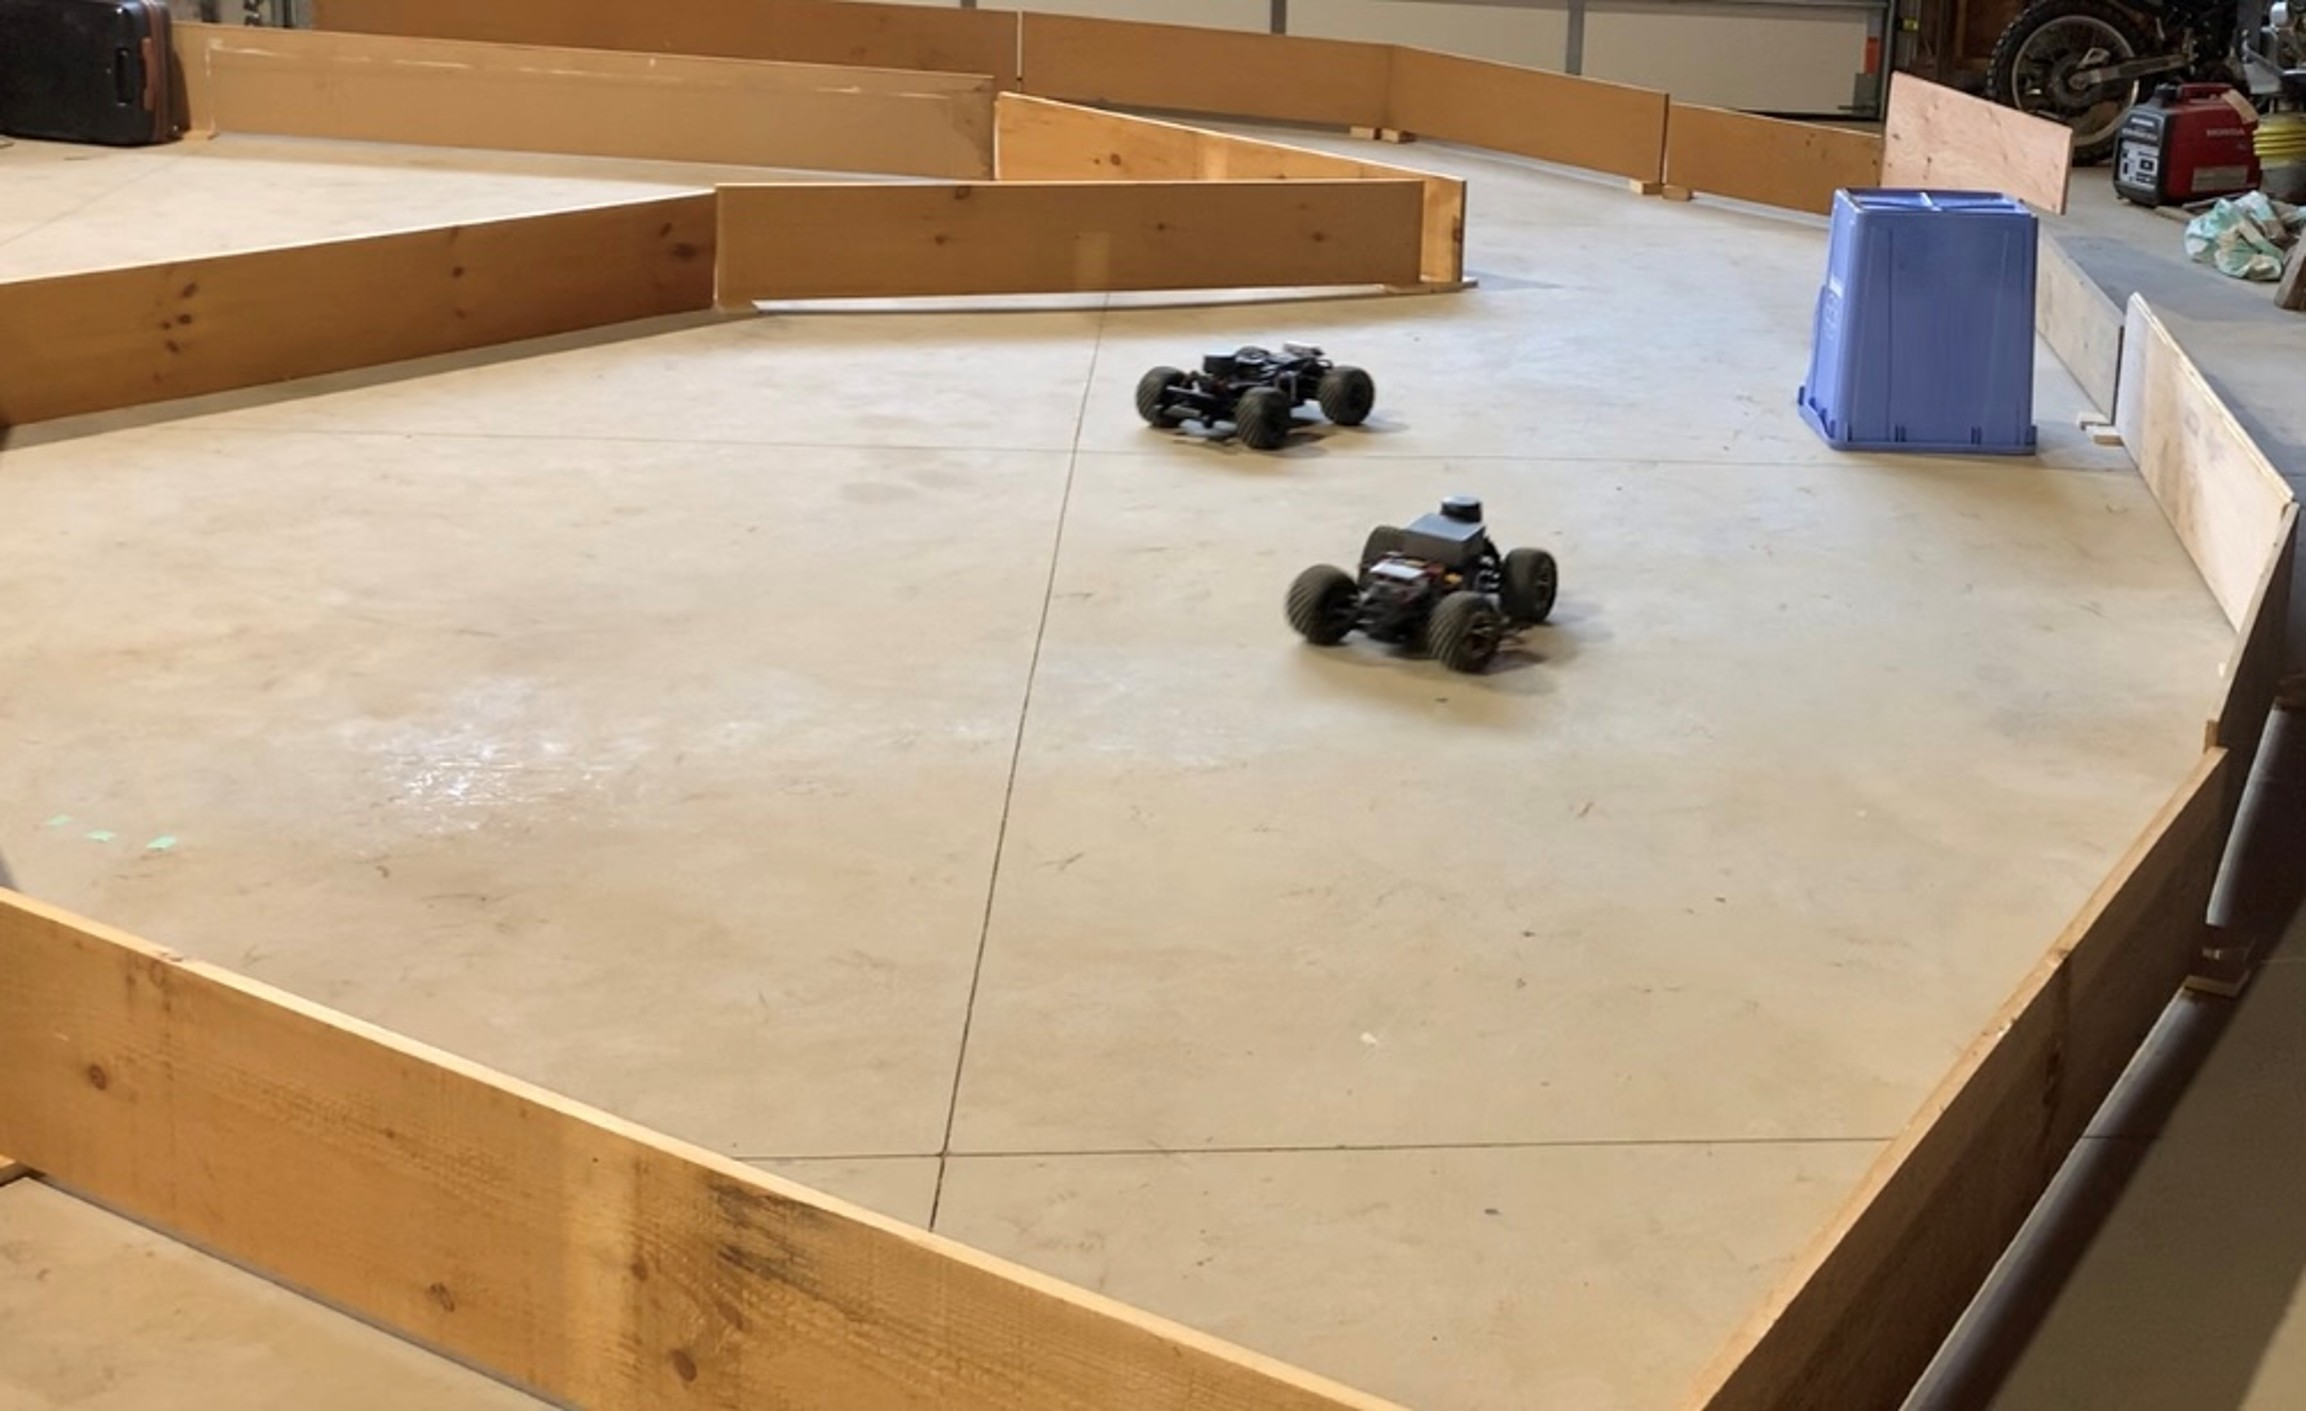
\includegraphics[width=0.95\columnwidth]{Figures/Experiment_Dynamic_Frame.JPG}
% \caption{Standalone local path planning via STLMPC is tested on a 1/10$^{\text{th}}$ scale RC vehicle in an unknown, indoor environment with an adversarial vehicle.}
% \label{ExperimentFrame}
% \end{figure}

In the absence of global knowledge, guarantees of successful global passage are limited, so rather, exploration seeks the safest local path, which can then be integrated in a hierarchical planner for complete global coverage. In this case, standalone local planning faces the dual challenge of generating an optimal trajectory without a global reference and subsequently controlling the vehicle to follow the trajectory. Model Predictive Control (MPC) is a commonly used optimization-based method for tracking reference paths in path planning studies \cite{Yu2021}. However, the problems generated are typically non-convex and non-linear \cite{Weiskircher2017,MPC_Planner}, making it difficult to obtain globally optimal solutions in real time without sacrificing important nonlinearities. In practice, effective locally optimal solutions can be reliably obtained from Sequential Quadratic Programming (SQP)-based solvers \cite{Lim2018,Sabiha22} in real-time if problem-specific insights are leveraged. Local planning is further complicated by the existence of dynamic obstacles, which, if not accurately predicted, can pose high collision risks. Matters are exacerbated when path planning in unknown settings at higher speeds, as conditions can quickly change, risking high-speed collisions. Navigation using safe, dynamic speeds is required for effective racing performance, while assumed knowledge of the course layout or dimensions \cite{Evans24} should be avoided.
\IEEEpubidadjcol
 
%Contributions at the end of this section

Generally, navigation techniques for mobile robots are classified as either global or local planners, where the latter tracks the global path while performing online obstacle avoidance. One such local planner is the Dynamic Window Approach (DWA) \cite{DWA}, which conducts an optimization that prioritizes a heading towards the goal position and clearance of nearby obstacles. Optimization cost weights are fixed, which can lead to poorer performance in different environments, an issue which recent work has sought to address through Reinforcement Learning (RL) \cite{Dobrevski2024}. Additional extensions have introduced dynamic obstacles in the DWA framework \cite{Molinos2019}. Another local planner found in the literature is an elastic band algorithm \cite{EB}, which aims to preserve the nature of the global path while deforming to accommodate obstacle avoidance. The Timed Elastic Band (TEB) planner \cite{TEB} extends on this approach by accounting for constraints on vehicle dynamics. One extension of TEB incorporates a structured strategy for object detection, association and estimation to enable dynamic obstacle avoidance \cite{Dong21}. Parameter tuning can highly impact performance \cite{Yuan2022}, and while MPC extensions of TEB have been explored \cite{Rosmann2015}, MPC has become preferred for local planning of robots with nonholonomic constraints \cite{MPC_Planner}.

One MPC approach uses a 3D potential field method to generate a collision-free reference trajectory that multiconstrained MPC then tracks via motion control, yielding front steering angle commands \cite{Ji2017}. Path following is achieved both using model predictive lateral control \cite{Gao22} and by modelling collision regions as ellipsoids that bound the Minkowski sum of the robot and dynamic obstacle geometries \cite{Brito19}. MPC is also used to reach intermediate goal positions along a global path, while collision avoidance is performed by parameterizing moving obstacles as fixed, blocked regions at time samples \cite{MPC_Planner}.

In other navigation approaches, the role of MPC in path planning increases while also providing motion control. One warehouse application assumes only the goal location is known, using MPC to derive both the optimal local path and control inputs, albeit under significant environmental assumptions \cite{Ishihara2022}. A different study incorporates actuator dynamics and nonholonomic constraints to generate trajectories that terminate at a desired local goal instead of tracking a full reference path \cite{Babu2019}. Efforts have been made to linearize certain problems, where, in some situations, these approximations can decrease computational costs while not significantly degrading performance \cite{Alcal2019}. RL has also been paired with MPC, both in a hierarchical setup \cite{Fehr2025} and using MPC in training. In simple, simulated settings, RL is shown to reduce computation time while generating MPC-comparable paths \cite{Kim2022}.

In the context of autonomous vehicle racing, one approach uses sensor data to extract a local map before estimating the track center line based on curved walls constructed by consecutive obstacles, assuming constant track width \cite{Evans24}. Here and in prior racing studies \cite{Liniger17}, Model Predictive Contouring Control (MPCC) is used to minimize the center line contour following error while concurrently maximizing vehicle speed. MPCC can facilitate real-time implementation through a linear time-varying approach, while ensuring stability via a contraction constraint \cite{Lam2010}. Alternatively, Model Predictive Path Integral (MPPI) control, a sampling-based optimization approach, makes parallel samples in the control space and removes the need for separate planning and execution steps \cite{Williams2016}. By guiding the convergence target of the solution, an extension enhances performance for racing when multimodalities exist in the optimal action distribution \cite{Honda23}. Another study incorporates vehicle overtaking through non-linear MPC in simulation, where overtaking is only enacted if the maneuver has a low risk of collision \cite{Buyval2017}.

To attain universal safe navigation in unknown, dynamic and racing environments, path planning is proposed using the novel Sequential Tracking Line Model Predictive Control (STLMPC) method. The key features and contributions of this approach are detailed as follows.
\begin{enumerate}
\item{Maximization of local obstacle clearance through a real-time generated piecewise linear local reference path.}
\item{Attainment of low-cost and reliable trajectory prediction solutions in real-time using non-convex MPC optimization with smooth, continuous analytical gradients, effective initial guesses and an SQP-based solver. Conformance of trajectory to nonholonomic vehicle constraints and control input limits.}
\item{Temporal incorporation of detected, tracked vehicle trajectories, assuming fixed curvature and velocity, in predictive navigation.}
\item{Navigation at dynamic, high speeds for racing, subject to turning-angle and obstacle-proximity safety conditions.}
\item{Validation of performance in diverse, dynamic environments, both in simulation and experimentally using a 1/10$^{\text{th}}$ scale RC vehicle. Release of open-source implementation in C++/ROS for public use.}
\end{enumerate}
%Then a summary of the remaining sections in this paper

These contributions delineate STLMPC from closely related work. In contrast to the authors' prior non-predictive approach \cite{PD}, which tracks a \emph{single} tracking line via feedback linearization at constant velocity, STLMPC contributes a receding-horizon sequence of tracking lines, a non-convex MPC layer that enforces the nonholonomic model and input-rate limits over the horizon, a dynamic-obstacle prediction branch, and a variable-velocity racing formulation with soft turning- and proximity-based speed limits. Whereas the SVM max-margin construction has been applied to \emph{global}, start-to-goal planning \cite{Miura2006,Morales2016}, here it is solved receding-horizon and sequentially, with no global goal, producing a piecewise-linear local reference rather than a complete path. Section \ref{sec6} quantifies these distinctions through component-wise ablations and against canonical gap-following (FGM) and sampling-based (MPPI) baselines.

The remainder of this paper is organized as follows. Section \ref{sec3} contains the formulation of the novel standalone local path planner, entitled STLMPC, along with extensions that integrate localization and dynamic obstacle avoidance. An adaptation is then formulated in Section \ref{sec5}, which prioritizes safe, high velocities for navigation in racing contexts. Performance validation is conducted in real-world conditions in Section \ref{sec6} before the paper is concluded in Section \ref{sec7}.

\section{Sequential Tracking Line Model Predictive Control}\label{sec3}
This section presents the full framework for STLMPC, starting from the generation of successive tracking lines through to the non-convex MPC optimization. The complete algorithm pseudocode is provided for real-time implementation, and the integration of localization and dynamic obstacle avoidance into standalone local path planning is discussed.
\subsection{Tracking Line Generation}
The local unknown environment is constructed based on a set of $N_{\text{obs}}$ detected obstacles (in practice, through a sensor such as LiDAR) in the moving vehicle base frame. The set is expressed both in Cartesian $\{{(x_{{\text{obs}},i}, y_{{\text{obs}},i})}\}_{i=0}^{N_{{\text{obs}}}-1}$, as well as in polar $\{{(r_{{\text{obs}},i}, \theta_{{\text{obs}},i})}\}_{i=0}^{N_{{\text{obs}}}-1}$ coordinates. The proposed convention assigns $+x$ as the forward vehicle direction, $+y$ as the leftward vehicle direction and $+\theta$ as the counterclockwise rotation direction, beginning from the $+x$ axis. The vehicle state is described by $[x,y,\theta]$ with control inputs $[\delta,v]$, where $x$ and $y$ are the vehicle position coordinates, $\theta$ is the vehicle orientation, $\delta$ is the current steering angle and $v$ is the forward velocity. The fixed wheelbase $l$ describes the distance between the front and rear axles of a given vehicle.

To obtain the reference tracking line, a heading direction is first required. The approach taken, inspired by the Follow the Gap Method (FGM) \cite{Sezer2012}, initially orders the $N_{\text{obs}}$ obstacles in increasing order of $\theta_{\text{obs},i}$ where for all $i \in\{{0,...,N_{\text{obs}}-1}\}$, $-\pi\leq \theta_{\text{obs},i} < \pi$. Using a threshold distance $d_{\text{safe}}$, all obstacles with $r_{\text{obs},i}\leq d_{\text{safe}}$ are assumed to be immediate potential hazards. For all obstacles in the front $\pi$ radian window ($-\frac{\pi}{2}\leq \theta_{\text{obs},i} \leq \frac{\pi}{2}$), the largest range-weighted angular gap with only obstacles further than $d_{\text{safe}}$ is found, providing the gap's start and end angles, $\theta_{\text{start}}$ and $\theta_{\text{end}}$. The safest gap balances the angular size with larger obstacle ranges in the gap and exceeding $d_{\text{safe}}$ to ensure the safest local direction of travel. Once the safest angular gap is found, the heading direction is calculated as $\theta_{\text{head}}=\frac{1}{2}(\theta_{\text{start}}+\theta_{\text{end}})$.

The obstacles are now split into left, right and excluded clusters with respect to the heading angle $\theta_{\text{head}}$ using offsets $a_l,b_l,a_r\ \textup{and}\ b_r$. Obstacles with \mbox{$\theta_{\text{obs},i} \mathbin{\in} [\theta_{\text{head}}\!+\!a_l,\theta_{\text{head}}+b_l]$} belong to the left cluster $\mathcal{O}_l$, while the right cluster $\mathcal{O}_r$ contains obstacles satisfying \mbox{$\theta_{\text{obs},i} \mathbin{\in} [\theta_{\text{head}}-b_r,\theta_{\text{head}}-a_r]$}. The Cartesian forms \mbox{$\mathcal{O}_l=\{{(x_{{\text{obs}},i}, y_{{\text{obs}},i})}\}_{i=0}^{N_{{\text{left}}}-1}$} and \mbox{$\mathcal{O}_r=\{{(x_{{\text{obs}},i}, y_{{\text{obs}},i})}\}_{i=0}^{N_{{\text{right}}}-1}$} are then used in a quadratic optimization to obtain the reference tracking line. Here, $N_{\text{left}}$ and $N_{\text{right}}$ denote the number of left and right obstacles, respectively. In open-space or single-wall cases where a cluster is empty or the admitted gap exceeds a set angular threshold, a synthetic bounding line aligned with $\theta_{\text{head}}$ and offset to the maximum sensor range is substituted for the missing side, so that a well-posed corridor is always defined for \eqref{quadprogopt} and the vehicle continues toward the open direction rather than stalling.

The basis for the tracking line optimization comes from the concept of Support Vector Machines (SVMs) \cite{Cortes1995}, which identify decision boundaries that best separate classes of points by maximizing the margin between them. This approach has been used in global planning to find paths between a start point and goal while maximizing distance to obstacles \cite{Miura2006,Morales2016}. The parallel right and left bounding lines on the obstacle clusters are described respectively (Fig. \ref{cardiagram2}) by $w^Tq+b=1$ and $w^Tq+b=-1$ with $q=[x,y]^T$. Parallel decision boundaries are used here to define a consistent maximum margin and preserve symmetry, forming the basis for the convex optimization problem.

\begin{figure}[ht]
    \centering
    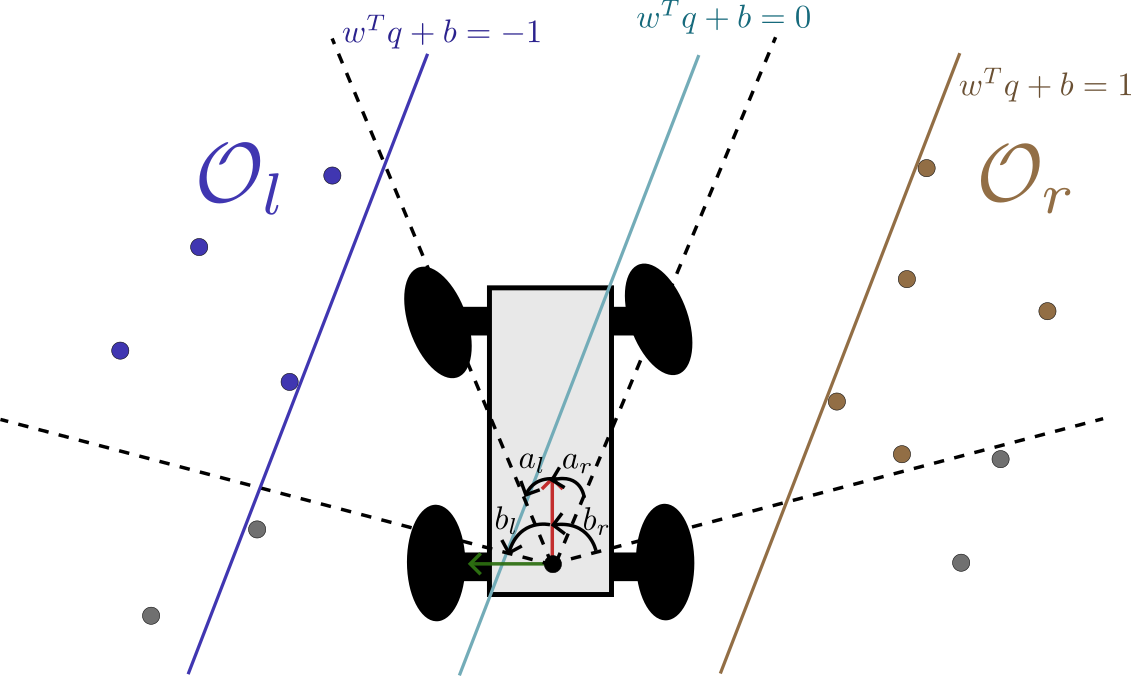
\includegraphics[width=0.95\columnwidth]{Figures/cardiagram2.png}
    \caption{Left and right bounding lines for the defined obstacle clusters, as well as the optimal center tracking line generated.}
    \label{cardiagram2}
\end{figure}

To maximize the distance between the lines $d=\frac{2}{\sqrt{w^Tw}}$, the\vspace{1pt} denominator is minimized via a standard quadratic objective. Linear inequality constraints are developed to ensure obstacles remain on the separated side of each bounding line. Finally, $b$ is bounded to ensure that the (0,0) reference exists between the two bounding lines so that the vehicle is in the middle of the bounded obstacle clusters. The quadratic optimization with linear inequality constraints is proposed by:

\begin{equation}
\begin{aligned}
\min_{w,b} \quad & \frac{1}{2}w^Tw \\
\text{subject to} \quad & w^Tp_i+b-1 \geq 0 \quad \forall p_i \in \mathcal{O}_r\\
                        & w^Tp_j+b+1 \leq 0 \quad \forall p_j \in \mathcal{O}_l\\
                        & -1+\epsilon \leq b \leq 1-\epsilon.\\
\end{aligned}
\label{quadprogopt}
\end{equation}

This problem can be solved through Goldfarb and Idnani's active-set dual method \cite{Goldfarb1983} where $\epsilon$ is small ($\epsilon=0.1$ in implementation) and strict convexity is ensured by including a small quadratic objective term involving $b$. The center line, defined by $w^Tq+b=0$, becomes the reference tracking line, where normalization by $b$ reduces the line parameters from three to two:
\begin{equation}
    w^Tq+1=0, \quad \text{where}\ \ w\leftarrow\frac{1}{b}\,[w_x,w_y]^T.
    \label{normline}
\end{equation}
This is the form used in \eqref{3.1.6} and throughout the ensuing MPC formulation. The bound on $b$ does not exclude the degenerate case $b=0$, where the center line passes through the vehicle reference point; this is handled gracefully since, as $|b|\rightarrow0$, the normalized coefficients grow in magnitude while all ensuing expressions involve only ratios of the form $(w^Tq+1)/\|w\|$, converging to the correct perpendicular distance. For numerical robustness, the implementation clamps $|b|\geq\epsilon_b=10^{-3}$ prior to normalization, displacing the line by at most $\epsilon_b/\|w\|$. Now, in the general case, this process is extended to $n_\text{MPC}$ sequential tracking lines, each with $k_\text{MPC}$ future samples (with sample time $\Delta t$).

Each sequential tracking line is described in the normalized form \eqref{normline} by \mbox{$w_i=[w_{x,i},w_{y,i}]^T$} for \mbox{$i \in \{0,...,n_\text{MPC}-1\}$} where the reference frame \mbox{$p_{\text{base},i}=[x_{\text{base},i},y_{\text{base},i}]^T$} is updated for each tracking line, starting with $p_{\text{base},0}$. From the reference frame point, the closest point on the tracking line $p_{\text{start},i}$ is:
\begin{equation}
\begin{bmatrix}
    x_{\text{start},i}\\
    y_{\text{start},i}
\end{bmatrix}=p_{\text{base},i}-\frac{w_i^Tp_{\text{base},i}+1}{\|w_i\|^2}\cdot w_i.
    \label{3.1.6}
\end{equation}
The tracking line orientation \mbox{$\theta_{\text{track},i}=-\mathrm{atan2}({w_{x,i}},{w_{y,i}})$} and the vehicle's current velocity $v$ are then used to find the end point of the tracking line $p_{\text{end},i}$ through:
\begin{equation}
    \begin{bmatrix}
        x_{\text{end},i}\\
        y_{\text{end},i}
    \end{bmatrix}=p_{\text{start},i}+v\Delta t\,k_\text{MPC}\cdot \begin{bmatrix}
        \cos(\theta_{\text{track},i})\\
        \sin(\theta_{\text{track},i})
    \end{bmatrix}.
    \label{3.1.7}
\end{equation}

This becomes the reference point for the next tracking line, $p_{\text{base},i+1}=p_{\text{end},i}$. All obstacles are transformed from the original reference $p_{\text{base},0}$ (with obstacles denoted $\{{(x^{(0)}_{\text{obs},j}, y^{(0)}_{\text{obs},j})}\}_{j=0}^{N_{\text{obs}}-1}$)  to the new reference $p_{\text{base},i+1}$ (with obstacles denoted $\{{(x^{(i+1)}_{\text{obs},j}, y^{(i+1)}_{\text{obs},j})}\}_{j=0}^{N_{\text{obs}}-1}$) where the process then repeats, starting from finding the best heading direction. After each sequential tracking line is solved for via \eqref{quadprogopt} in its corresponding frame of reference, a normalized transformation is done back to the initial base frame for ensuing \eqref{3.1.6} and \eqref{3.1.7}. The $n_\text{MPC}$ tracking lines described by $w_i$ (Fig. \ref{cardiagram3}) are subsequently used in the MPC optimization as the piecewise linear reference path.

\begin{figure}[ht]
    \centering
    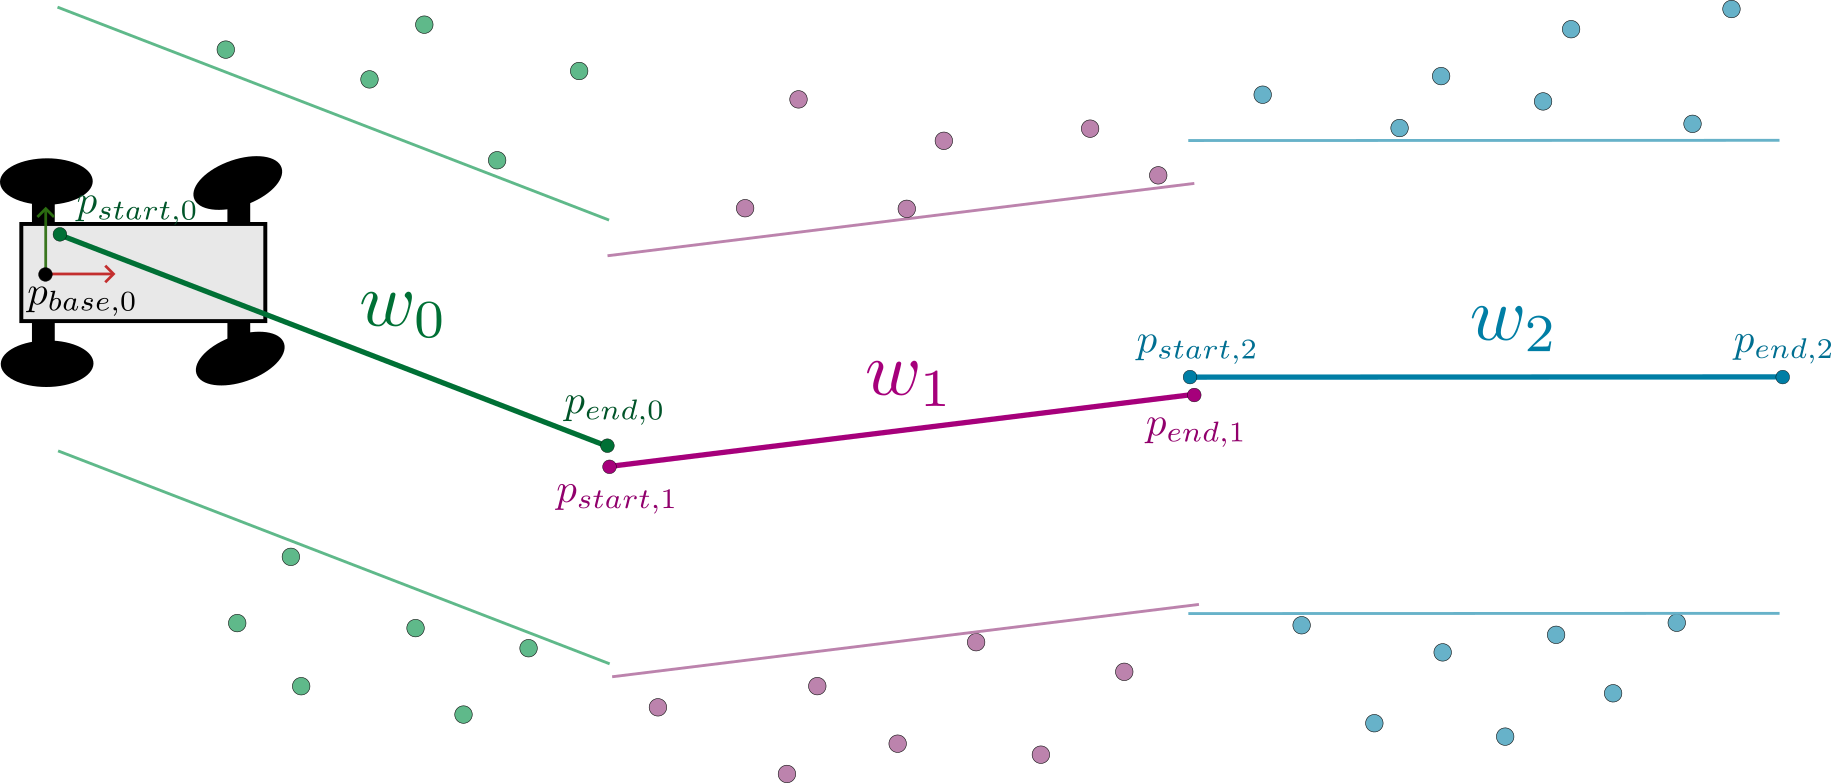
\includegraphics[width=0.95\columnwidth]{Figures/cardiagram3.png}
    \caption[Sequential tracking lines for $n_\text{MPC}=3$]{Sequential tracking lines with bounding lines and respective obstacles for $n_\text{MPC}=3$. Tracking line start and end points are denoted accordingly with respect to the initial base frame.}
    \label{cardiagram3}
\end{figure}

\subsection{MPC Optimization}
In the preliminary formulation of STLMPC, velocity is assumed constant, such that $\delta_i$ represents the control inputs and characterizes the predicted trajectory. The horizon length is $n_\text{MPC}k_\text{MPC}$ samples, while discretization of the state and control input variables [$x,y,\theta,\delta$] produces $4n_\text{MPC}k_\text{MPC}$ optimization variables.

\indent \textit{1) Objective:} The multi-term objective balances tracking of the piecewise linear reference path with expending low control effort over the prediction horizon. Each tracking line is associated with $k_\text{MPC}$ successive samples, obtaining $\tilde w_{i}$ according to $\tilde w_{i}=w_j \ \text{for} \ jk_\text{MPC}\leq i <(j+1)k_\text{MPC},\ j\in\{0,...,n_\text{MPC}-1\}$. A quadratic term is developed to express vehicle proximity to the reference path as a sum of squared Euclidean distances $\!d_i^2$:
\begin{equation}
    F_{d^2}=\sum_{i=0}^{n_\text{MPC}k_\text{MPC}-1} d_i^2 =\sum_{i=0}^{n_\text{MPC}k_\text{MPC}-1}\frac{(\tilde w_i^TP_i+1)^2}{\|\tilde w_i\|^2}
    \label{3.1.13}
\end{equation}
where $P_i=$ $[x_i, y_i]^T$ is the vehicle position at the $i^\text{th}$ sample.

The summation of squared Euclidean distance derivatives $\dot d_i^2$ forms another objective term:
\begin{equation}
    F_{\dot d^2}=\sum_{i=0}^{n_\text{MPC}k_\text{MPC}-2}\dot d_i^2 =\sum_{i=0}^{n_\text{MPC}k_\text{MPC}-2}\frac{(\tilde w_i^T\dot P_i)^2}{\|\tilde w_i\|^2}
    \label{3.1.16}
\end{equation}
which encourages alignment of the vehicle orientation with that of the piecewise linear reference path at every sample. Only $P_i$ is assumed to change over time, disregarding the discontinuous jumps in the otherwise constant $\tilde w_i$ when the next tracking line is followed. Forward differencing is used to obtain $\dot P_i$, making the sum valid for only the first $n_\text{MPC}k_\text{MPC}-1$ samples. The last term captures the cost of control effort as a sum of squared steering angles to reduce unnecessary path oscillations, promoting stability:
\begin{equation}
     F_{\delta^2}=\sum_{i=0}^{n_\text{MPC}k_\text{MPC}-1}\delta_i^2. 
     \label{3.1.17}
\end{equation}

The quadratic construction of the objective is well-suited for standard non-convex solvers, such as the SQP-based SLSQP solver \cite{Kraft1994}, which is implemented. Analytical gradients with respect to each optimization variable are used in the solver for proper numerical accuracy and stability.

\indent \textit{2) Constraints:} To ensure the predicted trajectory satisfies vehicle dynamics and control input limits, equality (denoted by $h$) and inequality (denoted by $g$) constraints are formulated. The initial vehicle position and orientation are fixed to start at the initial base frame, meaning $x_0=0$, $y_0=0$ and $\theta_0=0$. The kinematic bicycle model \cite{Rajamani2012} is used to represent vehicle dynamics, assuming no slip and front-wheel steering, which holds for reasonably low tire slip angles and lateral accelerations \cite{Polack2017}. The resulting non-linear dynamics give rise to non-convex equality constraints, which render the optimization non-convex. These constraints are given for position in $x$:
\begin{align}
    x_{i+1}&=x_i+\Delta t\,v\cos(\theta_i) \quad \forall i\in \{0,...,n_\text{MPC}k_\text{MPC}-2\} \nonumber \\
    h_{x,i} &= x_{i+1} - x_i - \Delta t \, v \cos(\theta_i), \quad h_{x,i} = 0,
    \label{3.1.20}
\end{align}
for position in $y$:
\begin{align}
    y_{i+1}&=y_i+\Delta t\,v\sin(\theta_i) \quad \forall i\in \{0,...,n_\text{MPC}k_\text{MPC}-2\} \nonumber \\
    h_{y,i} &= y_{i+1} - y_i - \Delta t \, v \sin(\theta_i), \quad h_{y,i} = 0,
    \label{3.1.21}
\end{align}
and for orientation in $\theta$:
\begin{align}
    \theta_{i+1}&=\theta_i+\Delta t\frac{v}{l}\tan(\delta_i) \quad \forall i\in \{0,...,n_\text{MPC}k_\text{MPC}-2\} \nonumber \\
    h_{\theta,i} &= \theta_{i+1}-\theta_i-\Delta t\frac{v}{l}\tan(\delta_i), \quad h_{\theta,i} = 0.
    \label{3.1.23}
\end{align}
% These non-convex equality constraints importantly reflect the non-linear vehicle dynamics over the future horizon and cause the optimization to be non-convex.

Control input bounds are incorporated based on the physical limitations of the vehicle, where the maximum steering angle magnitude $\delta_\text{max}$ limits the left (+) and right (-) turning angles:
\begin{equation}
    -\delta_\text{max}\leq\delta_i\leq\delta_\text{max} \quad \forall i\in \{0,...,n_\text{MPC}k_\text{MPC}-1\}.
    \label{steer_con1}
\end{equation}
Additionally, inequality constraints use the maximum steering angle rate of change $\dot\delta_\text{max}$ (in rad/s) to restrict turning angles via forward differencing $\forall i\in \{0,...,n_\text{MPC}k_\text{MPC}-2\}$:
\begin{subequations}
\label{steer_con2}
\begin{align}
    -\Delta t\,\dot\delta_\text{max}&\leq \delta_{i+1}-\delta_i \leq\Delta t\,\dot\delta_\text{max}\nonumber \\
    g_{\delta^+,i}&=\delta_{i+1}-\delta_i -\Delta t\,\dot\delta_\text{max}, &g_{\delta^+,i}\leq0\; \label{3.1.25} \\
    g_{\delta^-,i}&=-\delta_{i+1}+\delta_i -\Delta t\,\dot\delta_\text{max}, &g_{\delta^-,i}\leq0. \label{3.1.26}
\end{align}
\end{subequations}

Finally, the initial steering angle is fixed according to the prior time sample's control input. As the servo motor or steering mechanism used requires time to transition, the control input is applied a sample in advance, which improves stability in practice. Therefore, by the next time sample, the steering angle will be equal to the desired value according to the optimized trajectory. This means $\delta_0=\delta_\text{last}$ where $\delta_\text{last}$ was the steering angle applied as a result of the MPC optimization at the previous control step. The first free predicted steering angle is applied at each control step as $\delta_\text{cmd}=\delta_1$ while analytical gradients are again used for all constraints.

\indent \textit{3) Optimization Problem:} The STLMPC optimization is:
\begin{equation}
\begin{aligned}
\min_{x_j,y_j,\theta_j,\delta_j} \quad & \lambda_{d^2}F_{d^2}+\lambda_{\dot d^2}F_{\dot d^2}+\lambda_{\delta^2}F_{\delta^2} \\
\text{subject to} \quad & g_{\delta^+,i}\leq0,\quad g_{\delta^-,i}\leq0 \\
                        & h_{x,i}=0, \quad h_{y,i}=0,\quad h_{\theta,i}=0\\
                        & -\delta_\text{max}\leq\delta_j\leq\delta_\text{max}\\
                        & x_0=0,\quad y_0=0,\quad \theta_0=0,\quad \delta_0=\delta_\text{last}\\
                        & \forall i\!\mkern-1mu\in\!\! \{\mkern-2mu0,...,\mkern-1.5mun_\textup{MPC}k_\textup{MPC}\mkern-1mu\!-\!\mkern-1mu2\mkern-2mu\},j\!\mkern-1mu\in\!\! \{\mkern-2mu0,...,\mkern-1.5mun_\textup{MPC}k_\textup{MPC}\mkern-1mu\!-\!\mkern-1mu1\mkern-2mu\}
\end{aligned}
\label{STLMPC}
\end{equation}
where each objective term has a base weight, and normalization reduces the number of free parameters from three to two.

\subsection{STLMPC Algorithm Pseudocode}\label{sec3C}
By solving this non-convex problem with non-linear solvers, globally optimal solutions are not guaranteed. To ensure high-quality local optimum solutions are found in the region of the global optimum, effective and feasible initial guesses are required. Algorithm \ref{algo2} outlines the process for obtaining effective, feasible starting guesses that facilitate both convergence and the attainment of low-cost local optimum solutions.

\begin{algorithm}[t]
\caption{Formulation of Starting Guess for STLMPC Optimization}
\label{algo2}
% \SetAlgoLined
\DontPrintSemicolon
\KwIn{Tracking Line Orientations \((\tilde\theta_{\textup{track},i})\),\\
      \hspace{3.25em}Last Steering Angle \((\delta_\textup{last})\)}
\KwOut{\(x_i,y_i,\theta_i,\delta_i\)}

\For{$j = 0$ \KwTo $n_\textup{MPC}-1$}{
    \For{$i = 0$ \KwTo $k_\textup{MPC}-1$}{
        \uIf{\(j=0 \textup{\textbf{ and }}i=0\)}{
            \(\delta_{i+jk_\textup{MPC}}=\delta_\textup{last},\,x_{i+jk_\textup{MPC}}=0\)\;
            \(y_{i+jk_\textup{MPC}}=0,\,\theta_{i+jk_\textup{MPC}}=0\)\;
        }
        \uElse{
        \(\delta_\textup{track}\!=\!\tan^{-1}(\frac{l}{\Delta t\,v}(\tilde\theta_{\textup{track},i+jk_\textup{MPC}}\!-\!\theta_{i+jk_\textup{MPC}}))\)\;\vspace{2pt}
            \uIf{\(\theta_{i+jk_\textup{MPC}}<\tilde\theta_{\textup{track},i+jk_\textup{MPC}}\)}{
                \(\delta_{i+jk_\textup{MPC}}=\min(\delta_{\textup{track}},\delta_{{i+jk_\textup{MPC}}-1}+\Delta t\,\dot\delta_\textup{max},\delta_\textup{max})\)\;
            }\vspace{1pt}
            \uElseIf{\(\theta_{i+jk_\textup{MPC}}>\tilde\theta_{\textup{track},i+jk_\textup{MPC}}\)}{
                \(\delta_{i+jk_\textup{MPC}}=\max(\delta_{\textup{track}},\delta_{{i+jk_\textup{MPC}}-1}-\Delta t\,\dot\delta_\textup{max},-\delta_\textup{max})\)\;
            }
            \(x_{i+jk_\textup{MPC}}=x_{i+jk_\textup{MPC}-1}+\Delta t\,v\cos\theta_{i+jk_\textup{MPC}-1}\)\;
            \(y_{i+jk_\textup{MPC}}=y_{i+jk_\textup{MPC}-1}+\Delta t\,v\sin\theta_{i+jk_\textup{MPC}-1}\)\;   
        }
        \uIf{\(i<k_\textup{MPC}-1\) \textup{\textbf{or}} \(j<n_\textup{MPC}-1\)}{
            \(\theta_{i+jk_\textup{MPC}+1}\!\mkern-1mu=\!\theta_{i+jk_\textup{MPC}}\!+\!\Delta t\frac{v}{l}\tan\delta_{i+jk_\textup{MPC}}\)\;
        }
    }
}

\end{algorithm}

Here, the starting guess aligns the vehicle orientation $\theta_i$ with the orientation $\tilde \theta_{\text{track},i}$ of the sequential tracking lines $\tilde w_i$ in the initial base frame at each sample. All steering angles $\delta_i$ after the fixed $\delta_0$ are found that align the orientations while considering bounds on steering angle magnitude and rate of change. After each future sample, the position and orientation states are updated based on the kinematic bicycle model. The resulting predicted trajectory is \emph{feasible by construction}: since the steering angles are generated subject to the magnitude and rate limits \eqref{steer_con1}--\eqref{steer_con2} and the states are propagated through the exact discrete kinematics \eqref{3.1.20}--\eqref{3.1.23}, the guess satisfies all equality and control-input constraints of \eqref{STLMPC} identically, so the solver is initialized strictly inside the feasible set rather than from an arbitrary point. This structural property---not merely empirical tuning---is what makes the guess an effective warm start, and its quality is quantified by the initial- versus converged-cost statistics reported in Section \ref{sec:simstudies}.

In practice, the tracking line optimizations \eqref{quadprogopt} are solved with the QuadProg++\footnote{\url{https://github.com/liuq/QuadProgpp}} implementation of the Goldfarb--Idnani method, while the MPC problem uses the SLSQP implementation of the NLopt library\footnote{\url{https://nlopt.readthedocs.io/en/latest/NLopt_Algorithms}}, supplied with analytical gradients for the objective and all constraints. The fixed initial states are enforced through coincident lower and upper variable bounds rather than additional equality constraints, reducing the constraint count, while the kinematic equalities and rate-limit inequalities are provided as vectorized constraints with tolerance $10^{-8}$. Two termination conditions ensure the real-time control rate is maintained. First, an $L_1$ norm is used to conclude optimization when the relative change in optimization variables decreases below 0.1\% and further progress is likely to be limited. Additionally, a maximum optimization time of 50 ms is set such that the best solution found up to that point is returned in the case of solver timeout. The complete STLMPC algorithm pseudocode is presented in Algorithm \ref{algo3}: generation of $n_\text{MPC}$ tracking lines, MPC optimization and vehicle actuation using the commands $\delta_\text{cmd}$ and $v_\text{cmd}=v$ at each control step.

\subsection{STLMPC using Localization}

The presented STLMPC algorithm can be extended to incorporate localization to an existing occupancy grid. Local planning remains the intent, as a goal location is not known, and global planning is not conducted. Through localization, however, obstacle coverage is enhanced and the observation range is extended for more accurate future planning decisions. The Adaptive Monte Carlo Localization (AMCL) framework is used, employing a particle filter with adaptive sampling to estimate the robot's moving position in a known map. 

\begin{algorithm}[t]
\caption{STLMPC Algorithm Framework}
\label{algo3}
\DontPrintSemicolon
% \SetAlgoLined

\KwIn{Obstacle Ranges \(\{r^{(0)}_{\textup{obs},i_\textup{obs}}\}\) \& Angles \(\{\theta^{(0)}_{\textup{obs},i_\textup{obs}}\}\), Last Steering Angle ($\delta_\textup{last}$), Constant Speed ($v$)}
\KwOut{Steering Command (\(\delta_\textup{cmd}\)), Constant Speed ($v$)}
$p_{\textup{base},0}=[0,0]^T,\, \theta_{\textup{track},-1}=0$\;
$i_\textup{obs}\in\{0,...,N_\textup{obs}-1\},\, i\in\{0,...,n_\textup{MPC}k_\textup{MPC}-1\}$\;
$\{(x^{(0)}_{\textup{obs},i_\textup{obs}},y^{(0)}_{\textup{obs},i_\textup{obs}})\}\leftarrow\{(r^{(0)}_{\textup{obs},i_\textup{obs}},\theta^{(0)}_{\textup{obs},i_\textup{obs}})\}$\;
\For{$j = 0$ \KwTo $n_\textup{MPC}-1$}{
    $\theta_\textup{head}\leftarrow \textup{SafestAngularGap}(\{(r^{(j)}_{\textup{obs},i_\textup{obs}},\theta^{(j)}_{\textup{obs},i_\textup{obs}})\})$\;\vspace{2pt}
    $\mathcal{O}^{(j)}_l,\mathcal{O}^{(j)}_r\leftarrow \textup{FindObstacleClusters}(\theta_\textup{head},$$\{(x^{(j)}_{\textup{obs},i_\textup{obs}},y^{(j)}_{\textup{obs},i_\textup{obs}})\})$\;\vspace{2pt}
    $w_j\leftarrow\textup{SolveTrackingLineQP}(\mathcal{O}^{(j)}_l,\mathcal{O}^{(j)}_r)$\;\vspace{2pt}
    $w_j\!\mkern-1mu\leftarrow\!\mkern-1mu\textup{TransformtoBaseFrame}(w_j,\mkern-1mup_{\textup{base},j},\mkern-2mu\theta_{\textup{track},j-1})$\;
    $p_{\textup{base},j+1},\theta_{\textup{track},j}\leftarrow \textup{getNextReferenceFrame}(p_{\textup{base},j},w_j,v)$\;\vspace{2pt}
    \mbox{$\{(x^{(j+1)}_{\textup{obs},i_\textup{obs}}\mkern-2mu,\mkern-2muy^{(j+1)}_{\textup{obs},i_\textup{obs}}\mkern-1mu)\}\mkern-5mu\leftarrow\mkern-5mu\textup{NextFrameObs}(p_{\textup{base},j+1},$}\vspace{2pt}
    \hspace{0.6em}$\theta_{\textup{track},j},\{(x^{(0)}_{\textup{obs},i_\textup{obs}},y^{(0)}_{\textup{obs},i_\textup{obs}})\})$\;
}
$\tilde w_i\leftarrow \textup{SampledTrackingLines}(w_j)$\;
$x_i,y_i,\theta_i,\delta_i\leftarrow \textup{MakeStartingGuess}(\tilde w_i,\delta_\textup{last})$\;
$x_i,y_i,\theta_i,\delta_i,\delta_\textup{cmd}\leftarrow \textup{SLSQP\_Opt}(x_i,y_i,\theta_i,\delta_i,v,\tilde w_i)$\;
$\textup{Apply }\delta_\textup{cmd},v_\textup{cmd}=v$ $\textup{, repeat process next control step}$\;

\end{algorithm}


\subsection{STLMPC with Dynamic Obstacle Avoidance}\label{sec4}
The realistic scenario of dynamic obstacles is addressed through a comprehensive multi-stage path planning framework designed for real-time operation in rapidly evolving environments. Detection of other 1/10$^{\text{th}}$-scale RC vehicles is performed using a Convolutional Neural Network (CNN) based on the You Only Look Once (YOLO) framework \cite{Redmon2016}, specifically a custom-trained YOLOv5s model. Multiple object detections are associated with their corresponding tracked vehicles across successive frames, with mechanisms in place to handle both newly appearing and missed detections. Through sensor fusion with an RGB-D camera, a nontrivial transformation from color image pixels to depth pixels enables 3D pose estimation of each detected vehicle. An Extended Kalman Filter (EKF) is then employed to estimate the states of tracked vehicles under a constant velocity and curvature motion model, providing predictions for dynamic obstacle avoidance.

The predicted trajectories are propagated starting from the current time using the kinematic bicycle model, with discretized sample positions denoted by $\{(\hat x_{j,i},\hat y_{j,i})\}$ \mbox{$\forall j\in\{0,...,N_\textup{track}-1\}$}, \mbox{$i\in\{0,...,n_\textup{MPC}k_\textup{MPC}-1\}$}. The future states of the $N_\textup{track}$ tracked vehicles are segmented into successive timeframes to generate the $q^{\text{th}}$ tracking line by:
\begin{align}
    &\mathcal{O}^{(q)}_{\textup{obs}_\textup{tot}} \!\leftarrow\! \mathcal{O}^{(q)}_{\textup{obs}_\textup{tot}} \cup \{(\hat x^{(q)}_{j,i},\hat y^{(q)}_{j,i})\}\nonumber \\ &\text{for}\,\, qk_\textup{MPC}\!\leq\! i\!<\!(q+1)k_\textup{MPC}, \,q \!\in\!\{0,...,n_\textup{MPC}-1\}.
    \label{4.4.2}
\end{align}

Here, $\mathcal{O}^{(q)}_{\textup{obs}_\textup{tot}}=\{(x^{(q)}_{\textup{obs}_\textup{tot}},y^{(q)}_{\textup{obs}_\textup{tot}})\}$ denotes the set of obstacles for the $q^{\text{th}}$ tracking line which is later split into left $\mathcal{O}^{(q)}_{l}$ and right $\mathcal{O}^{(q)}_{r}$ clusters for tracking line generation. Now, the obstacle set for each tracking line is defined as the union of sensor detections \mbox{$\mathcal{O}^{(q)}_\textup{obs}$}, known map obstacles obtained via AMCL \mbox{$\mathcal{O}^{(q)}_{\textup{obs}_\textup{map}}$} (if used), and detected vehicle paths for dynamic obstacle avoidance \mbox{$\mathcal{O}^{(q)}_{\textup{obs}_\textup{det}}$}. To more accurately model the moving vehicle and its shape, the four corners of the vehicle body are extracted based on orientation and position in the future frame, as well as vehicle length $\text{l}_\text{v}$ and width $\text{w}_\text{v}$ dimensions. The discretized outline is then used to generate obstacles for avoidance as opposed to the moving center.

Therefore, for each tracked vehicle at each sampled trajectory point corresponding to the relevant tracking line optimization, the estimated vehicle outline is transformed and interpolated. The interpolated points for each respective tracking line and all other points in $\mathcal{O}^{(q)}_{\textup{obs}_\textup{tot}}$ are used, starting from finding the safest angular gap, through to the quadratic optimization in \eqref{quadprogopt}. With the $n_\textup{MPC}$ tracking lines, STLMPC fulfills the same non-linear optimization as before, but now with tracking lines that perform dynamic obstacle avoidance (Fig. \ref{dynamicSTLMPC}).

\begin{figure}[ht]
    \centering
    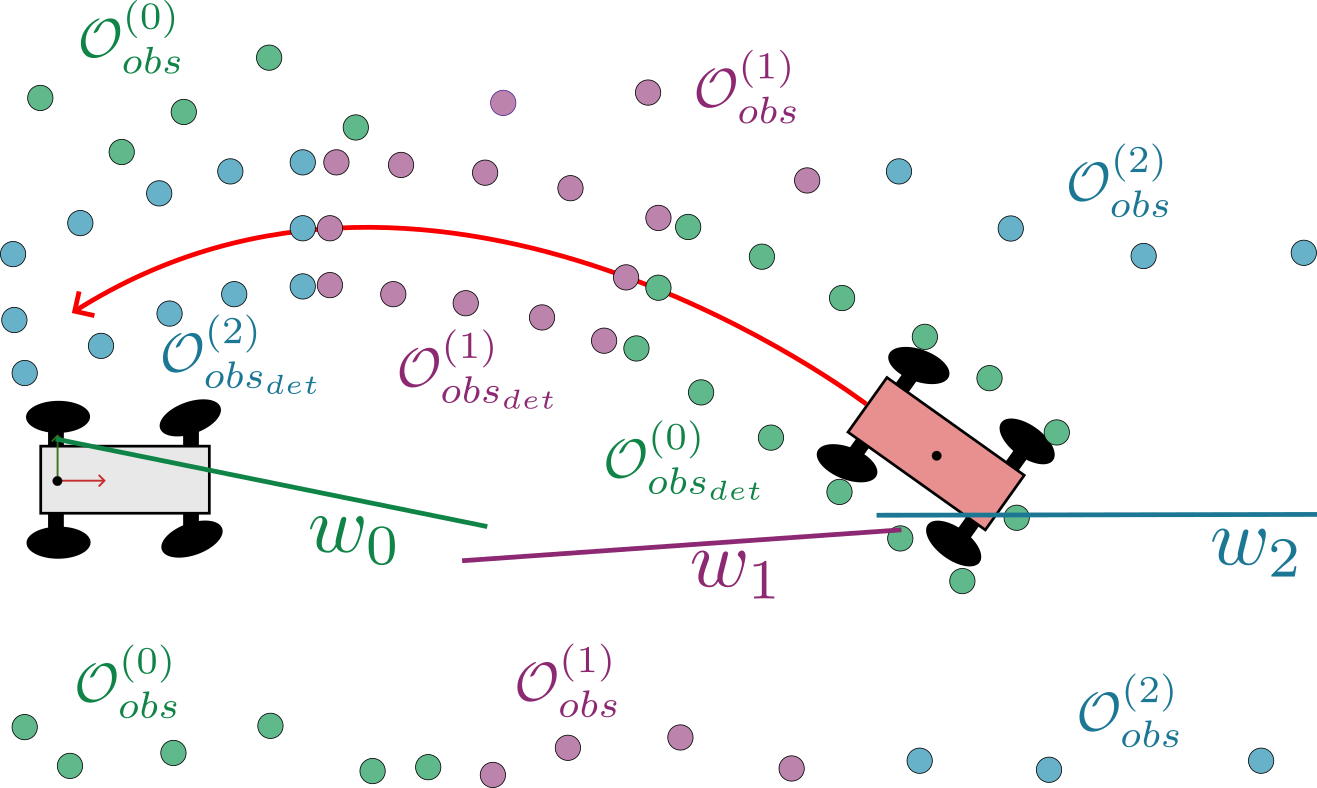
\includegraphics[width=0.9\columnwidth]{Figures/dynamicSTLMPC1.png}
    \caption[Tracking line generation with a dynamic, tracked vehicle]{The detected (red) vehicle's trajectory is predicted and segmented into $n_\textup{MPC}=3$ intervals. The outline of the vehicle along the trajectory is converted into obstacles $\mathcal{O}^{(q)}_{\textup{obs}_\textup{det}}$, which, when added to the static obstacles $\mathcal{O}^{(q)}_\textup{obs}$, generate the three successive reference tracking lines.}
    \label{dynamicSTLMPC}
\end{figure}

\section{Variable-Velocity STLMPC}\label{sec5}
Up to this point, STLMPC assumes a constant velocity over both the predicted trajectory and the course of vehicle operation. This restriction is relaxed in a further extension to handle variable velocities and provide more flexible, higher-dimensional path planning. Higher, safe velocities are prioritized subject to environmental conditions, making racing a natural application of this adapted planning algorithm.

\subsection{Modifications to STLMPC}
%Numbered list as per reference papers for easier reading
Variable-velocity STLMPC follows the same framework as presented in Section \ref{sec3} (with corresponding extensions), except that it now incorporates velocity considerations. The key differences are summarized below.
\begin{enumerate}
\item{The ego vehicle states and control inputs become $[x_i,y_i,\theta_i,\delta_i,v_i]$ $\forall i\in\{0,...,n_\textup{MPC}k_\textup{MPC}-1\}$, thereby denoting a total of $5n_\textup{MPC}k_\textup{MPC}$ optimization variables.}
\item{The objective function has an added velocity-dependent term that prioritizes higher velocities over the horizon.}
\item{Existing constraints now use $v_i$ in place of $v$; the same follows for the ensuing gradients. Control input limits on velocity magnitude and acceleration are implemented.}
\item{A velocity-limiting function is constructed that varies with the steering angle, ensuring that during tighter turns, the vehicle speed is reduced.}
\item{Velocity is limited by proximity to nearby obstacles in the forward direction, ensuring vehicle slowdown to avert head-on collisions.}
\item{The current speed from the electronic speed controller initializes the predicted trajectory as $v_0$, and the first optimized velocity $v_1$ is applied as the commanded speed $v_\textup{cmd}$ alongside the steering angle.}

\end{enumerate}

\subsection{Augmented Optimization Problem}
\indent \textit{1) Augmented Objective:}
For racing applications especially, fast navigation at higher velocities is promoted. This can transfer to more general scenarios where the fastest speed is encouraged, while maintaining safety as defined by subsequent metrics. To encourage quicker trajectories, an additional velocity-dependent term $F_{v^2}$ is introduced into the objective:
\begin{equation}
  F_{v^2}=\sum_{i=0}^{n_\textup{MPC}k_\textup{MPC}-1}\frac{1}{v_i^2}.
  \label{5.2.1}
\end{equation}

This term is similar to the squared sum of steering angles objective term in \eqref{3.1.17}, except now, higher velocities are encouraged, so the reciprocal of each squared velocity is summed and minimized. The new, weighted multi-term objective now becomes $F_{\textup{obj}_v}=\lambda_{d^2}F_{d^2}+\lambda_{\dot d^2}F_{\dot d^2}+\lambda_{\delta^2}F_{\delta^2}+\lambda_{v^2}F_{v^2}$, reusing \eqref{3.1.13}, \eqref{3.1.16} and \eqref{3.1.17}, which depends on both $\delta_i$ and $v_i$ control inputs. Added analytical velocity gradients are incorporated in the optimization solver.

\indent \textit{2) Additional Constraints:}
While pursuing quicker velocity trajectories, the increased flexibility in the optimization means behavior can be further tuned and constrained to meet specific criteria. Control input limits exist for forward velocity magnitude and rate of change, alike those enforced on steering angle in \eqref{steer_con1} and \eqref{steer_con2}. Forward velocity is bounded by maximum $v_\textup{max}$ and minimum $v_\textup{min}$ limits according to:
\begin{equation}
    v_\textup{min}\leq v_i\leq v_\textup{max} \quad \forall i\in \{0,...,n_\textup{MPC}k_\textup{MPC}-1\}
\end{equation}
where $v_\textup{min}$ is set to zero to prevent backwards motion. Linear inequality constraints limit the change in consecutive velocities through the maximum acceleration magnitude $a_\textup{max}$ (in m/$\textup{s}^2$), applied symmetrically to acceleration and braking, \mbox{$\forall i\in \{0,...,n_\textup{MPC}k_\textup{MPC}-2\}$}:
\begin{subequations}
\label{vel_change}
\begin{align}
    -\Delta t\,a_\textup{max}&\leq v_{i+1}-v_i \leq\Delta t\,a_\textup{max}\nonumber \\
    g_{v^+,i}&=v_{i+1}-v_i -\Delta t\,a_\textup{max},& g_{v^+,i}\leq0\; \label{5.3.2} \\
    g_{v^-,i}&=-v_{i+1}+v_i -\Delta t\,a_\textup{max},& g_{v^-,i}\leq0. \label{5.3.3}
\end{align}
\end{subequations}

The velocity control input applied at the prior control step is $v_\textup{last}$, where, as with the steering angle, the DC motor needs time to transition to the next commanded velocity. For this reason, the velocity command $v_\textup{cmd}$ is applied a sample in advance to ensure that by the next control step, it has reached this state per the predicted MPC trajectory. Therefore, the initial velocity in the MPC optimization is fixed by the last command $v_0=v_\textup{last}$ while the first free, predicted velocity is applied as the resulting optimized control input $v_\textup{cmd}=v_1$. In implementation, the initial velocity is additionally floored as $v_0=\max(v_\textup{last},v_\textup{floor})$ with $v_\textup{floor}=0.1$ m/s. Together with a strictly positive, feasible initial guess, the objective term \eqref{5.2.1} then acts as an interior barrier---diverging as any $v_i\rightarrow0^+$---such that optimized velocities remain strictly positive and the nominal bound $v_\textup{min}=0$ is never active, avoiding its singularity even in start-from-rest scenarios.

To preserve vehicle safety at higher speeds, velocity is constrained during turns. If turning with a high instantaneous steering angle $|\delta_i|$, a high instantaneous velocity $v_i$ may cause the vehicle to lose control, skid, or, in the worst case, rollover. Thus, a velocity-limiting function $f_{v_\textup{steer}}$ with smooth gradients is used to set the maximum allowable velocity depending on the current steering angle magnitude. The limit decreases from $v_\textup{max}$ when the turning angle is zero to $\frac{v_\textup{max}}{2}$ when the steering angle magnitude equals $|\delta_\textup{max}|$. Inequality constraints ensure that the velocity at each sample satisfies this limit:
\begin{subequations}
\begin{align}
    f_{v_{\textup{steer},i}}&=\frac{v_\textup{max}}{1+(\frac{\delta_i}{\delta_\textup{max}})^2}\\
    v_i&\leq f_{v_{\textup{steer},i}} \quad \forall i\in\{0,...,n_\textup{MPC}k_\textup{MPC}-1\}  \nonumber \\
    g_{v_\textup{steer},i}&=v_i-\frac{v_\textup{max}}{1+(\frac{\delta_i}{\delta_\textup{max}})^2},\quad g_{v_\textup{steer},i}\leq0.
    \label{5.3.5}
\end{align}
\end{subequations}

To handle tight spaces with collision risks in close proximity to the vehicle, velocity is reduced. Hazards in front of the agent present immediate dangers where the vehicle must either swerve around or brake. A safe stopping distance is identified to slow the vehicle down and prevent head-on collisions while considering the vehicle's maximum deceleration. This ensures the vehicle navigates safely in crowded spaces while braking to a stop in the worst case, if no safe path exists.

Using the total obstacle set in the vehicle base frame, computational tractability is maintained by using the subsampled set $\mathcal{O}_{\textup{obs}_\textup{sub}}=\{{(x_{\textup{obs}_\textup{sub},j}, y_{\textup{obs}_\textup{sub},j})}\}_{j=0}^{N_{\textup{obs}_\textup{sub}}-1}$ where all $N_{\textup{obs}_\textup{sub}}$ subsampled obstacles are spaced by at least $d_\textup{sep}$. The distance between the predicted vehicle position at sample $i$ and the $j^{\text{th}}$ obstacle is \mbox{$d_{i,j}=\sqrt{(x_i-x_{\textup{obs}_\textup{sub},j})^2+(y_i-y_{\textup{obs}_\textup{sub},j})^2}$} while the heading angle in the base frame from predicted vehicle to obstacle is $\theta_{i,j}=\mathrm{atan2}({y_{\textup{obs}_\textup{sub},j}-y_i},{x_{\textup{obs}_\textup{sub},j}-x_i})$.\vspace{2pt}

However, the predicted vehicle's orientation in the base frame is $\theta_i$. Thus, the obstacle heading with respect to this orientation, $\theta_{\text{diff},i,j}=\mathrm{atan2}({\sin(\theta_{i,j}-\theta_i)},{\cos(\theta_{i,j}-\theta_i)})$, is used, where the angular difference is wrapped to the normalized range $(-\pi,\pi]$. To consider only hazardous obstacles ahead of the vehicle during each future sample (Fig. \ref{vehicle_slowdown}), a passband is constructed by $-\theta_{\text{band}_{\textup{max}}} \leq \theta_{\text{diff},i,j}\leq \theta_{\text{band}_{\textup{max}}}$ where $\theta_{\text{band}_{\textup{max}}}$ is the maximum angular difference at which an obstacle is considered. The minimum vehicle-to-obstacle distance in the passband $d_{\text{band}_{\textup{min}}}$ is used in a velocity-limiting function to slow the vehicle when objects are close ahead.

\begin{figure}[ht]
    \centering
    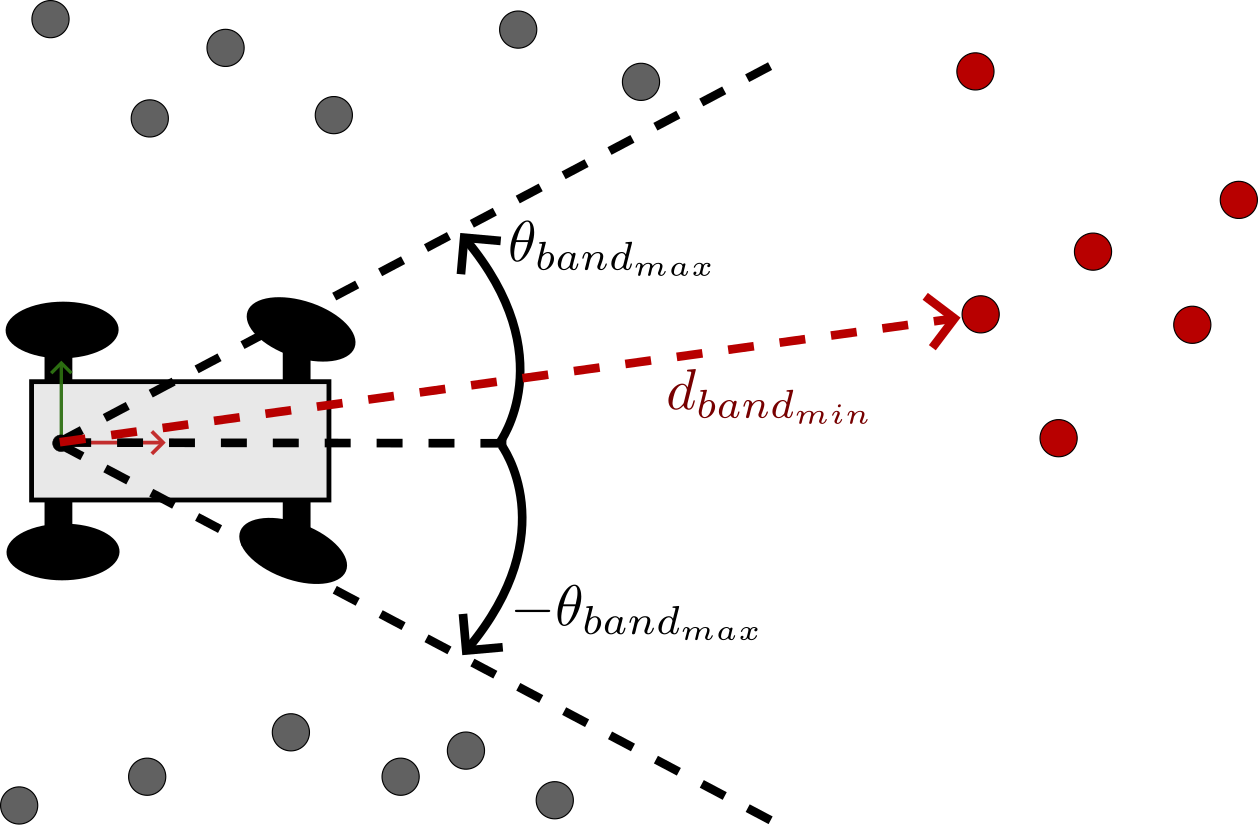
\includegraphics[width=0.7\columnwidth]{Figures/vehicle_slowdown.png}
    \caption[Minimum forward obstacle proximity for vehicle slowdown]{Passband obstacles (red) and minimum obstacle proximity $d_{\text{band}_{\textup{min}}}$.}
	\label{vehicle_slowdown}
\end{figure}

The smooth bandpass function $\theta_{\text{band},i,j}$ uses transition steepness $s_{\theta}$ to only consider obstacles in the vehicle's front field of view and ensure continuous, derivable analytical gradients:
\begin{equation}
    \theta_{\text{band},i,j}=\frac{1}{1+e^{-s_{\theta}(\theta_{\text{diff},i,j}+\theta_{\text{band}_{\textup{max}}})}}-\frac{1}{1+e^{-s_{\theta}(\theta_{\text{diff},i,j}-\theta_{\text{band}_{\textup{max}}})}}.
\end{equation}
In practice, $\theta_{\text{band}_{\textup{max}}}$ is selected such that the passband spans approximately the vehicle's swept width, with margin, at braking-relevant ranges, while $s_{\theta}$ is set sufficiently large that the band edges are sharp relative to the LiDAR angular resolution yet remain smooth for the gradient-based solver. Next, a weighted softmin function produces the minimum forward obstacle proximity $d_{\text{band}_\textup{min},i}$ at sample $i$ through:
\begin{equation}
    d_{\text{band}_\textup{min},i}=-\frac{1}{\beta_v}\log(\sum_{j=0}^{N_{\textup{obs}_\textup{sub}}-1}\theta_{\text{band},i,j}\,e^{-{\beta_v}d_{i,j}}).
    \label{5.3.11}
\end{equation}
Note that $d_{\text{band}_\textup{min},i}$ is not a geometric quantity formed by directly merging angle and range; rather, it is an angularly-weighted soft minimum of the obstacle distances, in which $\theta_{\text{band},i,j}$ acts purely as a front-field relevance weight. Obstacles within the passband ($\theta_{\text{band},i,j}\approx1$) contribute their true distances $d_{i,j}$, whereas obstacles outside it are effectively assigned inflated distances \mbox{$d_{i,j}-\ln(\theta_{\text{band},i,j})/\beta_v\rightarrow\infty$} and are thereby ignored. Fig. \ref{fig:softmin} illustrates the combined coefficient $\theta_{\text{band},i,j}\,e^{-\beta_v d_{i,j}}$ and the corresponding effective distance over obstacle angle and range for the experimental parameter values, where within the passband, the effective distance reduces to the true distance. The approximation sharpness is controlled by $\beta_v$, where higher values more accurately model the true minimum but with poorer numerical stability. Using the softmin function as a smooth approximation ensures continuous gradients and numerical stability for the optimization solver.

\begin{figure}[ht]
    \centering
    \subfloat[]{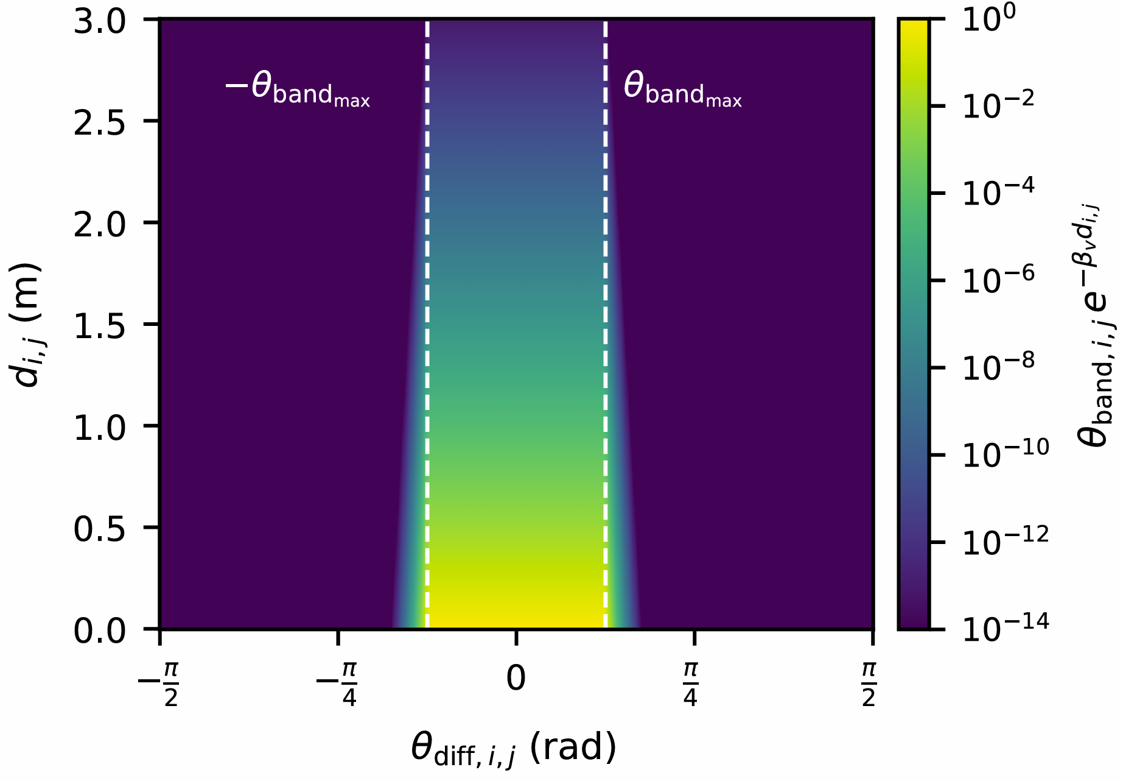
\includegraphics[width=0.24\textwidth]{Figures/fig_softmin_coefficienta.png}}\label{fig_softmin_coefficienta} \hfil
  \subfloat[]{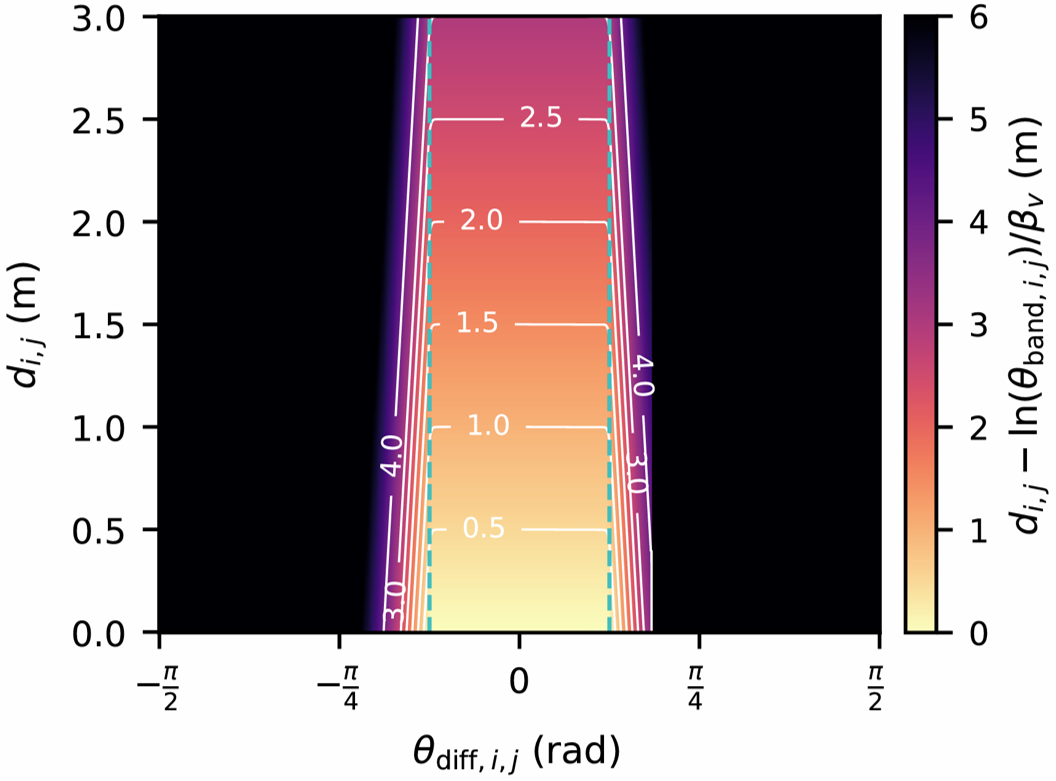
\includegraphics[width=0.24\textwidth]{Figures/fig_softmin_coefficientb.png}}\label{fig_softmin_coefficientb}
    \caption[Softmin weighting coefficient and effective distance]{(a) The combined softmin coefficient $\theta_{\text{band},i,j}\,e^{-\beta_v d_{i,j}}$ over obstacle heading difference and distance for $\theta_{\text{band}_{\textup{max}}}\!=\!\frac{\pi}{8}$ rad, $s_{\theta}\!=\!200\ \textup{rad}^{-1}$ and $\beta_v\!=\!10\ \textup{m}^{-1}$. (b) The corresponding effective distance contribution $d_{i,j}-\ln(\theta_{\text{band},i,j})/\beta_v$, which reduces to the true distance within the passband and diverges outside it.}
    \label{fig:softmin}
\end{figure}

The velocity-limiting function based on forward obstacle proximity $f_{v_{\textup{obs},i}}$ is represented by an exponential term, dependent on $d_{\text{band}_\textup{min},i}$. Here, $d_\textup{stop}$ denotes the obstacle distance at which the vehicle is forced to stop, and the decay rate $\alpha_v$ controls how sharp the velocity limit decrease is as $d_{\text{band}_\textup{min},i}$ is reduced. The inequality constraints ensure the velocity limit is respected at each sample over the prediction horizon:

\begin{subequations}
    \begin{align}
    f_{v_{\textup{obs},i}}&=v_\textup{max}(1-e^{-\frac{d_{\text{band}_\textup{min},i}-d_\textup{stop}}{\alpha_v}})\\
    v_i&\leq f_{v_{\textup{obs},i}} \quad \forall i\in\{0,...,n_\textup{MPC}k_\textup{MPC}-1\}  \nonumber \\
    g_{v_\textup{obs},i}&=v_i-v_\textup{max}(1-e^{-\frac{d_{\text{band}_\textup{min},i}-d_\textup{stop}}{\alpha_v}}),\quad g_{v_\textup{obs},i}\leq0.
    \label{5.3.13}
\end{align}
\end{subequations}

For $d_{\text{band}_\textup{min},i}<d_\textup{stop}$, the limit $f_{v_{\textup{obs},i}}$ becomes negative and, with $v_\textup{min}=0$, would render the constraint set infeasible. This regime is therefore governed by a supervisory stop condition outside the optimization: when the current minimum forward obstacle distance falls below $d_\textup{stop}$, $v_\textup{cmd}=0$ is commanded directly, braking the vehicle to rest. Once the path ahead clears, $v_0=v_\textup{floor}$ re-seeds the optimization and the vehicle accelerates away subject to \eqref{vel_change}, ensuring well-posed behavior in near-stop scenarios.

\indent \textit{3) Extended Optimization Formulation:}
The new problem modifies \eqref{STLMPC}, the original STLMPC optimization, to yield:
\vspace{-2pt}
\begin{equation}
\begin{aligned}
\min_{x_j,y_j,\theta_j,\delta_j,v_j} \quad\!\!\! & \lambda_{d^2}F_{d^2}+\lambda_{\dot d^2}F_{\dot d^2}+\lambda_{\delta^2}F_{\delta^2}+\lambda_{v^2}F_{v^2} \\
\text{subject to} \quad\!\!\! & g_{\delta^+,i}\leq0,\mkern-5mu\quad g_{\delta^-,i}\leq0,\mkern-5mu\quad g_{v^+,i}\leq0,\mkern-5mu\quad g_{v^-,i}\leq0\\                                    &g_{v_\textup{steer},j}\leq0,\quad g_{v_\textup{obs},j}\leq0 \\
                        & h_{x,i}=0, \quad h_{y,i}=0,\quad h_{\theta,i}=0\\
                        & -\delta_\textup{max}\leq\delta_j\leq\delta_\textup{max},\quad v_\textup{min}\leq v_j\leq v_\textup{max}\\
                        & x_0=0,\ y_0=0,\ \theta_0=0,\ \delta_0=\delta_\textup{last},\ v_0=v_\textup{last}\\
                        & \forall i\!\mkern-1mu\in\!\! \{\mkern-2mu0,...,\mkern-1.5mun_\textup{MPC}k_\textup{MPC}\mkern-1mu\!-\!\mkern-1mu2\mkern-2mu\},j\!\mkern-1mu\in\!\! \{\mkern-2mu0,...,\mkern-1.5mun_\textup{MPC}k_\textup{MPC}\mkern-1mu\!-\!\mkern-1mu1\mkern-2mu\}
\end{aligned}
\label{NonUniformV-STLMPC}
\end{equation}
where all existing instances of $v$ in STLMPC now use $v_j$. The initial optimization guess follows the framework detailed in Algorithm \ref{algo2} where $v_j$ replaces $v$ and each velocity variable is initialized to a constant for simplicity, such as $v_\textup{last}$ or $\frac{v_\textup{max}}{2}$.

With higher velocities promoted if safe, the solver provides solutions with varying velocity over the predicted trajectory's time horizon. SLSQP is retained as the optimization solver and the optimized trajectory is provided by $[x_j,y_j,\theta_j,\delta_j,v_j],$ \mbox{$j\in\{0,...,n_\textup{MPC}k_\textup{MPC}-1\}$}. The first free steering angle and velocity variables $\delta_1\,\&\,v_1$ are applied as $\delta_\textup{cmd}\,\&\,v_\textup{cmd}$, and the process repeats at the next control step (as in Algorithm \ref{algo3}).


\section{Performance Evaluation}\label{sec6} %Simulation studies first (breadth), then real-world validation
The performance of the STLMPC planner is now evaluated in static, dynamic and racing environments. The system architecture, testing environment, and local planners used for comparison are first described. Controlled simulation studies (Section \ref{sec:simstudies}) then isolate the contribution of individual components, assess parameter sensitivity, and probe robustness under conditions difficult to reproduce on hardware, with each configuration repeated over 10 randomized trials to provide breadth and statistical repetition. Real-world experiments finally validate that this behaviour transfers to a physical vehicle, reporting Section \ref{sec3}'s STLMPC and the extensions in Section \ref{sec4} and Section \ref{sec5} across static (Experiment \#1), dynamic (Experiment \#2) and racing (Experiment \#3) settings. For each experiment, the performance of the novel local planner is recorded on video.

\subsection{Experimental Setup} %Include the block diagram
For testing and implementation of the planning approaches outlined in this paper, both simulation and experimental environments are used. Simulation testing uses the \textit{f1tenth\_simulator} environment \cite{Babu2020} across varying unknown maps with simulated laser scan data and vehicle detection. The open-source navigation software stack designed using STLMPC is implemented primarily in C++ using ROS Noetic.

Two complementary evaluation settings are used. The hardware experiments of Sections~\ref{sec:exp1}--\ref{sec:exp3} are conducted on three physical courses of increasing difficulty---static, dynamic and racing. The simulation studies are run separately in the \textit{f1tenth\_simulator} on its own set of five unknown maps (Maps~\#1--\#5), distinct from the physical courses, providing the map diversity and repeated trials that are impractical to reproduce physically. Importantly, the scenario type is determined by the planner configuration rather than the map: static and racing studies run the constant- and variable-velocity STLMPC variants of Sections~\ref{sec3} and~\ref{sec5}, while dynamic scenarios additionally inject a scripted adversary that is tracked by the Section~\ref{sec4} branch. Accordingly, the component ablations and sensitivity analysis are conducted on maps with sustained corners (chiefly Map~\#4, a tight switchback), where corner clipping and turn-dependent speed reduction are most pronounced; the dynamic scenarios use an open map (Map~\#2); and generalization is assessed on two further maps not used in the ablations, including a forked layout (Maps~\#3 and~\#5).

Experimental testing is conducted using a 1/10$^{\text{th}}$ scale RC vehicle platform. Relevant hardware includes the NVIDIA Jetson AGX Orin, RPLIDAR A2M8 laser scanner, BNO055 IMU and RealSense D435i RGB-D camera. The system architecture is described in Fig. \ref{block_diagram}, where sensor data is used for static and dynamic obstacle detection before planning. The electronic speed controller, VESC, provides vehicle actuation through control input commands. The laser scanner, \mbox{RGB-D} camera, and IMU module publish data at about 10, 30 and 100 Hz, respectively, resulting in an overall control rate of 10 Hz.

\begin{figure}[ht]
    \centering
    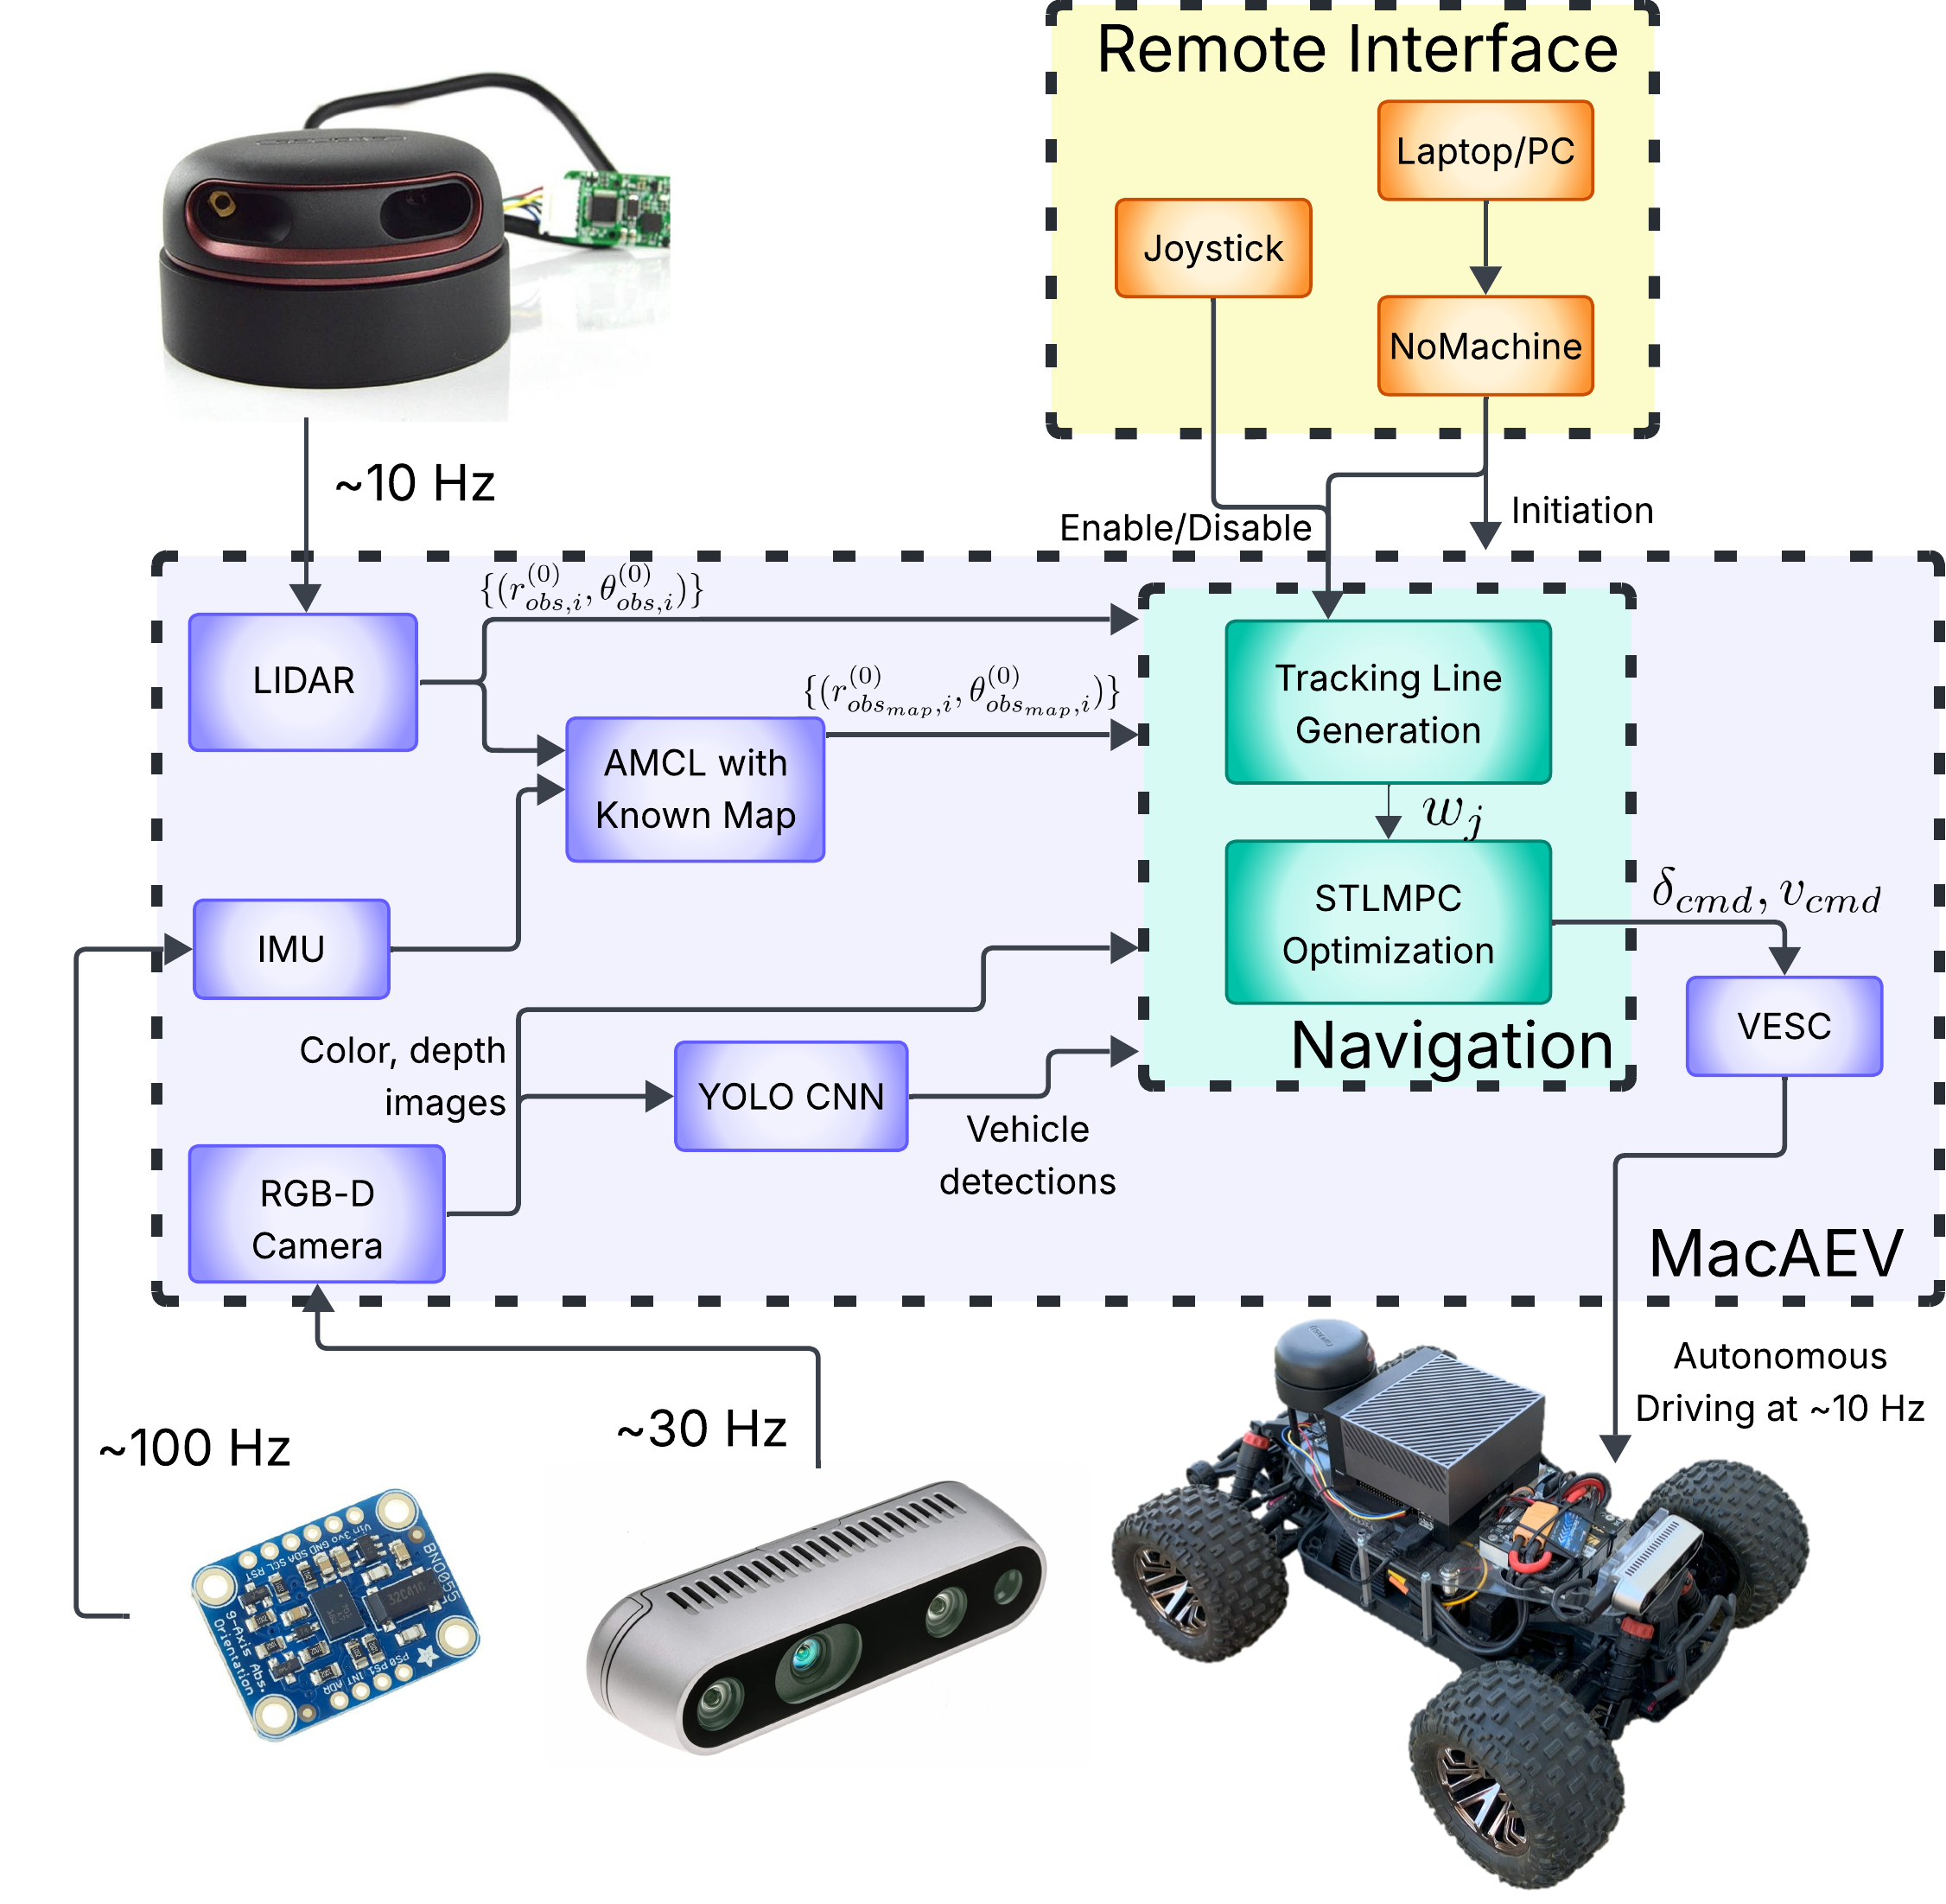
\includegraphics[width=1\columnwidth]{Figures/block_diagram_less_notation.png}
    \caption[System architecture block diagram]{The integrated system's block diagram, which illustrates the sensors used, navigation framework, actuation and remote interfacing with the target machine. In simulation, sensors and vehicle actuation are replicated.}
	\label{block_diagram}
\end{figure}

In testing, STLMPC is evaluated against other local path planning methods, and performance is contrasted. These methods follow the standard ROS navigation stack where the central \textit{move\_base} node links a local and global planner, integrated via \textit{nav\_core}, to achieve navigation and obstacle avoidance using 2D occupancy grid costmaps. As this paper explores navigation in unknown environments, no global goal location is provided, and instead, these planners use a common exploration package, \textit{explore\_lite}. This method updates unexplored frontiers in real-time, where in these tests, the largest one ahead of the vehicle is used as the current goal. 

The global planner then plots a path to the time-varying goal while the local planner performs collision avoidance, yielding the optimized path for immediate motion. Three common ROS local planners---\textit{dwa\_local\_planner} \cite{DWA}, \textit{teb\_local\_planner} \cite{TEB} and \textit{mpc\_local\_planner} \cite{MPC_Planner}---are used with default parameters, except for those relating to the kinematics and properties of the specific vehicle used. Additionally, a non-predictive PD (Proportional-Derivative) approach \cite{PD} is compared. This scheme generates a single tracking line (through the QP approach used in STLMPC) at each control step and maintains tracking by performing feedback linearization to obtain each step's steering angle control input, assuming constant velocity. A Follow-the-Gap Method (FGM) baseline \cite{Sezer2012} is also included in the simulation studies: the gap heuristic that inspired STLMPC's heading is applied in its canonical form, using the geometric gap-centre angle (the median vector to the midpoint of the two gap-bounding obstacles) and steering toward it by feedback linearization at constant velocity. As STLMPC targets goal-free navigation, the FGM goal-fusion term is omitted, so the heading reduces to the gap-centre angle. In contrast to the PD scheme, FGM constructs no tracking line and steers directly on the gap-centre heading, omitting both the QP and the MPC layers; the two baselines therefore bracket STLMPC's contributions---FGM isolating the value of the QP and MPC layers together, and PD isolating the MPC layer given a single QP line. A sampling-based Model Predictive Path Integral (MPPI) planner \cite{Williams2016} is additionally compared as a solver-only substitution: it optimizes the identical STLMPC objective and constraints (Section \ref{sec:simstudies}) by weighted sampling of kinematically-feasible rollouts rather than SQP, isolating the effect of the optimizer itself. For reproducibility, the complete set of STLMPC parameter values used across all experiments is consolidated in Table \ref{tab:params}, with solver settings as detailed in Section \ref{sec3C}.

\begin{table}[ht]
\caption{STLMPC parameter values used in the experiments}
\label{tab:params}
\vspace{-8pt}
\centering
\begin{tabular}{l@{\hskip 5pt}l@{\hskip 6pt}c@{\hskip 8pt}c}
\toprule\\[-0.85em]
\scriptsize Symbol & \scriptsize Description & \scriptsize Exp. \#1/\#2 & \scriptsize Exp. \#3\\
\midrule\\[-0.85em]
\scriptsize $l$ & \scriptsize Wheelbase (m) & \scriptsize 0.287 & \scriptsize 0.287 \\
\scriptsize $\Delta t$ & \scriptsize Sample time (s) & \scriptsize 0.1 & \scriptsize 0.1 \\
\scriptsize $n_\textup{MPC}$, $k_\textup{MPC}$ & \scriptsize Tracking lines, samples per line & \scriptsize 2, 8 & \scriptsize 2, 8 \\
\scriptsize $\delta_\textup{max}$ & \scriptsize Max. steering angle (rad) & \scriptsize 0.4189 & \scriptsize 0.4189 \\
\scriptsize $\dot\delta_\textup{max}$ & \scriptsize Max. steering rate (rad/s) & \scriptsize 3.2 & \scriptsize 3.2 \\
\scriptsize $v$ & \scriptsize Constant velocity (m/s) & \scriptsize 1.5 & \scriptsize --- \\
\scriptsize $v_\textup{min}$, $v_\textup{max}$ & \scriptsize Velocity bounds (m/s) & \scriptsize --- & \scriptsize 0, 3 \\
\scriptsize $a_\textup{max}$ & \scriptsize Max. acceleration (m/$\textup{s}^2$) & \scriptsize --- & \scriptsize 2.5 \\
\scriptsize $v_\textup{floor}$ & \scriptsize Initial velocity floor (m/s) & \scriptsize --- & \scriptsize 0.1 \\
\scriptsize $d_\textup{safe}^{\,\dagger}$ & \scriptsize Gap hazard threshold (m) & \scriptsize 2 & \scriptsize 1.25 \\
\scriptsize $a_l\!=\!a_r$, $b_l\!=\!b_r$ & \scriptsize Cluster offsets (rad) & \scriptsize $\frac{\pi}{9}$, $\frac{\pi}{2}$ & \scriptsize $\frac{\pi}{9}$, $\frac{\pi}{2}$ \\[0.2em]
\scriptsize $\epsilon$, $\epsilon_b$ & \scriptsize QP bound margin, norm. clamp & \scriptsize 0.1, $10^{-3}$ & \scriptsize 0.1, $10^{-3}$ \\
\scriptsize $\lambda_{d^2}$, $\lambda_{\dot d^2}$, $\lambda_{\delta^2}$ & \scriptsize Objective base weights & \scriptsize 1, 30, 1 & \scriptsize 1, 30, 1 \\
\scriptsize $\lambda_{v^2}$ & \scriptsize Velocity objective weight & \scriptsize --- & \scriptsize 1 \\
\scriptsize $\theta_{\text{band}_{\textup{max}}}$ & \scriptsize Passband half-width (rad) & \scriptsize --- & \scriptsize $\frac{\pi}{8}$ \\[0.2em]
\scriptsize $s_{\theta}$ & \scriptsize Passband steepness ($\textup{rad}^{-1}$) & \scriptsize --- & \scriptsize 200 \\
\scriptsize $\beta_v$ & \scriptsize Softmin sharpness ($\textup{m}^{-1}$) & \scriptsize --- & \scriptsize 10 \\
\scriptsize $d_\textup{stop}^{\,\dagger}$ & \scriptsize Supervisory stopping distance (m) & \scriptsize --- & \scriptsize 0.5 \\
\scriptsize $\alpha_v$ & \scriptsize Velocity limit decay rate (m) & \scriptsize --- & \scriptsize 0.5 \\
\scriptsize $d_\textup{sep}$ & \scriptsize Obstacle subsampling spacing (m) & \scriptsize --- & \scriptsize 0.2 \\
\scriptsize $\text{l}_\text{v}$, $\text{w}_\text{v}$ & \scriptsize Detected vehicle length, width (m) & \scriptsize 0.5, 0.4 & \scriptsize --- \\
\bottomrule\\[-0.85em]
\multicolumn{4}{@{}p{0.97\columnwidth}@{}}{\scriptsize $^\dagger$ The values listed are those of the physical courses. The simulation studies of Section \ref{sec:simstudies} run on the larger simulator maps and use the correspondingly larger $d_\textup{safe}=2$~m and $d_\textup{stop}=0.8$~m; all other values are unchanged.}
\end{tabular}
\end{table}

\subsection{Simulation Studies}\label{sec:simstudies}
The planner is first characterized comprehensively in the \textit{f1tenth\_simulator}, where the breadth and statistical repetition impractical on hardware isolate the contribution of individual components, assess parameter sensitivity, and probe robustness; the real-world experiments of Sections \ref{sec:exp1}--\ref{sec:exp3} then validate that this behaviour transfers to a physical vehicle. Studies are run on the simulator maps introduced in Section~\ref{sec6}, with the scenario type set by the planner and adversary configuration rather than the map. Each configuration is repeated over $n=10$ trials with randomized start pose ($\pm0.3$~m in position, $\pm10^{\circ}$ in heading); all simulation results are reported as mean~$\pm$~standard deviation together with the success rate (fraction of trials completing without collision). Throughout Section \ref{sec6}, planner performance is measured by the minimum and average obstacle proximity over a run ($\min_{\tilde k} d_{\textup{min},\tilde k}$, $\bar d_\textup{min}$, where $\tilde k$ indexes the control step and $d_{\textup{min},\tilde k}$ is the closest obstacle to the vehicle at $\tilde k$), the control-input averages and variances ($\overline{|\delta_{\textup{cmd},\tilde k}|}$, $\mathrm{Var}(\delta_{\textup{cmd},\tilde k})$, $\bar v_{\textup{cmd},\tilde k}$, $\mathrm{Var}(v_{\textup{cmd},\tilde k})$), and the course time $t_\textup{tot}$; the simulation studies additionally report the success rate and, for dynamic scenarios, the minimum Time-to-Collision ($\min\textup{TTC}$) with respect to the scripted adversary. The statistics below are aggregated over the 10 randomized trials, whereas the hardware tables that follow report a single representative run per planner.

\textit{1) Component Ablations:} Table \ref{tab:sim_ablation} isolates the two central design choices. The upper block varies the number of sequential tracking lines $n_\textup{MPC}$ while holding the horizon length $n_\textup{MPC}k_\textup{MPC}=16$ (a $1.6$~s horizon) fixed, so that any difference reflects the sequential-line contribution rather than horizon length; a single line ($n_\textup{MPC}=1$) corresponds to a lengthened version of the non-predictive tracking scheme. The lower block ablates the variable-velocity soft constraints: removing the steering-based limit \eqref{5.3.5}, removing the obstacle-proximity limit \eqref{5.3.13}, and replacing both soft limits with a hard post-hoc clamp of the commanded speed to $\min(f_{v_\textup{steer}},f_{v_\textup{obs}})$ evaluated at the current state. The single-line variant clips corners and reduces clearance on the switchback's curved sections---an effect reproduced on a second cornered map (Map~\#1)---while the hard-clamp comparator attains similar clearance but with higher velocity variance and more frequent solver activity, since the speed limits are enforced outside rather than inside the horizon.

% ==========================================================================
% TABLE \ref{tab:sim_ablation} -- fill every \TBD from the aggregated CSV.
% Source: scripts/aggregate_runs.py --> per-config mean/std over 10 seeds.
%   Success        = mean(completed) over seeds, as a percentage
%   min_k d_min    = mean/std of per-run (min over trajectory of d_min)
%   dbar_min       = mean/std of per-run mean_dmin
%   mean|delta|    = mean/std of per-run mean_abs_delta
%   Var(delta)     = mean/std of per-run var_delta
%   vbar           = mean/std of per-run mean_v
%   t_tot          = mean/std of per-run t_course (completed runs only)
% B1 rows: config A1 (nMPC=1,kMPC=16), A2 (2,8 baseline), A3 (4,4), Map #4
%          (configs B1-A1-map4 etc.; also replicated on Map #1 as B1-A1-map1...).
% B2 rows: V1 full, V2 no g_vsteer, V3 no g_vobs, V4 hard clamp, Map #4.
% aggregate_runs.py can emit these rows directly with --latex.
% ==========================================================================
\begin{table}[ht]
  \caption{Simulation ablations over $n=10$ randomized trials on the switchback map (Map~\#4): sequential tracking lines (constant $v$) and velocity constraints (variable $v$)}
  \label{tab:sim_ablation}
  \vspace{-8pt}
  \centering
  \begin{tabular}{l@{\hskip 4pt}c@{\hskip 5pt}c@{\hskip 5pt}c@{\hskip 5pt}c@{\hskip 5pt}c}
    \toprule\\[-0.85em]
    \scriptsize Configuration & \makecell{\scriptsize Success\\(\%)} & \makecell{\scriptsize$\min_{\tilde k} d_{\textup{min},\tilde k}$\\(m)} & \makecell{\scriptsize$\bar{d}_\textup{min}$\\(m)} & \makecell{\scriptsize$\mathrm{Var}(\delta_{\textup{cmd}})$\\($\textup{rad}^2$)} & \makecell{\scriptsize$\bar{v}_{\textup{cmd}}$\\(m/s)}\\
    \midrule\\[-0.85em]
    \scriptsize A1: single line ($n_\textup{MPC}\!=\!1$) & \TBD & \TBD & \TBD & \TBD & \TBD \\
    \scriptsize A2: baseline ($n_\textup{MPC}\!=\!2$) & \TBD & \TBD & \TBD & \TBD & \TBD \\
    \scriptsize A3: four lines ($n_\textup{MPC}\!=\!4$) & \TBD & \TBD & \TBD & \TBD & \TBD \\
    \midrule\\[-0.85em]
    \scriptsize V1: full method & \TBD & \TBD & \TBD & \TBD & \TBD \\
    \scriptsize V2: no $g_{v_\textup{steer}}$ & \TBD & \TBD & \TBD & \TBD & \TBD \\
    \scriptsize V3: no $g_{v_\textup{obs}}$ & \TBD & \TBD & \TBD & \TBD & \TBD \\
    \scriptsize V4: hard clamp & \TBD & \TBD & \TBD & \TBD & \TBD \\
    \bottomrule
  \end{tabular}
\end{table}

\textit{2) Parameter Sensitivity:} Fig. \ref{fig:sensitivity} sweeps each of the principal hyperparameters one-at-a-time over a range of roughly $\times\frac{1}{3}$ to $\times3$ about its nominal value, reporting the resulting clearance and control-effort bands. Across this range the metrics remain within narrow bands, indicating that performance is not brittle to the specific configuration and that the nominal values of Table \ref{tab:params} sit in a broad, robust region rather than at a sharp optimum. The heading smoothing $s_\theta$ and softmin sharpness $\beta_v$ trade numerical smoothness against fidelity of the soft-minimum approximation, as discussed in Section \ref{sec5}, and the sweep confirms a wide interval over which both remain well behaved.

% ==========================================================================
% FIGURE \ref{fig:sensitivity} -- generated by scripts/plot_sensitivity.py
% (small-multiples: one panel per swept parameter, metric band vs value).
% Output file expected at Figures/fig_sensitivity.png
% ==========================================================================
\begin{figure}[ht]
    \centering
    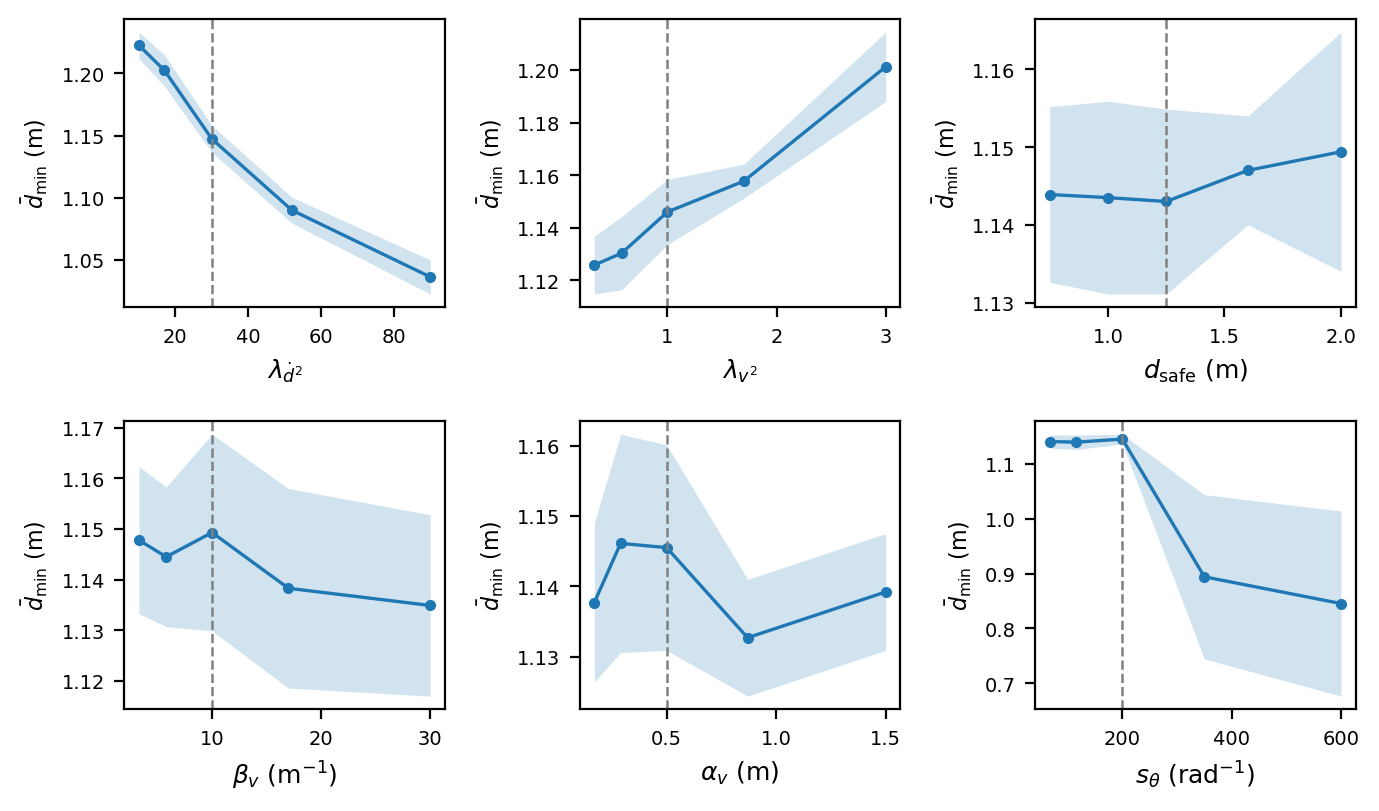
\includegraphics[width=1\columnwidth]{Figures/fig_sensitivity.png}
    \caption[One-at-a-time parameter sensitivity]{One-at-a-time parameter sensitivity of STLMPC over $n=10$ trials per point. Each panel sweeps one parameter ($\lambda_{\dot d^2}$, $\lambda_{v^2}$, $d_\textup{safe}$, $\beta_v$, $\alpha_v$, $s_\theta$) about its nominal value (dashed line); shaded bands show mean~$\pm$~std of the labelled metric. Flat bands indicate robustness.}
    \label{fig:sensitivity}
\end{figure}

\textit{3) Robustness and Baselines:} Table \ref{tab:sim_robust} reports harder scenarios alongside two baselines. Dynamic scenarios use a scripted adversary whose motion violates the constant-velocity/curvature prediction assumption through mid-encounter braking and swerving, and a two-vehicle case in which one adversary is initially occluded; sensor degradation is emulated by elevated scan noise with random beam dropout. The FGM baseline (canonical gap-following, without the tracking-line QP or MPC layers) consequently maintains lower clearance and exhibits larger control effort, quantifying the benefit of those layers. Under adversary maneuvers that break the prediction model, the minimum TTC degrades gracefully rather than collapsing, as the clearance-maximizing tracking lines and supervisory stop provide a fallback margin. To assess generalization beyond the maps used in the ablations, STLMPC is additionally run on two maps not used in the ablations (Maps~\#3 and~\#5, the latter a forked layout): the success rate remains \TBD\% and \TBD\% with average clearance $\bar d_\textup{min}$ of \TBD~m and \TBD~m, indicating the planner is not tuned to the specific test maps. Per-seed results are provided as supplementary material.

% ==========================================================================
% TABLE \ref{tab:sim_robust} -- fill every \TBD from aggregate_runs.py.
%   minTTC column: from scripts/compute_ttc.py (dynamic runs only); use "---"
%   for static rows (R4 noise, FGM-static). N/A success where all crash.
% Rows: R1/R2/R3 dynamic on Map #2, R4 scan noise+dropout on Map #1,
%       FGM/MPPI/SQP baselines all on Map #4 (racing) for a matched comparison.
% ==========================================================================
\begin{table}[ht]
  \caption{Simulation robustness and baselines (FGM gap-following; MPPI on the identical objective) over $n=10$ randomized trials}
  \label{tab:sim_robust}
  \vspace{-8pt}
  \centering
  \begin{tabular}{l@{\hskip 4pt}c@{\hskip 5pt}c@{\hskip 5pt}c@{\hskip 5pt}c@{\hskip 5pt}c}
    \toprule\\[-0.85em]
    \scriptsize Scenario & \makecell{\scriptsize Success\\(\%)} & \makecell{\scriptsize$\min_{\tilde k} d_{\textup{min},\tilde k}$\\(m)} & \makecell{\scriptsize$\bar{d}_\textup{min}$\\(m)} & \makecell{\scriptsize$\min\textup{TTC}$\\(s)} & \makecell{\scriptsize$\bar{v}_{\textup{cmd}}$\\(m/s)}\\
    \midrule\\[-0.85em]
    \scriptsize R1: adversary brakes & \TBD & \TBD & \TBD & \TBD & \TBD \\
    \scriptsize R2: adversary swerves & \TBD & \TBD & \TBD & \TBD & \TBD \\
    \scriptsize R3: two veh., occluded & \TBD & \TBD & \TBD & \TBD & \TBD \\
    \scriptsize R4: scan noise + dropout & \TBD & \TBD & \TBD & --- & \TBD \\
    \midrule\\[-0.85em]
    \scriptsize FGM baseline (Map \#4) & \TBD & \TBD & \TBD & --- & \TBD \\
    \scriptsize MPPI, same obj. (Map \#4) & \TBD & \TBD & \TBD & --- & \TBD \\
    \scriptsize STLMPC-SQP (Map \#4) & \TBD & \TBD & \TBD & --- & \TBD \\
    \bottomrule
  \end{tabular}
\end{table}

\textit{4) Solver Choice and Statistics:} Aggregated over all simulation trials, the SLSQP optimization converges in a mean (max) of \TBD~(\TBD) iterations, times out at the $50$~ms limit in \TBD\% of control steps, and reduces the objective from the Algorithm~\ref{algo2} initial guess to the converged solution by a mean ratio $\bar J_\textup{final}/\bar J_\textup{init}=\TBD$. These figures substantiate the claim that the feasible initial guess places the solver near a low-cost local optimum and that the feasibility-preserving timeout maintains the real-time control rate. To assess whether the SQP choice or its local solutions are a limiting factor, a sampling-based Model Predictive Path Integral (MPPI) optimizer is run on the \emph{identical} formulation---the same objective and the same constraints, imposed as quadratic penalties over kinematically-rolled-out samples---as a solver-only substitution on the racing map (Table \ref{tab:sim_robust}). With $\TBD$ rollouts per step, MPPI reaches a converged objective within \TBD\% of the SQP solution and comparable obstacle clearance, indicating that the SQP local optimum lies close to the broadly-sampled optimum for this problem and is therefore not a meaningful limitation. This comparison isolates solution quality on a common formulation, not implementation efficiency: a parallelized MPPI can achieve high control rates \cite{Williams2016}, while the analytical-gradient SQP used here already satisfies the 10~Hz control rate on the embedded platform. SQP is thus an effective and real-time-capable choice for this problem, rather than a uniformly faster one.


\subsection{Navigation in a Static, Unknown Environment}\label{sec:exp1}
The simulation findings are now validated in real-world conditions on the 1/10$^{\text{th}}$-scale vehicle, across the three physical courses shown in Fig.~\ref{CourseLayouts}. In the first environmental configuration (Experiment~\#1), Section~\ref{sec3}'s STLMPC is evaluated on the static course (Fig.~\ref{CourseLayouts1}) using the parameter values consolidated in Table~\ref{tab:params}, with $n_\textup{MPC}=2$ and $k_\textup{MPC}=8$ creating a receding prediction time horizon of 1.6~s at constant $v=1.5$ m/s.

\begin{figure*}[!t]
  \centering
  \subfloat[]{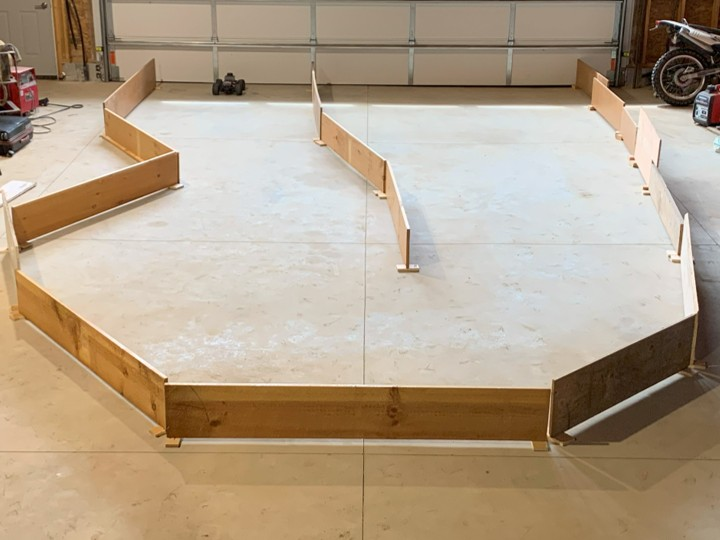
\includegraphics[width=0.24\textwidth]{Figures/ExperimentMap1CROPPED.jpg}\label{CourseLayouts1}} \hfil
  \subfloat[]{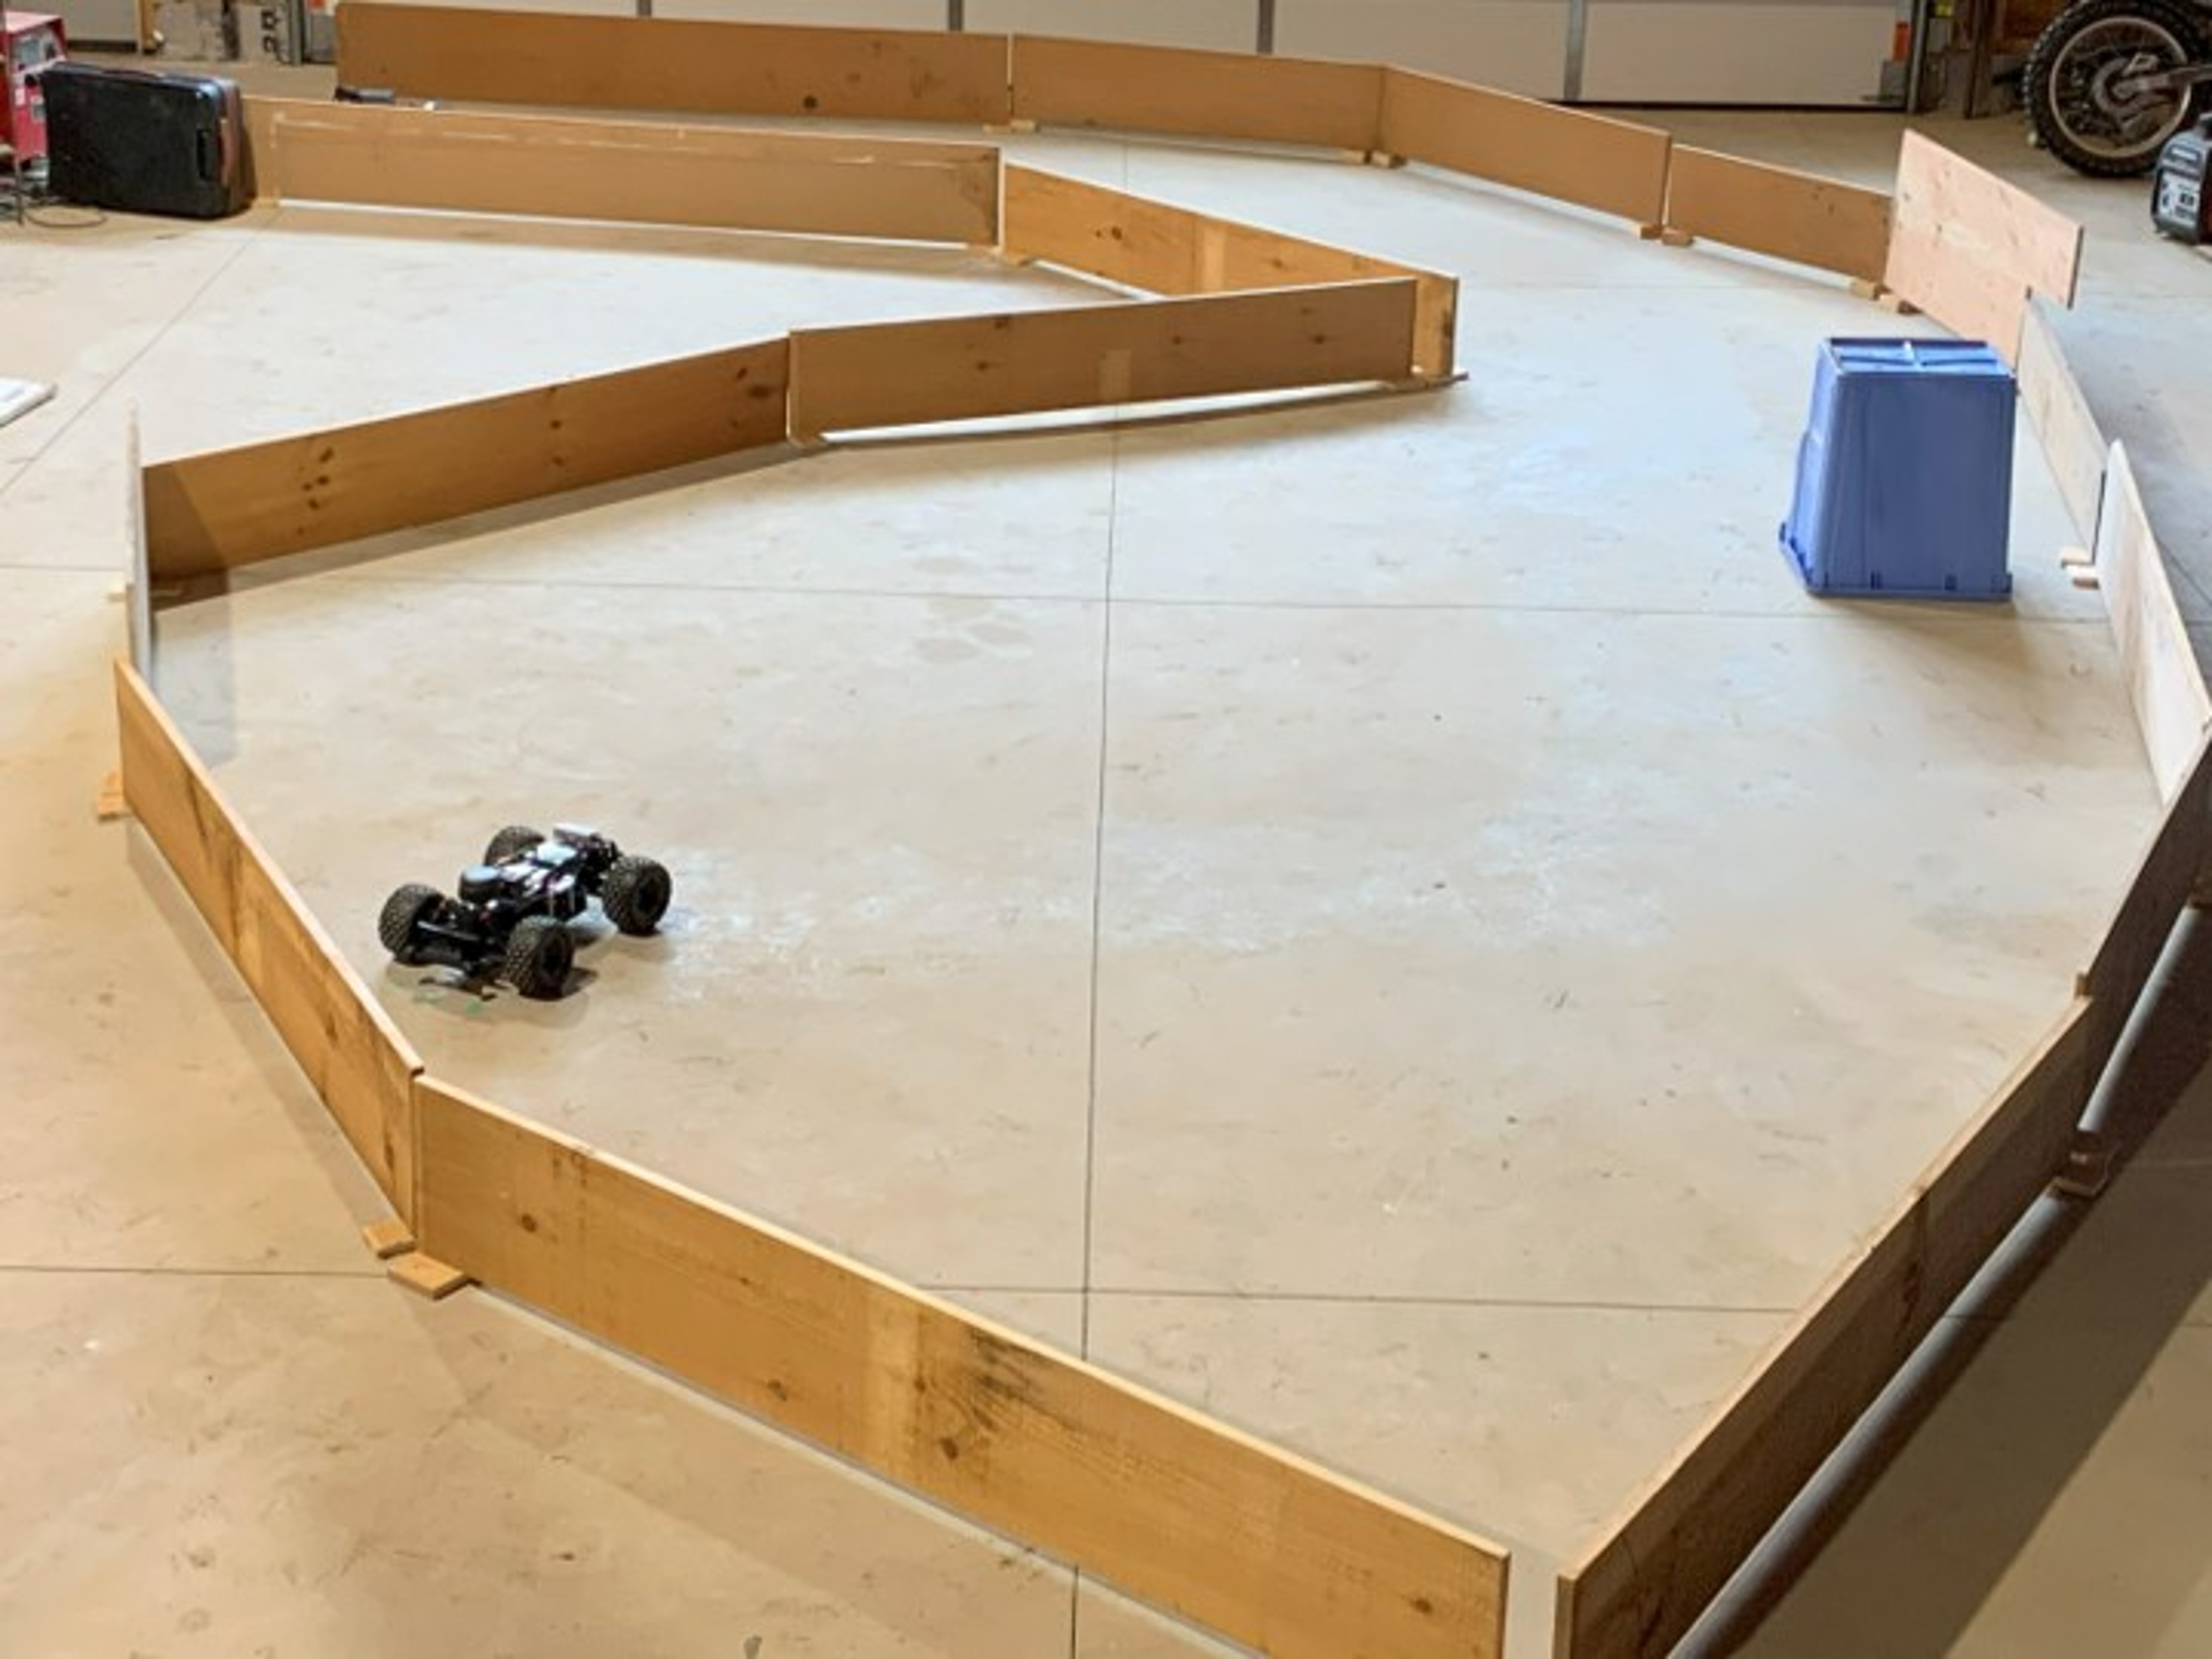
\includegraphics[width=0.24\textwidth]{Figures/ExperimentMap2CROPPED.jpg}\label{CourseLayouts2a}} \hfil
  \subfloat[]{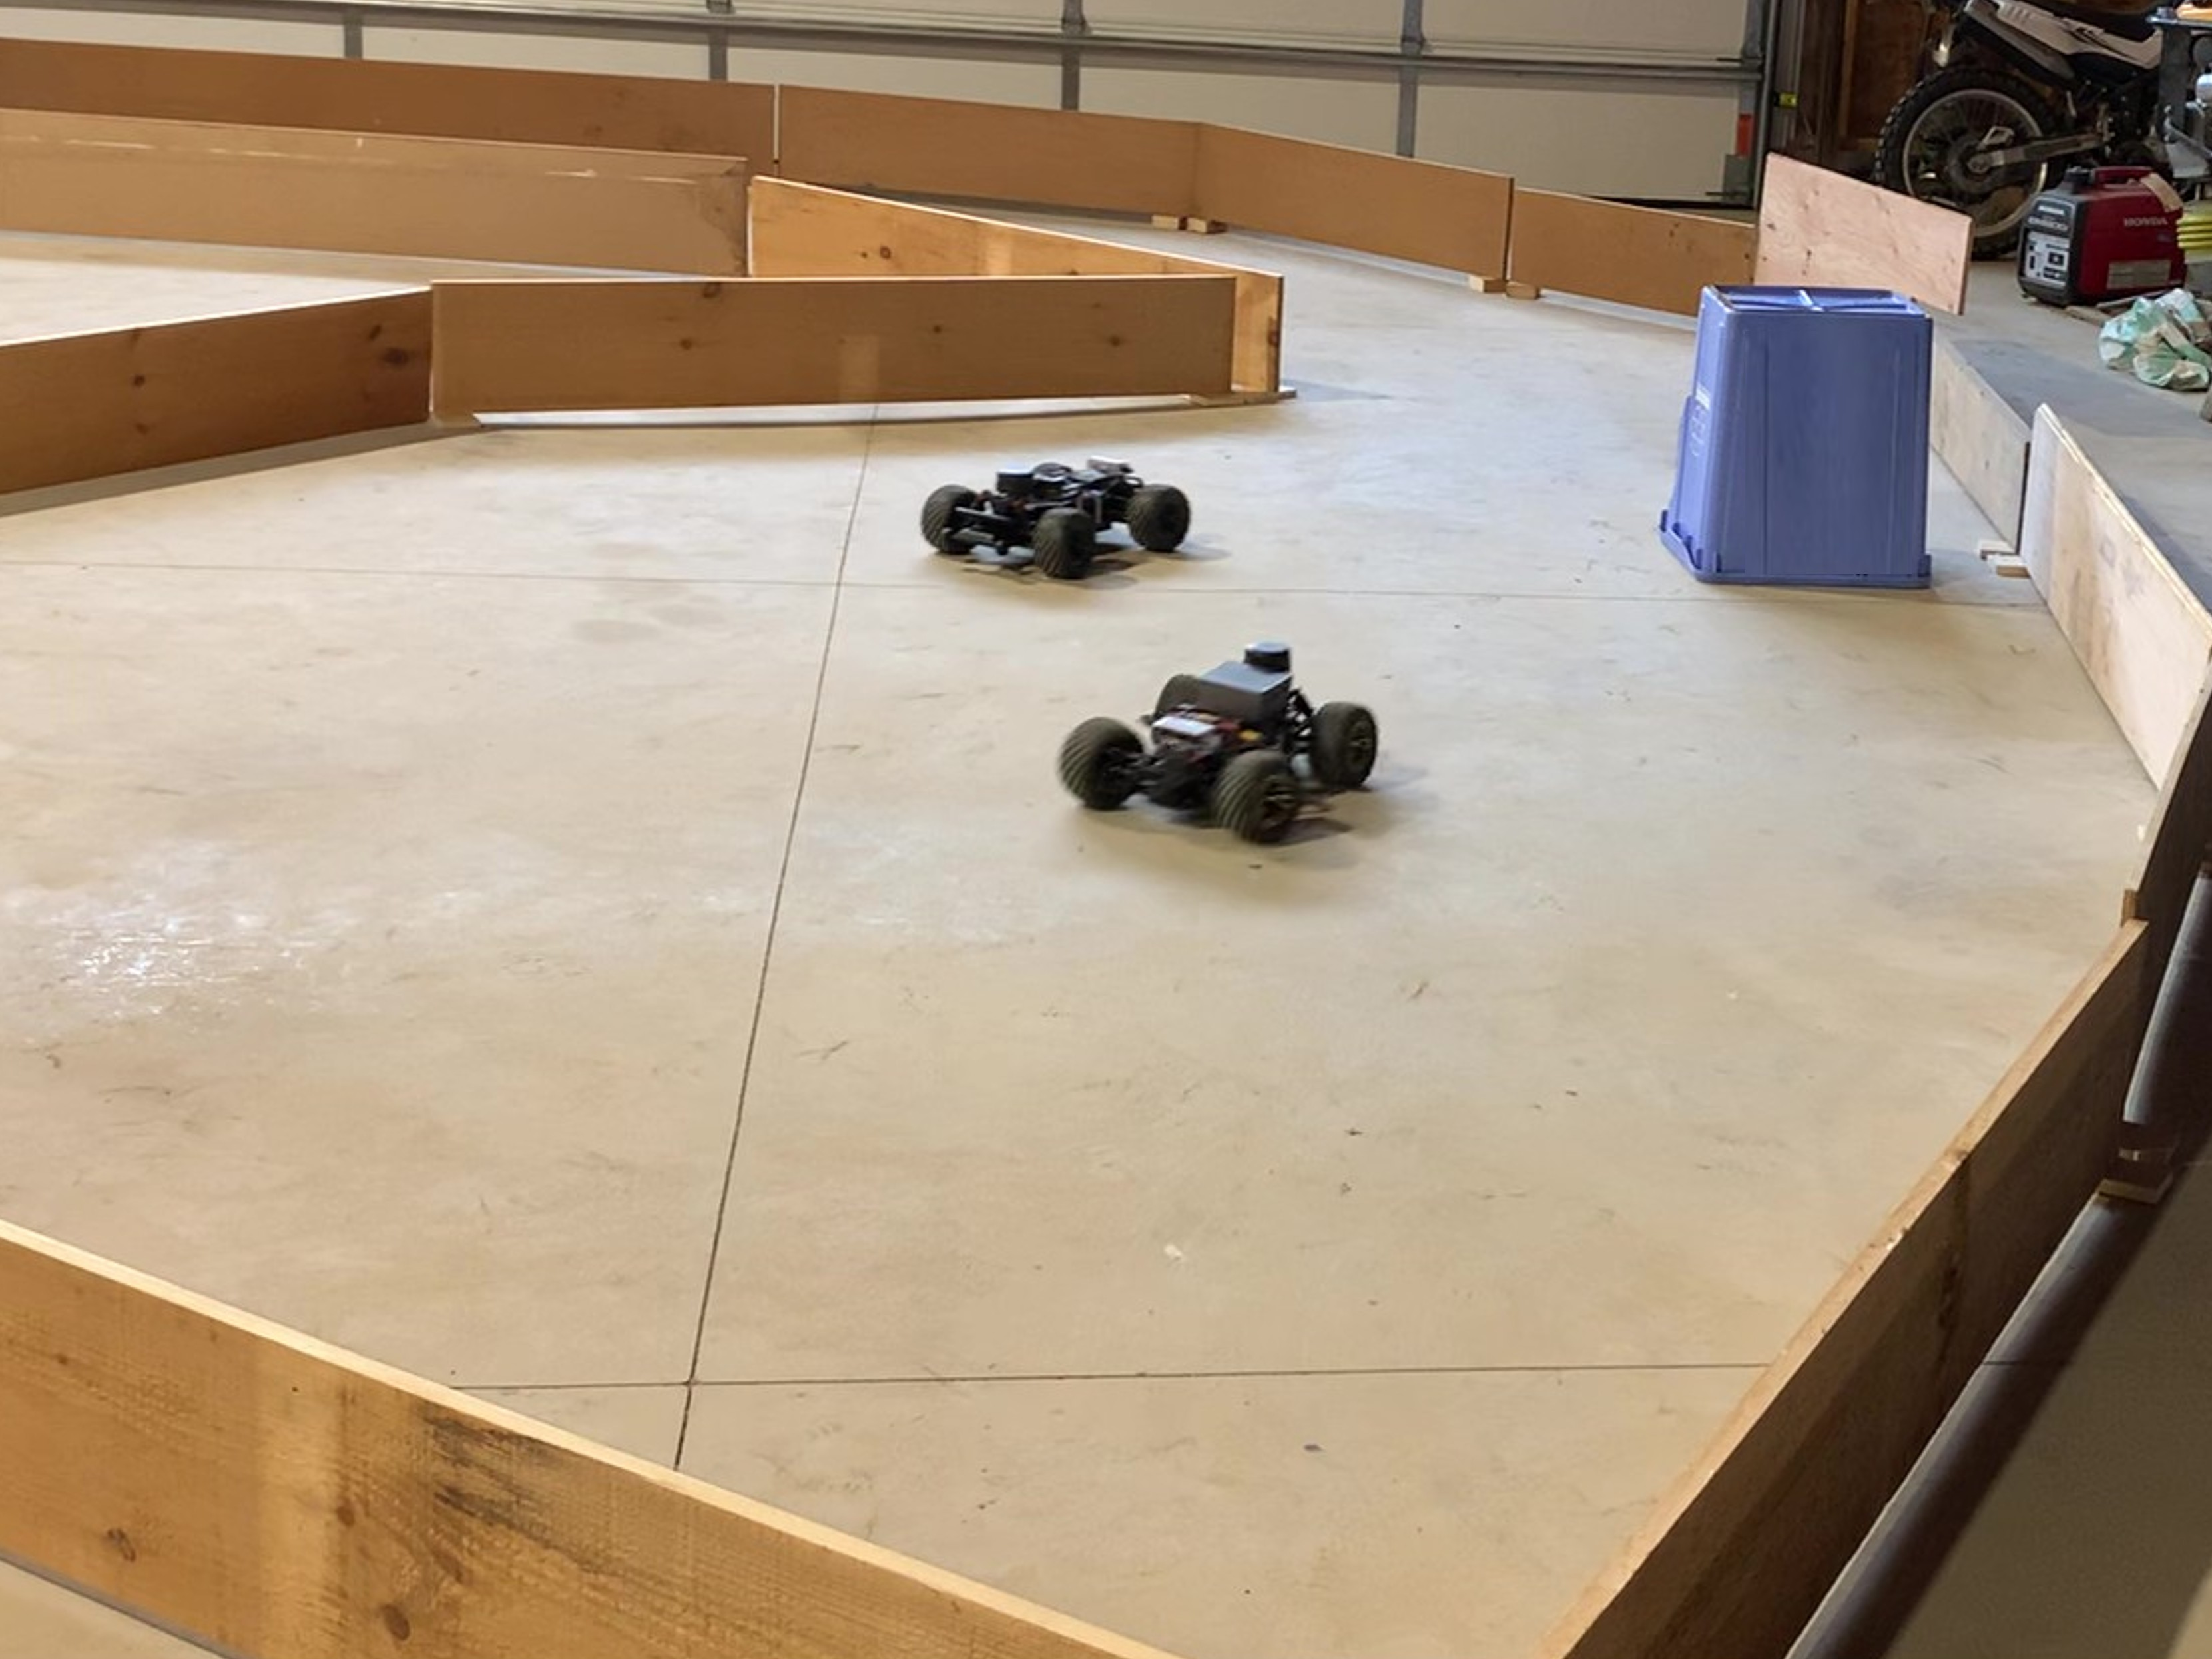
\includegraphics[width=0.24\textwidth]{Figures/ANON2_Experiment_Dynamic_Frame.jpg}\label{CourseLayouts2b}}
  \hfil
  \subfloat[]{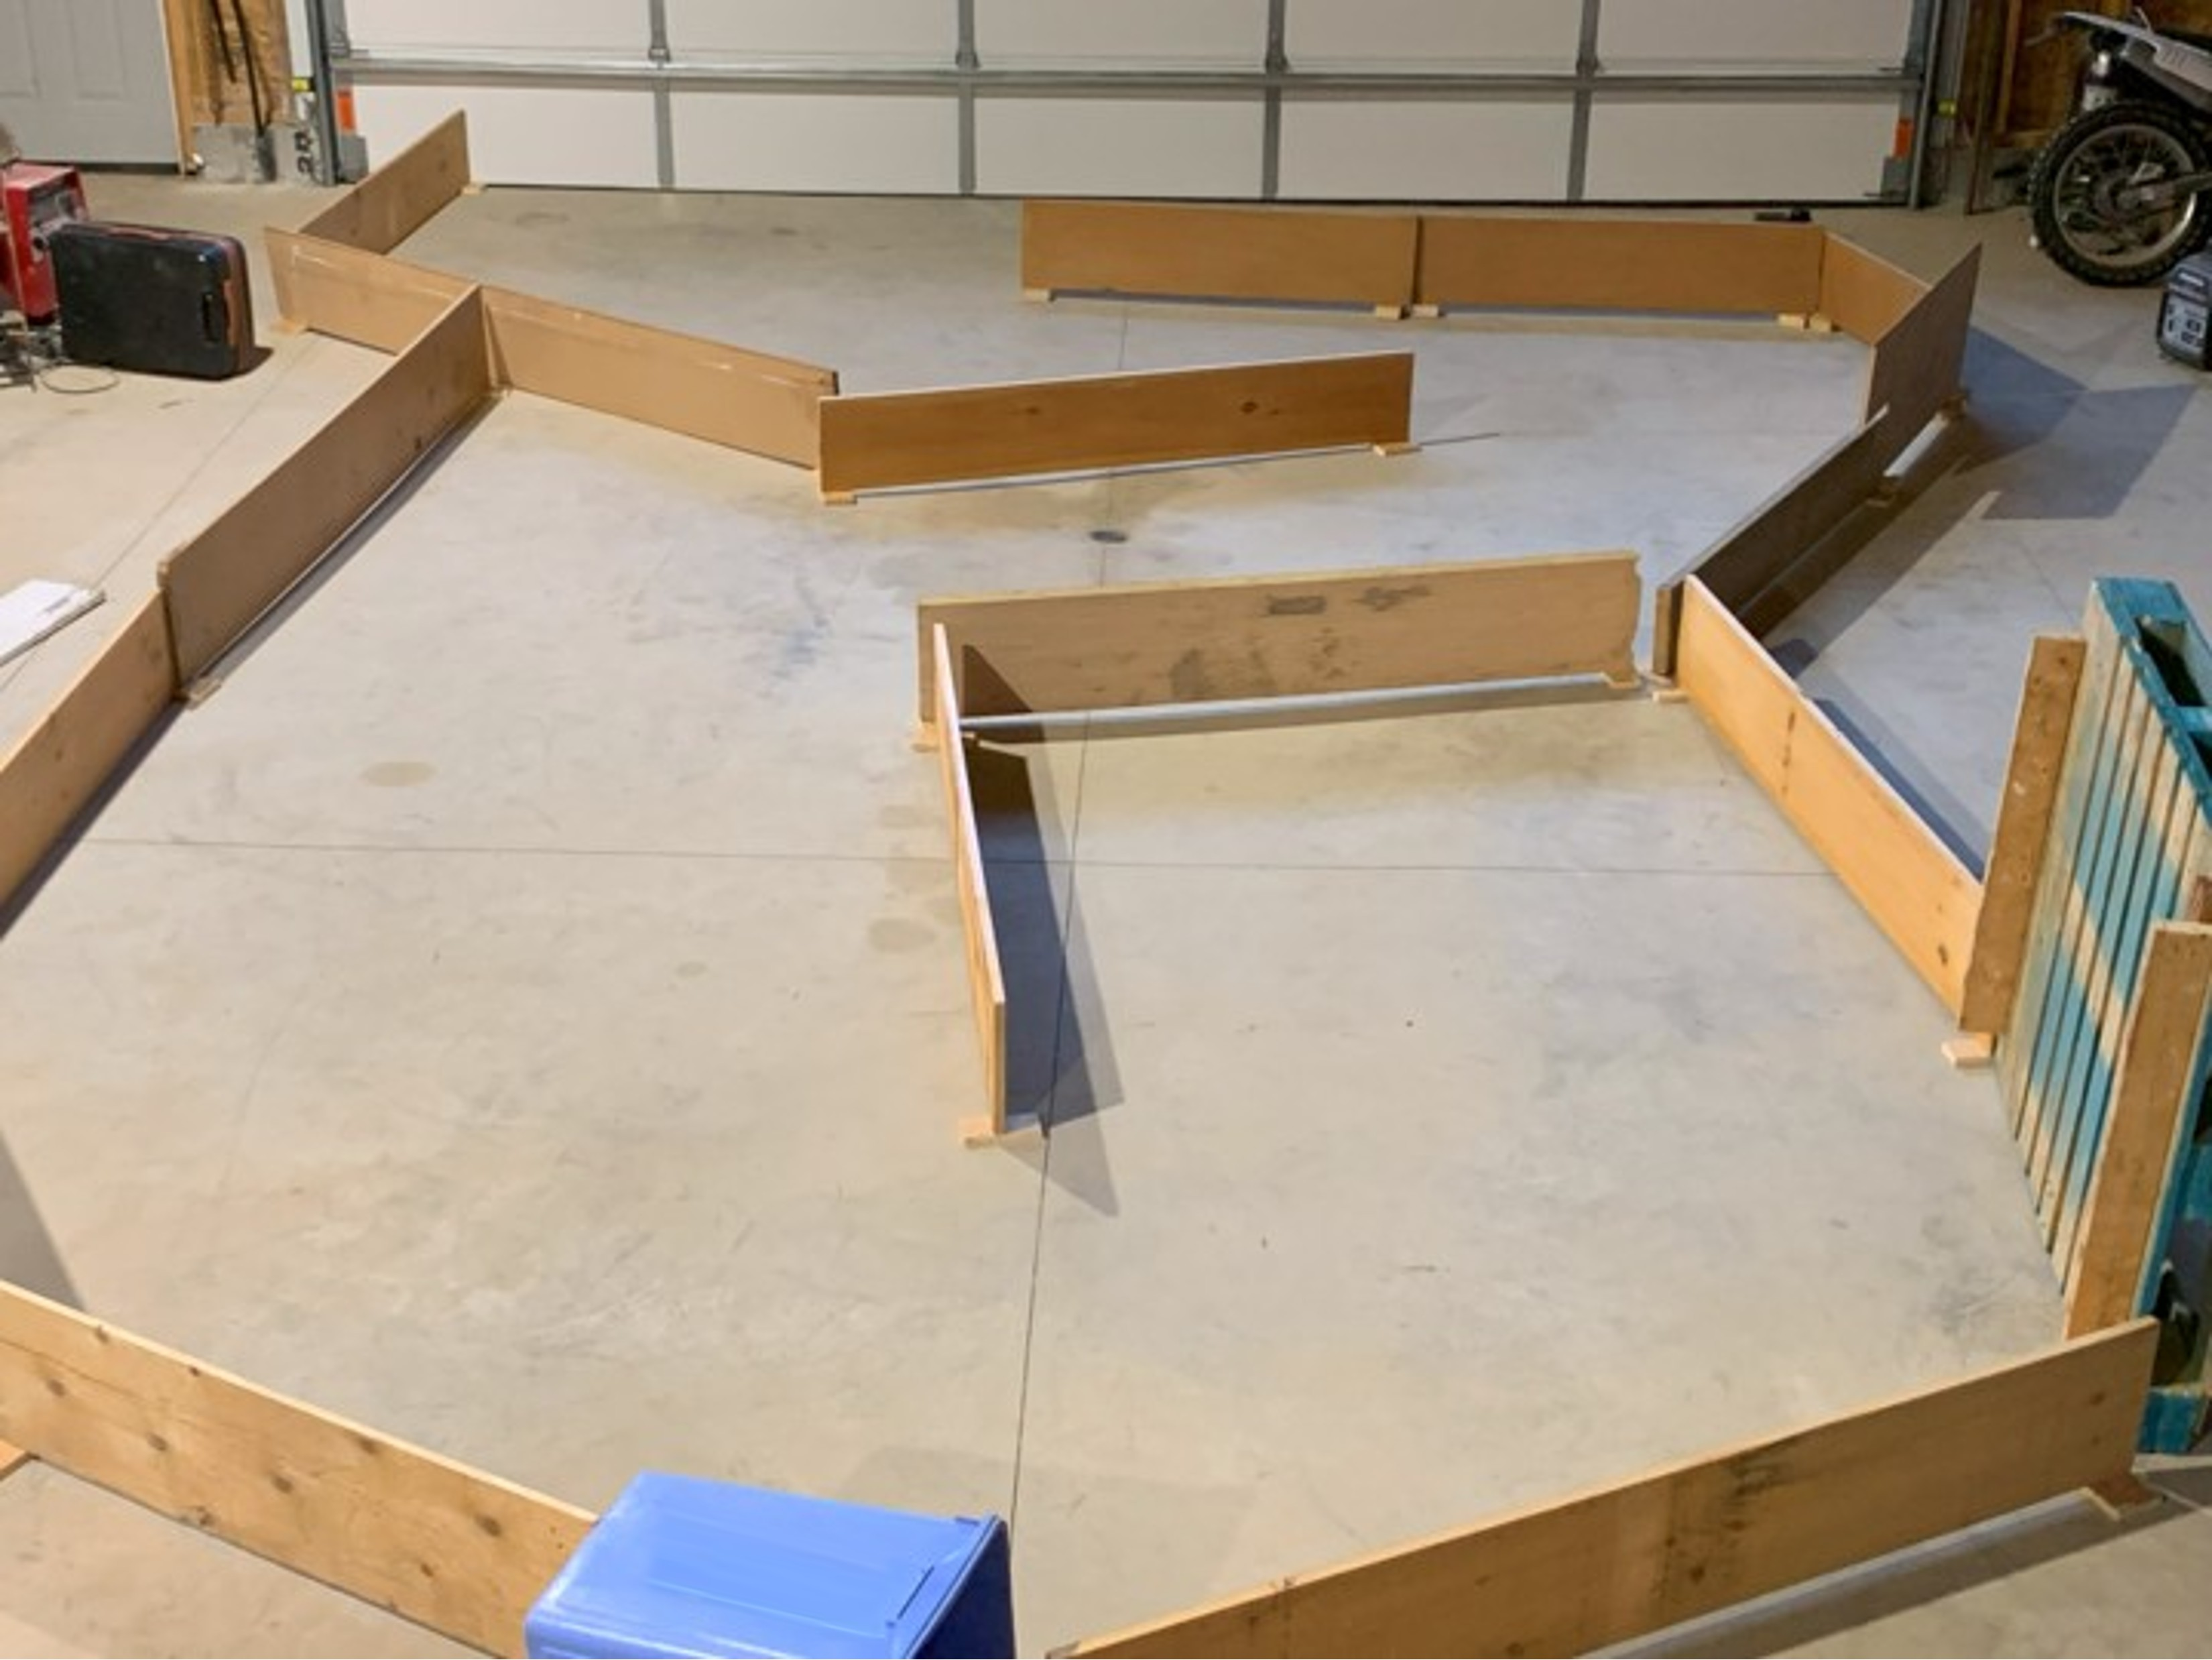
\includegraphics[width=0.24\textwidth]{Figures/ExperimentMap3IMAGE.jpg}\label{CourseLayouts3}}
  \caption[Physical course layouts for the hardware experiments]{The three physical courses used for the hardware experiments: (a) the static course (Experiment~\#1); (b) before and (c) after dynamic vehicle avoidance (Experiment~\#2); and (d) the racing course (Experiment~\#3). The simulation studies use a separate set of simulator maps.}
    \label{CourseLayouts}
\end{figure*}

Performance is assessed in real-world conditions for the DWA, TEB and MPC exploration-based methods, the PD approach, Section \ref{sec3}'s STLMPC and AMCL-localized STLMPC using an occupancy grid map. Fig. \ref{chap3exp} shows the path of each local planner, where both STLMPC planners effectively maintain paths near the center of the course, maximizing obstacle clearance. Although the AMCL-localized planner obtains a longer effective look-ahead horizon, differences in closed-loop performance between the STLMPC methods are negligible. The value of the tracking line approach is shown as PD achieves a central path similar to STLMPC, whereas the exploration methods do not, risking collision. Of the exploration local planners, TEB is most effective where DWA progresses at a lower speed than desired and MPC oscillates unexpectedly due to occasional poor optimization solutions.

\begin{figure}[ht]
    \centering
    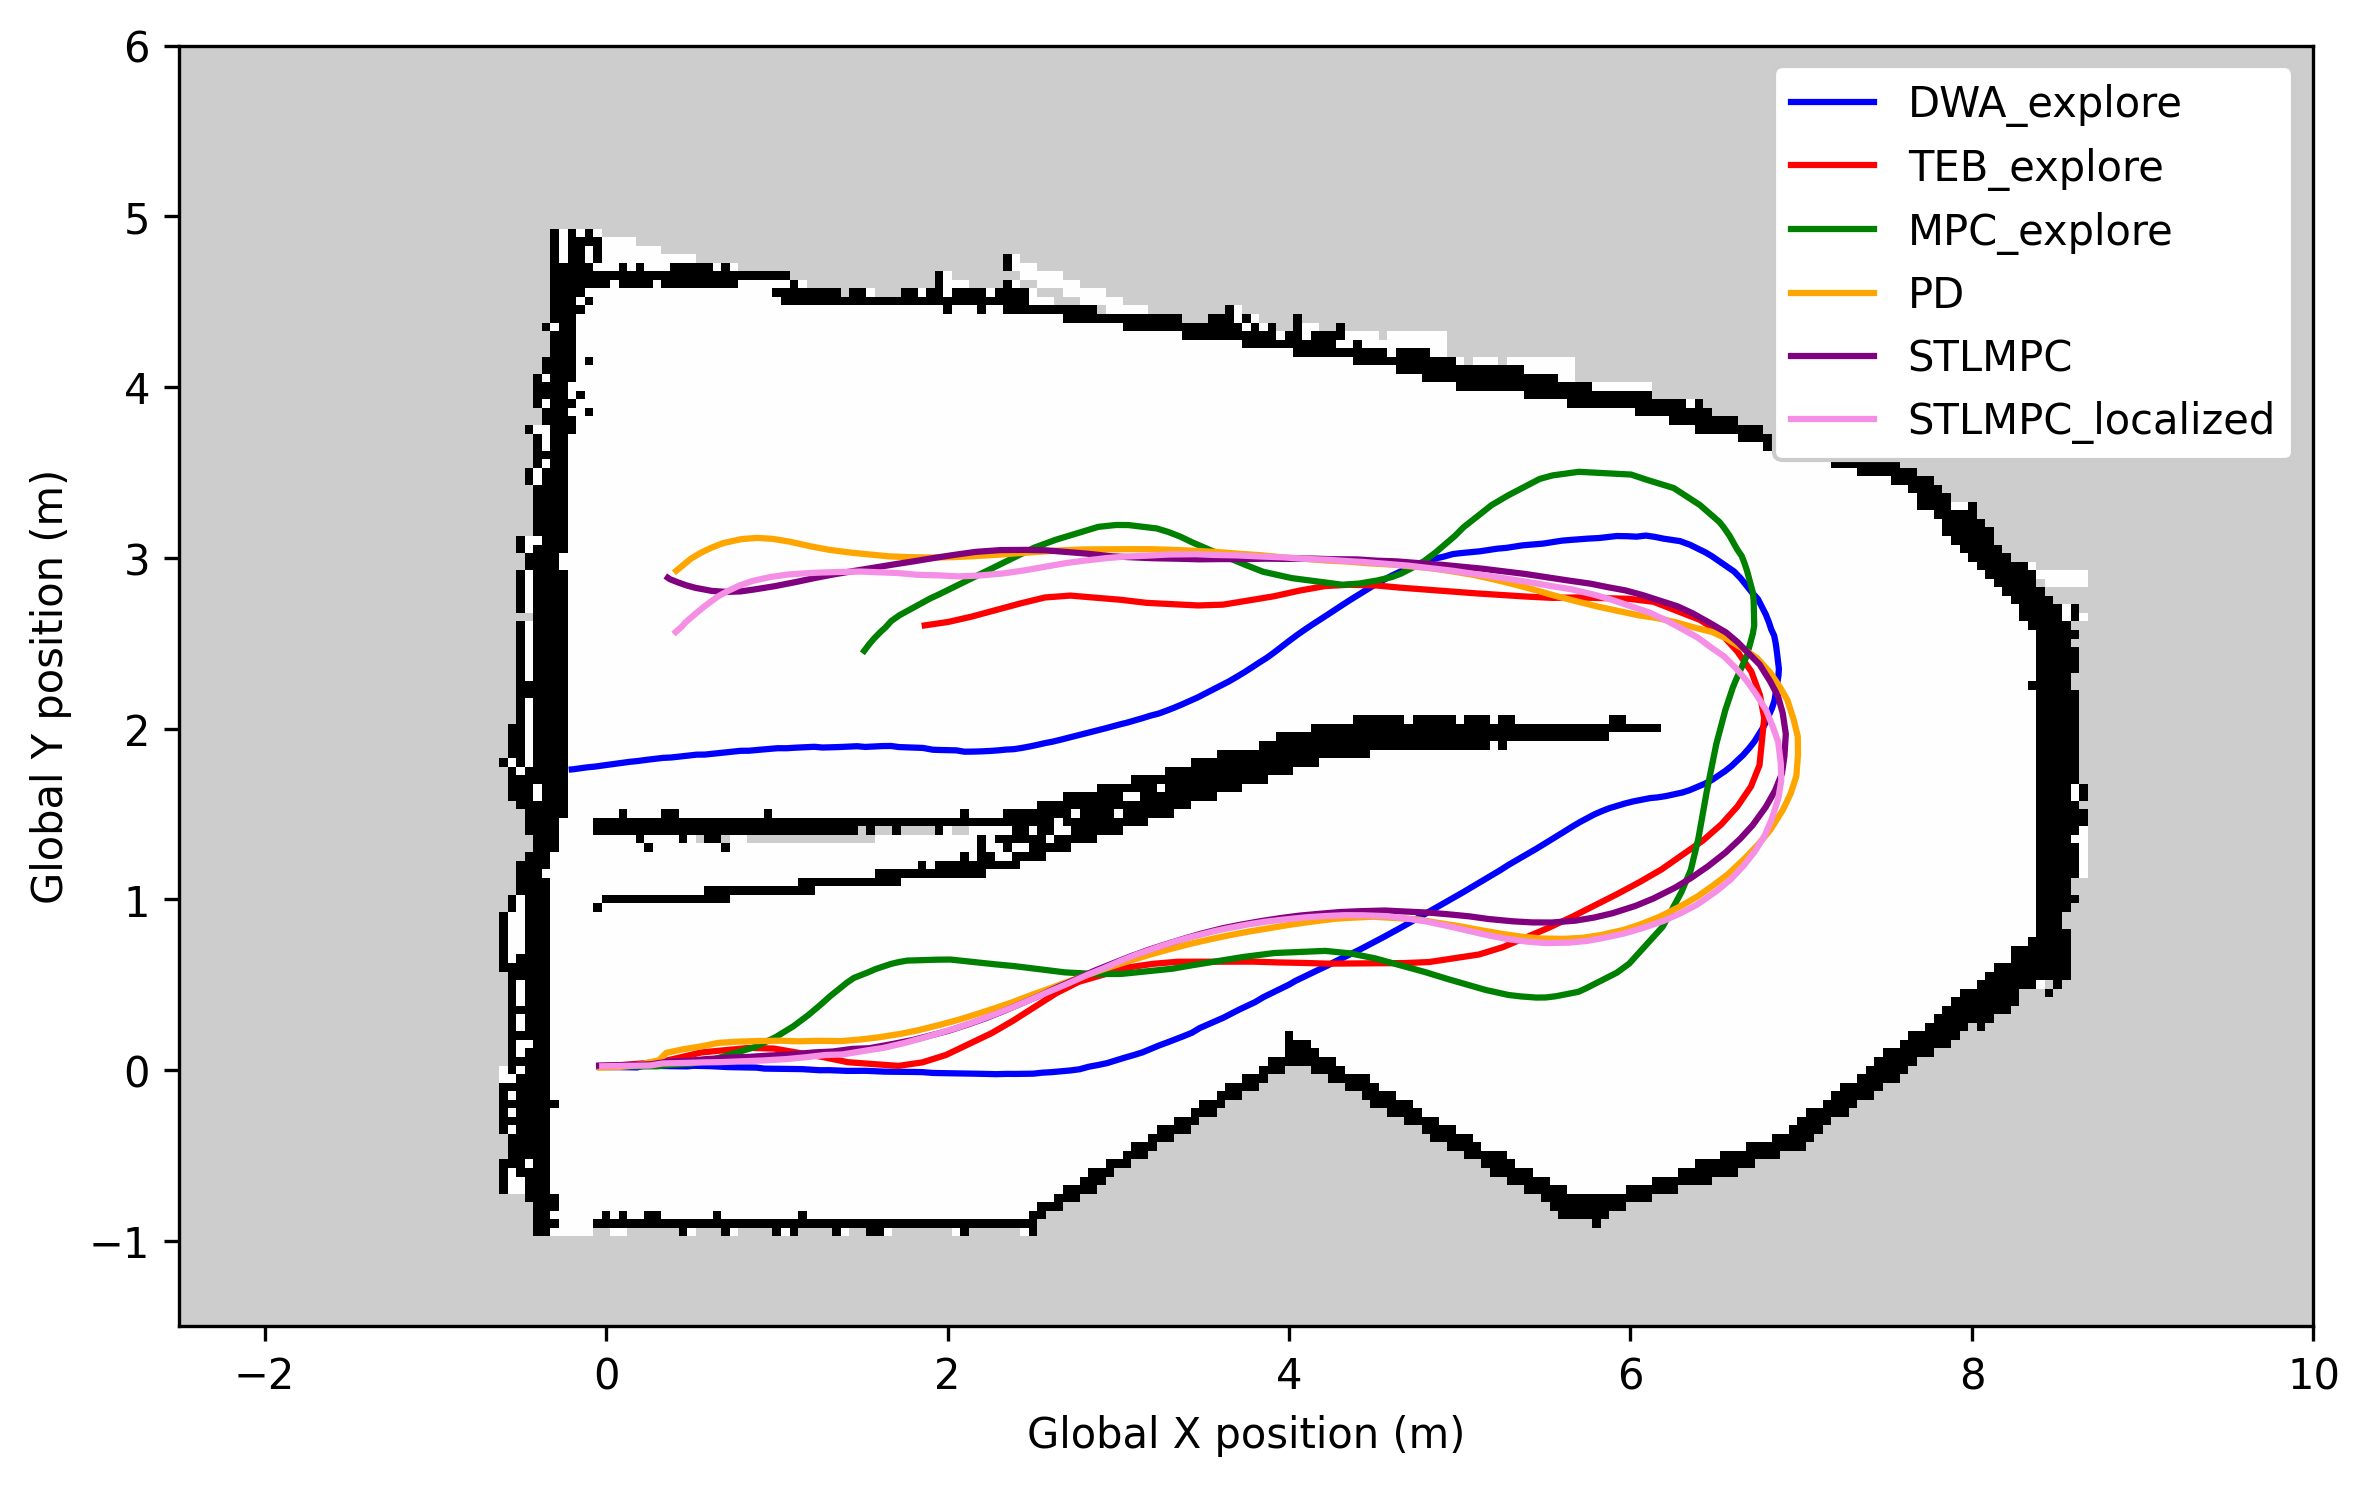
\includegraphics[width=0.86\columnwidth]{Figures/Exp3TrajsShorter.png}
    \caption[Path trajectories for all compared local planners in Experiment \#1]{Paths obtained by each local planner in Experiment \#1. Each path starts at the global origin and proceeds counterclockwise around the map.}
	\label{chap3exp}
\end{figure}

Key metrics for planner performance are quantified for the\vspace{1pt} first experiment in Table \ref{tab:STLMPCexp3}, using the proximity and control-input measures defined in Section \ref{sec:simstudies} (with $\tilde k$ ranging over the full test). The STLMPC methods perform best in terms of the obstacle proximity metrics while also exhibiting low control effort and attaining an average velocity near the desired 1.5 m/s speed. Here, PD performs comparably to STLMPC, although marginally worse, while the TEB local planner achieves the best performance among the exploration-based approaches.

\begin{table}[ht]
  \caption{Performance of local planners including STLMPC in Experiment \#1}
  \label{tab:STLMPCexp3}
  \vspace{-8pt}
  \centering
  \begin{tabular}{l@{\hskip 3.4pt}c@{\hskip 4pt}c@{\hskip 6pt}c@{\hskip 5pt}c@{\hskip 4pt}c@{\hskip 4pt}c}
    \toprule\\[-0.85em]
    \scriptsize Local Planner & \makecell{\scriptsize$\min_{\tilde k} d_{\textup{min},\tilde k}$\\[0.2em](m)} & \makecell{\scriptsize$\bar{d}_\textup{min}$\\[0.3em](m)} & \makecell{\scriptsize$\overline{|\delta_{\textup{cmd},\tilde k}|}$\\[0.2em](rad)} & \makecell{\scriptsize$\mathrm{Var}(\delta_{\textup{cmd},\tilde k})$\\[0.2em]($\textup{rad}^2$)} & \makecell{\scriptsize$\bar{v}_{\textup{cmd},\tilde k}$\\[0.3em](m/s)} & \makecell{\scriptsize$\mathrm{Var}(v_{\textup{cmd},\tilde k})$\\[0.2em]($\textup{m}^2$/$\textup{s}^2$)}\\
    \midrule\\[-0.85em]
    \scriptsize DWA\_explore      & 0.385 & 0.654 & 0.118 & 0.028 & 0.491 & 0.012 \\
    \scriptsize TEB\_explore     & 0.570 & 0.843 & 0.157 & 0.032 & 1.356 & 0.139  \\
    \scriptsize MPC\_explore   & 0.313 & 0.831 & 0.253 & 0.073 & 0.858 & 0.149  \\
    \scriptsize PD   & 0.587 & 0.978 & 0.147 & 0.032 & 1.281 & 0.107  \\
    \scriptsize STLMPC   & 0.688 & 0.972 & 0.113 & 0.025 & 1.304 & 0.071  \\
    \scriptsize STLMPC\_loc   & 0.640 & 0.982 & 0.116 & 0.019 & 1.296 & 0.065  \\
    \bottomrule
  \end{tabular}
\end{table}

Furthermore, each planner's computation time ($t_{\textup{comp},\tilde k}$) is compared in both the average ($\bar{t}_\textup{comp}$) and worst ($\displaystyle\max t_\textup{comp}$) case via Table \ref{tab:STLMPCcomp3}. Here, the exploration-based planners have three planning stages: updating unexplored frontiers and setting a new goal, global planning to this goal and finally, local planning to track this path while performing collision avoidance. The methods differ in the third stage where the computation times for each step are denoted by $t_{\textup{frn},\tilde k},\,t_{\textup{glb},\tilde k}\ \& \ t_{\textup{loc},\tilde k}$ respectively and summed for the total planning time $t_{\textup{comp},\tilde k}$.

The simplistic PD approach achieves the lowest average computation time, while STLMPC also attains reliably low planning times. The choice of prediction horizon length ($n_\textup{MPC}k_\textup{MPC}$) directly impacts optimization complexity and computation time. The computational performance of STLMPC and TEB is comparable in this experiment, while the use of AMCL has minimal impact on computation time. MPC-based exploration has significantly longer planning times, far exceeding the 100-ms control period in the worst case.

\begin{table}[ht]
\caption{Planning computation times for local planners including STLMPC in Experiment \#1}
\label{tab:STLMPCcomp3}
\vspace{-8pt}
\centering
\begin{tabular}{
    l@{\hskip 3.4pt}c@{\hskip 4.0pt}c@{\hskip 4.0pt}c@{\hskip 5.5pt}c@{\hskip 3.2pt}c@{\hskip 3.2pt}c@{\hskip 3.2pt}c@{\hskip 3.2pt}c
}
\toprule\\[-1.2em]
\scriptsize Local Planner &
\makecell{\scriptsize$\bar{t}_\textup{frn}$\\(ms)} &
\makecell{\scriptsize$\bar{t}_\textup{glb}$\\(ms)} &
\makecell{\scriptsize$\bar{t}_\textup{loc}$\\(ms)} &
\makecell{\scriptsize\bm{$\bar{t}_\textbf{comp}$}\\\textbf{(ms)}} &
\makecell{\scriptsize$\max t_\textup{frn}$\\(ms)} &
\makecell{\scriptsize$\max t_\textup{glb}$\\(ms)} &
\makecell{\scriptsize$\max t_\textup{loc}$\\(ms)} &
\makecell{\scriptsize$\bm{\max t_\textbf{comp}}$\\\textbf{(ms)}} \\
\midrule\\[-1.2em] 
{\scriptsize DWA\_explore} & 3.6 & 0.9 & 11.8 & \textbf{16.3} & 7.4 & \phantom{0}1.9 & \phantom{0}27.9 & \phantom{0}\textbf{37.1}  \\
{\scriptsize TEB\_explore} & 1.9 & 0.8 & \phantom{0}3.2 & \phantom{0}\textbf{5.9} & 5.2 & \phantom{0}1.5 & \phantom{00}8.3 & \phantom{0}\textbf{15.0}  \\
{\scriptsize MPC\_explore} & 2.0 & 1.1 & 43.7 & \textbf{46.7} & 3.8 & 10.2 & 484.8 & \textbf{498.8}  \\
{\scriptsize PD} & \multicolumn{3}{c}{~~~} & \phantom{0}\textbf{0.5} & \multicolumn{3}{c}{~~~} & \phantom{00}\textbf{1.7}  \\
{\scriptsize STLMPC} & \multicolumn{3}{c}{~~~} & \phantom{0}\textbf{6.5} & \multicolumn{3}{c}{~~~} & \phantom{0}\textbf{15.8}  \\
{\scriptsize STLMPC\_loc} & \multicolumn{3}{c}{~~~} & \phantom{0}\textbf{6.9} & \multicolumn{3}{c}{~~~} & \phantom{0}\textbf{12.3}  \\
\bottomrule
\end{tabular}
\end{table}

% While the overall performance of STLMPC with and without AMCL-based localization is similar, the effect on path planning at individual iterations is significant. Fig. \ref{STLMPC_AMCLcompare} shows the STLMPC tracking lines and optimized path at a single, shared iteration, both using and not using localized map data. The planner without AMCL does not see around the right wall and therefore plans to turn right, while the AMCL-localized planner uses map data of this unseen area to correctly plan to turn left. In practice, STLMPC without AMCL proceeds along the correct path once it detects the obscured wall, and this deficiency in effective look-ahead horizon leads to negligible differences in performance, as seen in earlier results.



% \begin{figure}[ht]
%   \centering
%     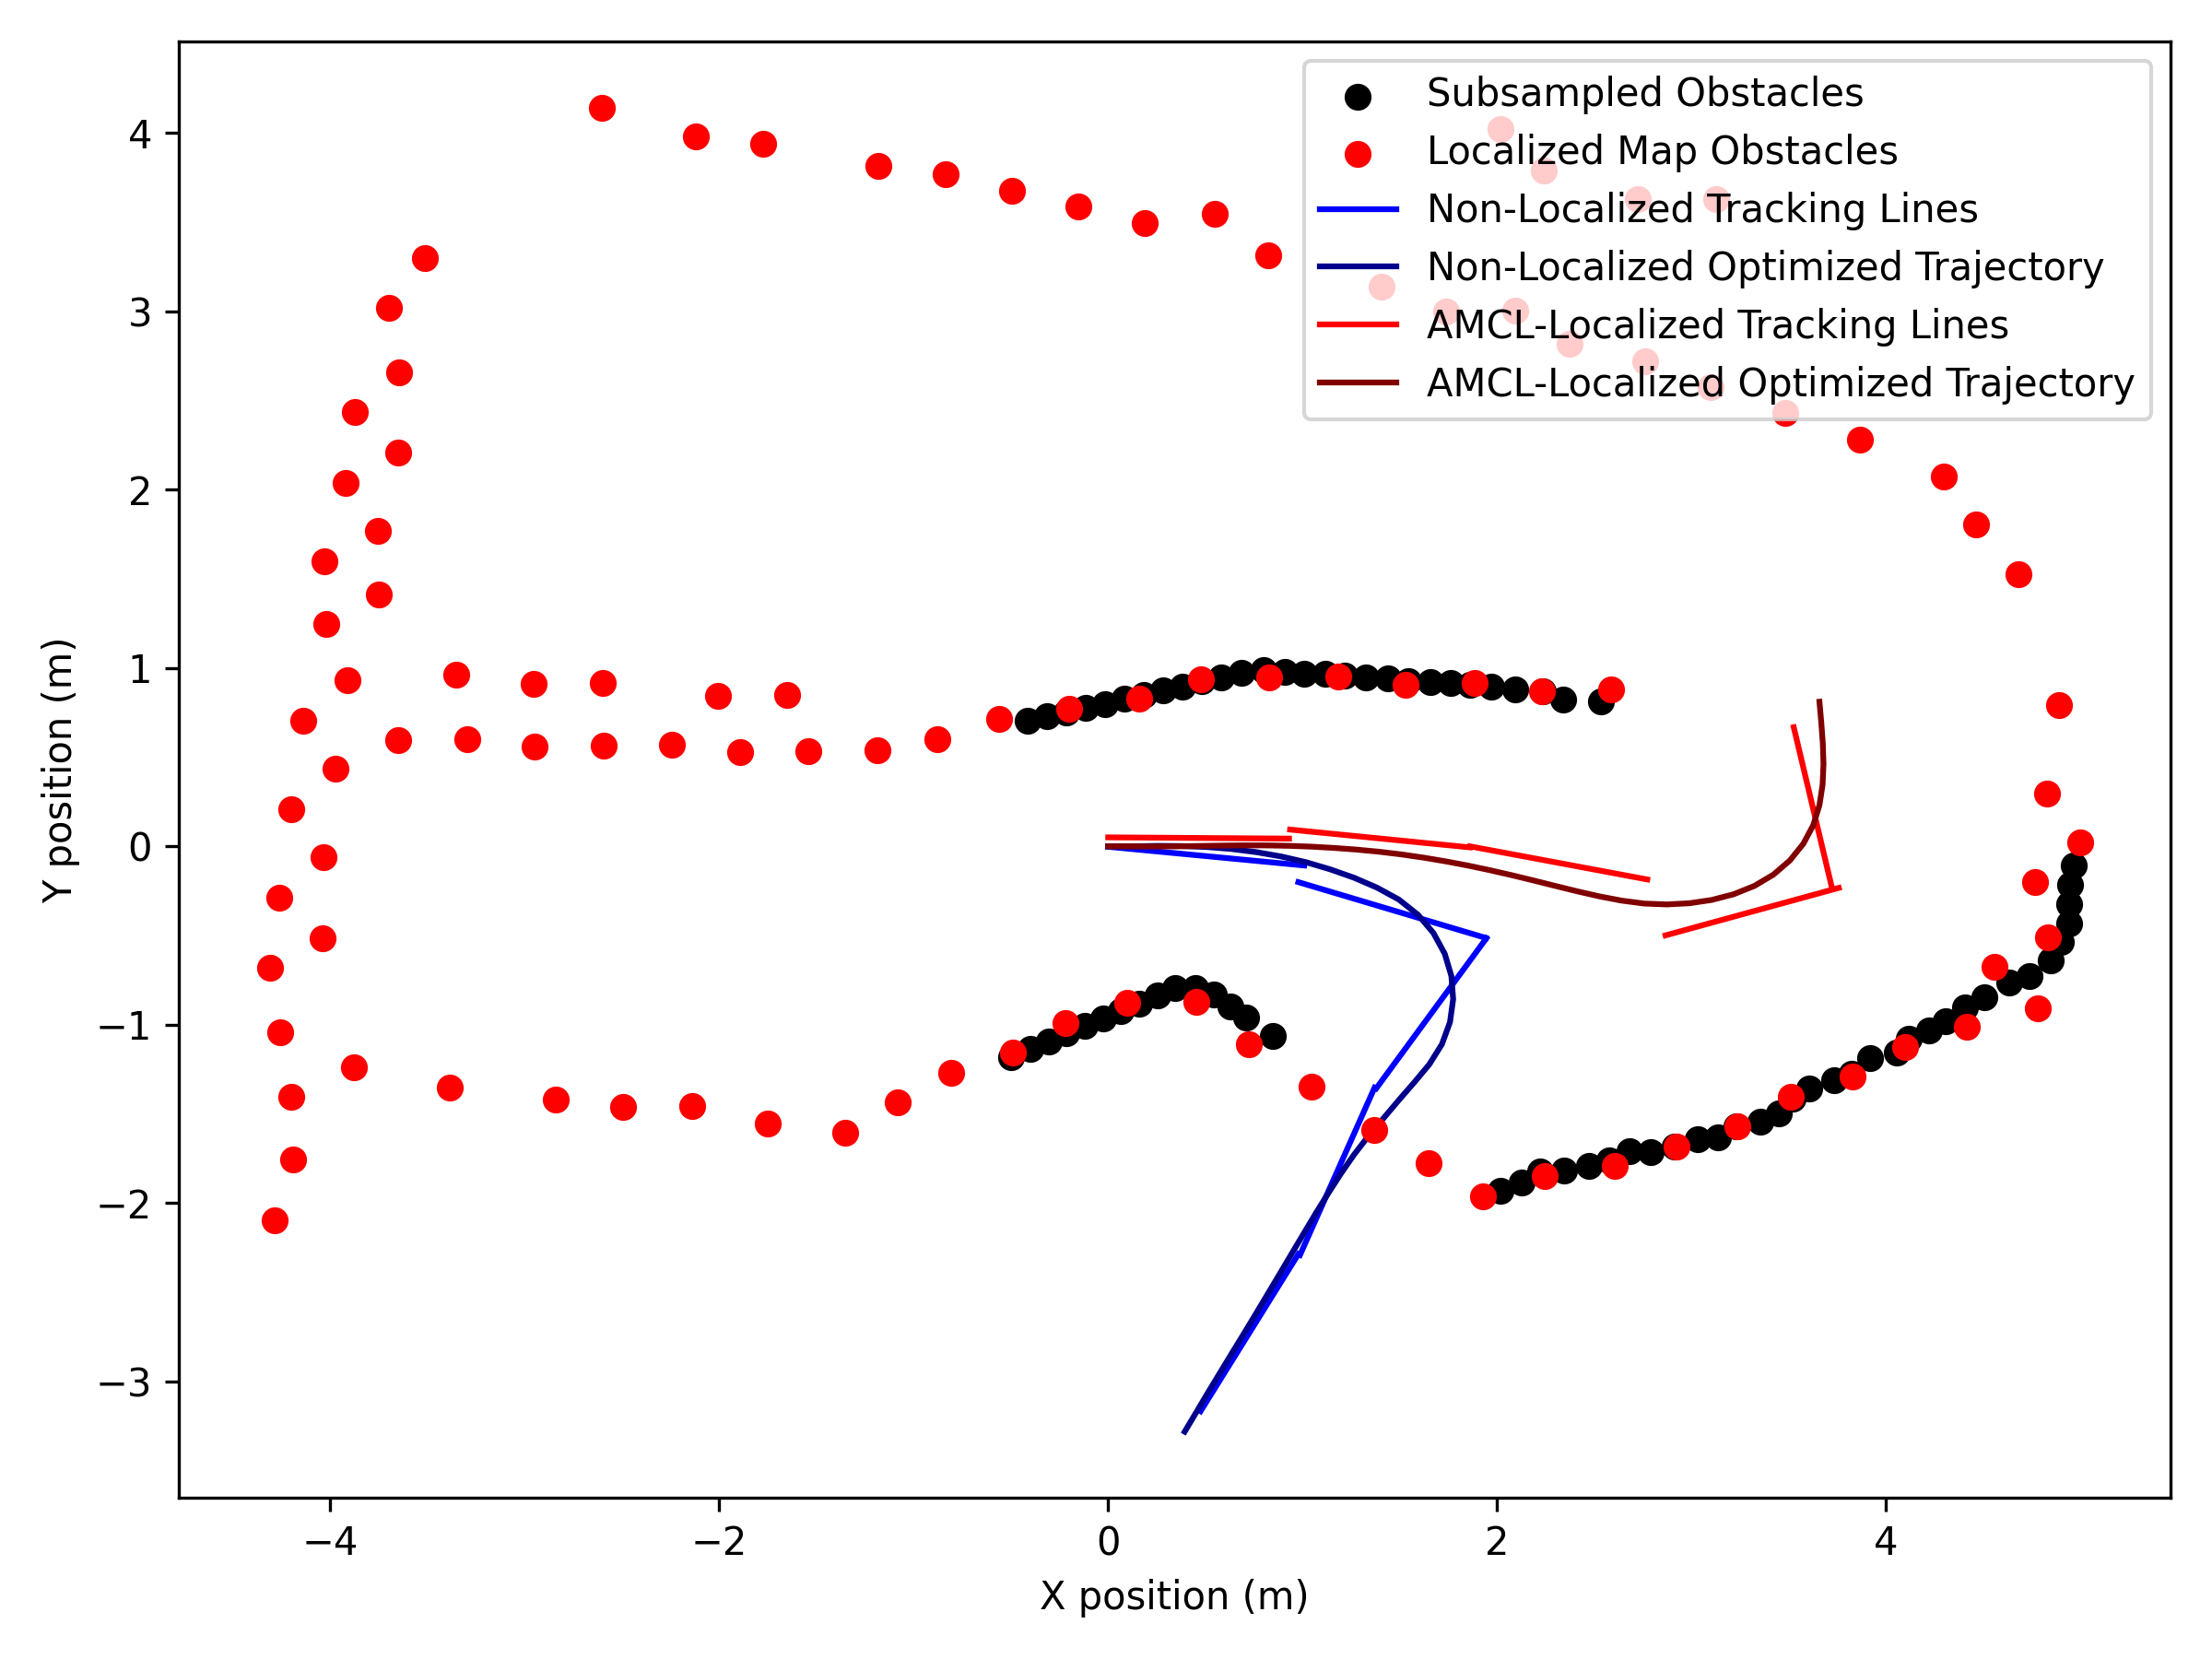
\includegraphics[width=0.78\columnwidth]{Figures/Exp3BothAMCL.png}%
%   \caption[Optimized trajectories at a single iteration for STLMPC with and without AMCL in Experiment \#1]{Tracking lines and optimized trajectory at a shared timestep for STLMPC both with and without AMCL in Experiment \#1.}
%   \label{STLMPC_AMCLcompare}
% \end{figure}

\subsection{Dynamic Vehicle Avoidance Scenario}\label{sec:exp2}
Vehicle detection, tracking and avoidance are now evaluated in a second real-world experiment, Experiment \#2 (Figs. \ref{CourseLayouts2a} and \ref{CourseLayouts2b}). Parameters are reused from the prior experiment, now with $\text{l}_\text{v}=0.5$ m and $\text{w}_\text{v}=0.4$ m. Dynamic obstacle avoidance is tested for Section \ref{sec3}'s STLMPC and TEB-based exploration, which consider all obstacles statically, as well as Section \ref{sec4}'s STLMPC, which incorporates dynamic obstacles. TEB is used in this experiment as the best-performing exploration approach from prior tests. Each planner's trajectory is provided in Fig. \ref{Chap4expavoid} alongside that of the detected vehicle, where the TEB-based planner takes minimal action to avoid the adversarial vehicle. Section \ref{sec3}'s STLMPC swerves slightly while Section \ref{sec4}'s STLMPC makes the most significant maneuver to avoid the tracked vehicle, ensuring safety. At a time sample before vehicle avoidance, it is shown how dynamic obstacle STLMPC maintains the greatest clearance from the oncoming vehicle.

The performance metrics for each tested planner are shown in Table \ref{tab:STLMPCexp4}. Dynamic obstacle STLMPC performs best in terms of obstacle proximity, with static obstacle STLMPC performing similarly until vehicle avoidance. All planners exhibit similar control efforts, where the vehicle avoidance maneuver causes larger average steering angle magnitudes for the STLMPC methods. Table \ref{tab:STLMPCcomp4} contains the computation times for each planner, where performance is similar. Average computation times are low for all methods, while static obstacle STLMPC has the lowest worst-case time. Dynamic obstacle STLMPC has the poorest worst-case time, occurring during vehicle avoidance, as the optimization is more difficult.

\begin{figure}[ht]
    \centering
    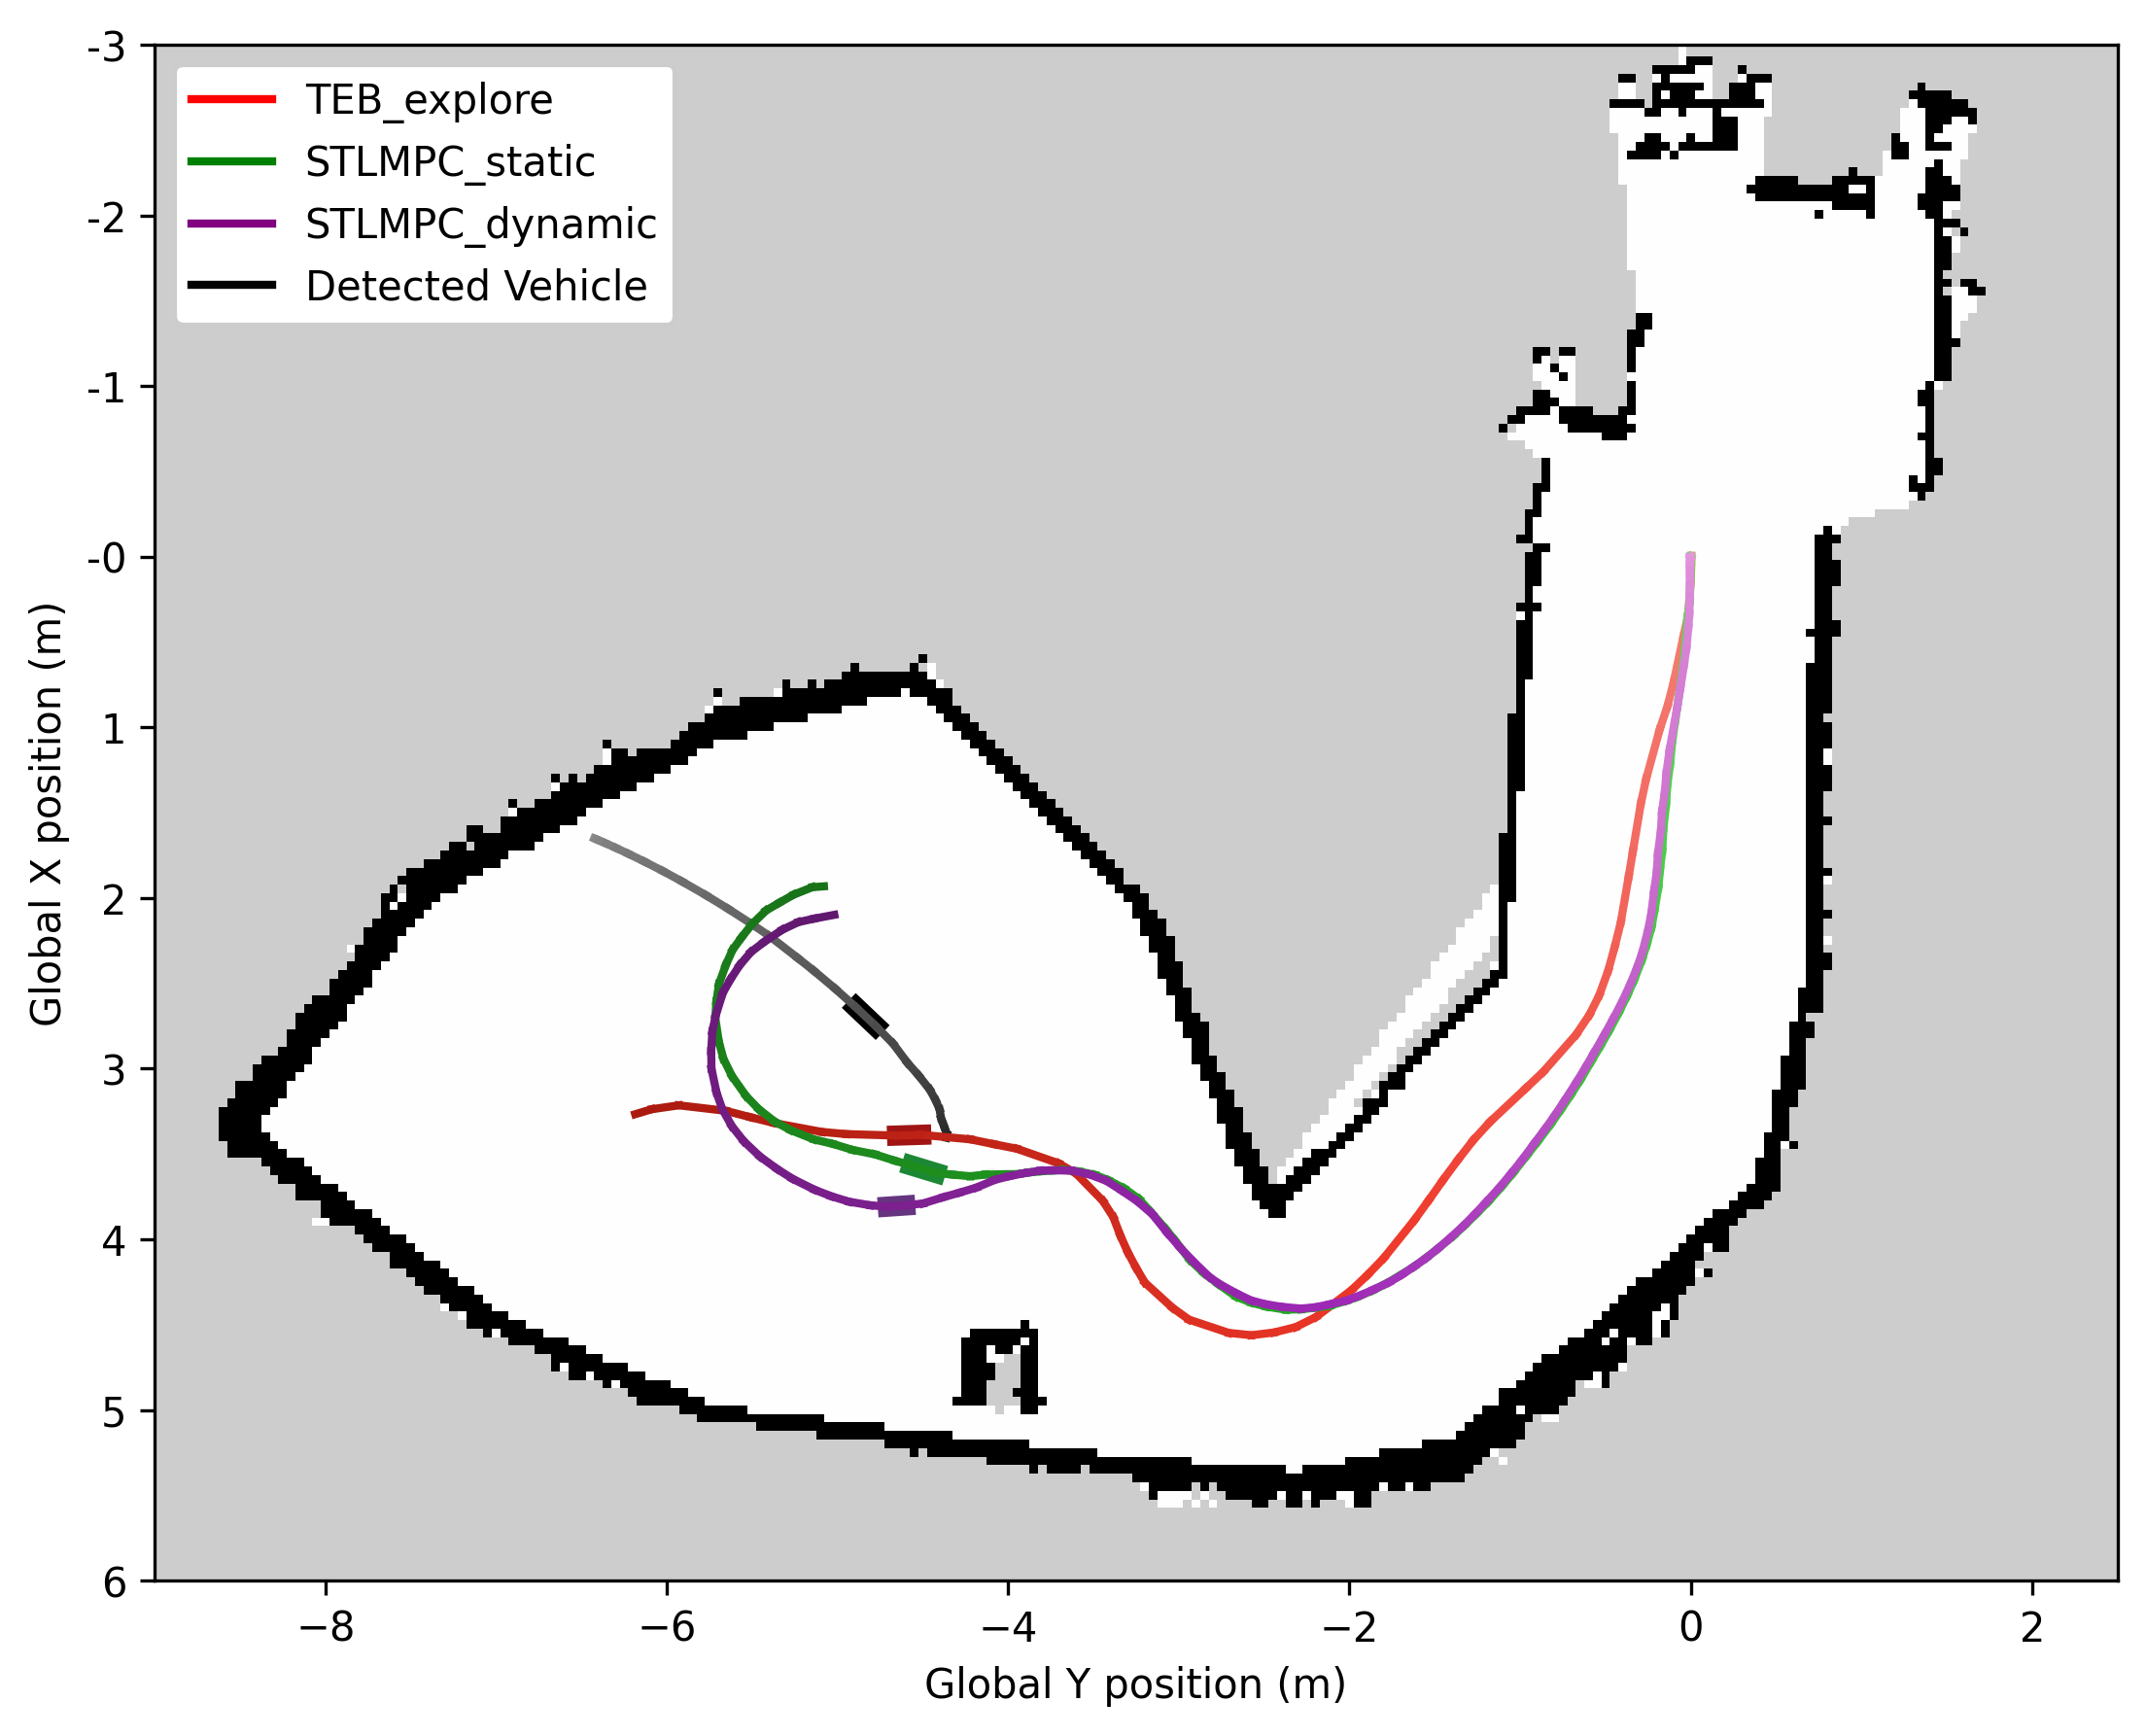
\includegraphics[width=0.75\columnwidth]{Figures/Exp4avoidROT.png}
    \caption[Compared local planner trajectories for dynamic obstacle avoidance in Experiment \#2]{Local planner trajectories for dynamic obstacle avoidance in Experiment \#2. Darker gradients denote time progression. One shared time sample before vehicle avoidance is indicated by a point on each path.}
	\label{Chap4expavoid}
\end{figure}

\begin{table}[ht]
  \caption{Performance of local planners including dynamic obstacle STLMPC in Experiment \#2}
  \label{tab:STLMPCexp4}
  \vspace{-8pt}
  \centering
  \begin{tabular}{l@{\hskip 3.4pt}c@{\hskip 4pt}c@{\hskip 5pt}c@{\hskip 4pt}c@{\hskip 4pt}c@{\hskip 4pt}c}
    \toprule\\[-0.85em]
    \scriptsize Local Planner & \makecell{\scriptsize$\min_{\tilde k} d_{\textup{min},\tilde k}$\\[0.25em](m)} & \makecell{\scriptsize$\bar{d}_\textup{min}$\\[0.3em](m)} & \makecell{\scriptsize$\overline{|\delta_{\textup{cmd},\tilde k}|}$\\[0.2em](rad)} & \makecell{\scriptsize$\mathrm{Var}(\delta_{\textup{cmd},\tilde k})$\\[0.2em]($\textup{rad}^2$)} & \makecell{\scriptsize$\bar{v}_{\textup{cmd},\tilde k}$\\[0.3em](m/s)} & \makecell{\scriptsize$\mathrm{Var}(v_{\textup{cmd},\tilde k})$\\[0.2em]($\textup{m}^2$/$\textup{s}^2$)}\\
    \midrule\\[-0.85em]
    \scriptsize TEB\_explore      & 0.487 & 0.846 & 0.181 & 0.050 & 1.249 & 0.142 \\
    \scriptsize STLMPC\_sta     & 0.531 & 0.908 & 0.195 & 0.048 & 1.211 & 0.069  \\
    \scriptsize STLMPC\_dyn   & 0.562 & 0.910 & 0.196 & 0.045 & 1.234 & 0.053  \\
    \bottomrule
  \end{tabular}
\end{table}

\begin{table}[!ht]
\caption{Planning computation times for local planners including dynamic obstacle STLMPC in Experiment \#2}
\label{tab:STLMPCcomp4}
\vspace{-8pt}
\centering
\begin{tabular}{
    l@{\hskip 2.4pt}c@{\hskip 4.0pt}c@{\hskip 4.0pt}c@{\hskip 5.5pt}c@{\hskip 3.2pt}c@{\hskip 3.2pt}c@{\hskip 3.2pt}c@{\hskip 3.2pt}c
}
\toprule\\[-1.2em]
\scriptsize Local Planner &
\makecell{\scriptsize$\bar{t}_\textup{frn}$\\(ms)} &
\makecell{\scriptsize$\bar{t}_\textup{glb}$\\(ms)} &
\makecell{\scriptsize$\bar{t}_\textup{loc}$\\(ms)} &
\makecell{\scriptsize\bm{$\bar{t}_\textbf{comp}$}\\\textbf{(ms)}} &
\makecell{\scriptsize$\max t_\textup{frn}$\\(ms)} &
\makecell{\scriptsize$\max t_\textup{glb}$\\(ms)} &
\makecell{\scriptsize$\max t_\textup{loc}$\\(ms)} &
\makecell{\scriptsize$\bm{\max t_\textbf{comp}}$\\\textbf{(ms)}} \\
\midrule\\[-1.2em] 
{\scriptsize TEB\_explore} & 1.7 & 0.9 & 3.7 & \textbf{6.3} & 2.5 & 3.4 & 13.6 & \textbf{19.6}  \\
{\scriptsize STLMPC\_sta} & \multicolumn{3}{c}{~~~} & \textbf{6.4} & \multicolumn{3}{c}{~~~} & \textbf{12.7}  \\
{\scriptsize STLMPC\_dyn} & \multicolumn{3}{c}{~~~} & \textbf{6.8} & \multicolumn{3}{c}{~~~} & \textbf{42.3}  \\
\bottomrule
\end{tabular}
\end{table}

\subsection{Racing on an Unknown Course}\label{sec:exp3}
In a third experiment (Fig. \ref{CourseLayouts3}), variable-velocity STLMPC is tested against other local planners in a racing context, where the fastest course time is desired. The track contains tight corners, meaning a large, constant velocity will lead to crashes. Thus, a varying velocity is required, which reduces for turns and increases for straightaways. Existing STLMPC parameters are maintained while the velocity-related parameters are now activated as listed in Table \ref{tab:params}, with $d_\textup{safe}$ reduced to 1.25 m to accommodate the tighter track. This track poses challenges to a number of the tested local planners, where only a select few complete the course.

DWA- and MPC-based exploration proceed very slowly and repeatedly run into obstacles in this setup; therefore, they are not included in the results. Furthermore, the PD approach fails to successfully navigate the first turn, even at low speeds, crashing early on in the course. The TEB-based planner fails at high speeds, but when the maximum speed is reduced to 1 m/s, the vehicle is able to complete the course, although it encounters collisions at two specific track sections. Constant-velocity STLMPC at 3 m/s fails but succeeds at 1.5 m/s while variable-velocity STLMPC uses $v_\textup{min}\!=\!0$ m/s and $v_\textup{max}\!=\!3$ m/s.

The trajectories of the planners that complete the course are shown in Fig. \ref{Chap5exptraj}. Variable-velocity STLMPC takes several corners tighter than constant-velocity STLMPC and sacrifices safety in some spots to achieve a faster track time. Operating at faster speeds means less reaction time and poorer maneuverability; however, adequate safety is maintained through the added velocity constraints, and a visibly safe path is produced. The TEB-based planner completes the course but collides near the middle section and towards the end due to the sharp turns.

\begin{figure}[ht]
    \centering
    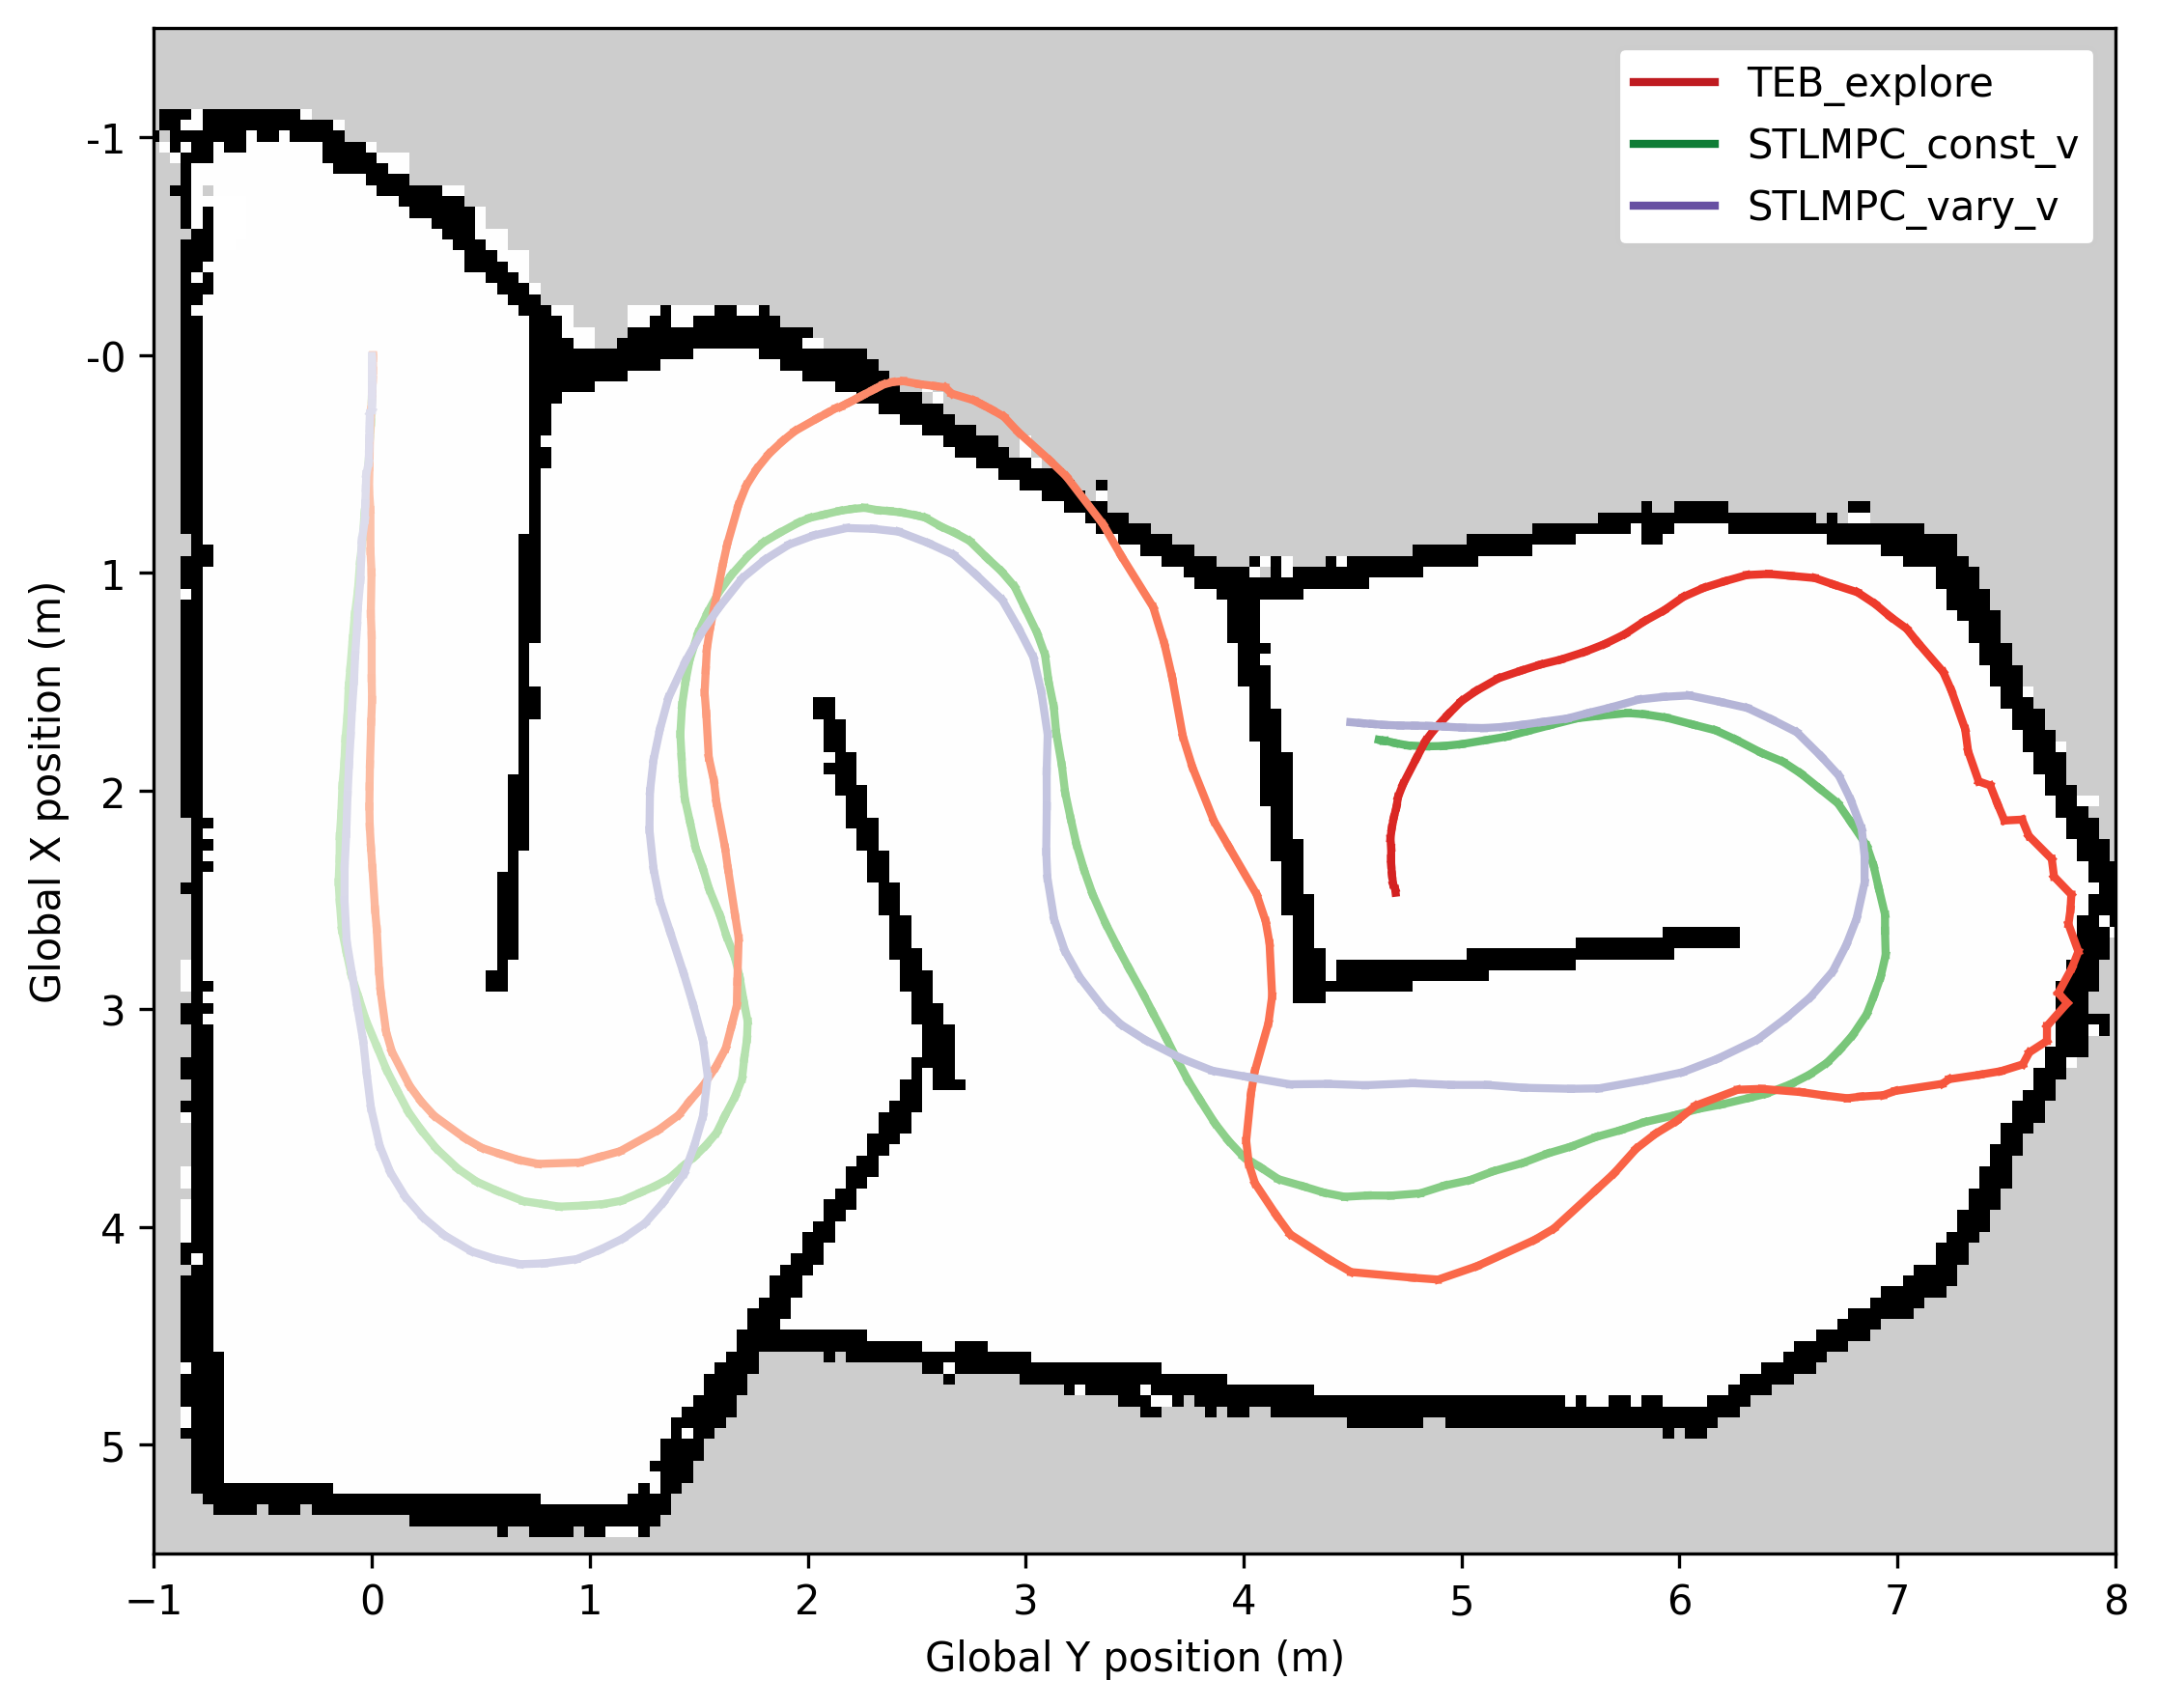
\includegraphics[width=0.75\columnwidth]{Figures/Exp5TrajsROT.png}
    \caption[Variable-velocity STLMPC and other local planner trajectories in Experiment \#3]{Local planner trajectories including for variable-velocity STLMPC in Experiment \#3. Darker color gradients for each path show time progression, where variable-velocity STLMPC is lightest as it completes the course fastest.}
	\label{Chap5exptraj}
\end{figure}

The planners are further evaluated in Table \ref{tab:STLMPCexp5}, which presents proximity, control input and total track time $t_\textup{tot}$ metrics. The minimum obstacle proximity for the TEB planner is not applicable, as collision occurs, while variable-velocity STLMPC attains poorer proximity metrics compared to constant-velocity STLMPC due to more aggressive motion at higher speeds. However, velocity-varying STLMPC achieves the lowest steering angle average magnitude and variance due to its direct, fast motion on straight track sections.

\begin{table}[ht]
  \caption{Performance of local planners including variable-velocity STLMPC in Experiment \#3}
  \label{tab:STLMPCexp5}
  \vspace{-8pt}
  \centering
  \begin{tabular}{l@{\hskip 0.4pt}c@{\hskip 2pt}c@{\hskip 2pt}c@{\hskip 2pt}c@{\hskip 2pt}c@{\hskip 2pt}c@{\hskip 1pt}c}
    \toprule\\[-0.85em]
    \scriptsize Local Planner & \makecell{\scriptsize$\min_{\tilde k} d_{\textup{min},\tilde k}$\\[0.25em](m)} & \makecell{\scriptsize$\bar{d}_\textup{min}$\\[0.3em](m)} & \makecell{\scriptsize$\overline{|\delta_{\textup{cmd},\tilde k}|}$\\[0.2em](rad)} & \makecell{\scriptsize$\mathrm{Var}(\delta_{\textup{cmd},\tilde k})$\\[0.2em]($\textup{rad}^2$)} & \makecell{\scriptsize$\bar{v}_{\textup{cmd},\tilde k}$\\[0.3em](m/s)} & \makecell{\scriptsize$\mathrm{Var}(v_{\textup{cmd},\tilde k})$\\[0.2em]($\textup{m}^2$/$\textup{s}^2$)} & \makecell{\scriptsize$t_\textup{tot}$\\[0.35em](s)}\\
    \midrule\\[-0.85em]
    \scriptsize TEB\_explore      & N/A & 0.532 & 0.261 & 0.086 & 0.863 & 0.092 & 25.4 \\
    \scriptsize STLMPC\_con     & 0.528 & 0.747 & 0.224 & 0.068 & 1.176 & 0.082 & 15.8  \\
    \scriptsize STLMPC\_var   & 0.403 & 0.720 & 0.196 & 0.057 & 1.456 & 0.331 & 12.8  \\
    \bottomrule
  \end{tabular}
\end{table}

The variable-velocity method achieves the fastest average velocity and track time. Dynamic speeds over 2 m/s are achieved on straight track sections while the turning-angle and obstacle-proximity upper limits on velocity are adhered to. Planning times are provided for each method in Table \ref{tab:STLMPCcomp5}, where velocity-varying STLMPC has significantly longer times compared to constant-velocity STLMPC. The additional velocity variables and constraints add dimensionality to the optimization, increasing the complexity. Still, solutions are found reliably within the control period, while in the worst case, the solver terminates gracefully after timing out at 50 ms. TEB struggles with the course's sharp turns, where the worst-case planning time occurs, exceeding the control period.

\begin{table}[ht]
\caption{Planning computation times for local planners including variable-velocity STLMPC in Experiment \#3}
\label{tab:STLMPCcomp5}
\vspace{-8pt}
\centering
\begin{tabular}{
    l@{\hskip 2.4pt}c@{\hskip 4.0pt}c@{\hskip 4.0pt}c@{\hskip 5.5pt}c@{\hskip 3.2pt}c@{\hskip 3.2pt}c@{\hskip 3.2pt}c@{\hskip 3.2pt}c
}
\toprule\\[-1.2em]
\scriptsize Local Planner &
\makecell{\scriptsize$\bar{t}_\textup{frn}$\\(ms)} &
\makecell{\scriptsize$\bar{t}_\textup{glb}$\\(ms)} &
\makecell{\scriptsize$\bar{t}_\textup{loc}$\\(ms)} &
\makecell{\scriptsize\bm{$\bar{t}_\textbf{comp}$}\\\textbf{(ms)}} &
\makecell{\scriptsize$\max t_\textup{frn}$\\(ms)} &
\makecell{\scriptsize$\max t_\textup{glb}$\\(ms)} &
\makecell{\scriptsize$\max t_\textup{loc}$\\(ms)} &
\makecell{\scriptsize$\bm{\max t_\textbf{comp}}$\\\textbf{(ms)}} \\
\midrule\\[-1.2em] 
{\scriptsize TEB\_explore} & 4.5 & 1.0 & 8.6 & \textbf{14.1} & 14.6 & 2.5 & 102.4 & \textbf{119.6}  \\
{\scriptsize STLMPC\_con} & \multicolumn{3}{c}{~~~} & \phantom{0}\textbf{6.7} & \multicolumn{3}{c}{~~~} & \phantom{0}\textbf{18.9}  \\
{\scriptsize STLMPC\_var} & \multicolumn{3}{c}{~~~} & \textbf{32.2} & \multicolumn{3}{c}{~~~} & \phantom{0}\textbf{61.4}  \\
\bottomrule
\end{tabular}
\end{table}


\subsection{Discussion and Limitations}\label{sec:limitations}
Several limitations are disclosed. First, the receding-horizon scheme carries no formal closed-loop stability or recursive-feasibility guarantee; in place of a proof, practical stability is supported empirically by the feasible warm start, the feasibility-preserving timeout, and the convergence statistics reported above. Second, the kinematic bicycle model is valid only for low tire slip and lateral acceleration \cite{Polack2017}; the steering-based velocity limit \eqref{5.3.5} acts to keep operation inside this envelope, but model mismatch may grow under the most aggressive maneuvers. Third, adversary prediction assumes constant velocity and curvature, so accuracy degrades under sudden braking or sharp turns---the extent of this degradation is characterized by the R1/R2 robustness rows above. Finally, detection robustness under low-light or heavy-occlusion conditions is inherited from the perception module and is outside the scope of the planner evaluated here.

\section{Conclusion}\label{sec7} %Also include future work briefly
In this article, the formulation of a novel, open-source, standalone local path planner was outlined for safe navigation in unknown surroundings. Sequential local reference tracking lines are generated at each control step through quadratic optimizations before a non-convex MPC optimization incorporates nonholonomic system constraints within trajectory prediction. Dynamic obstacles are considered through a complete detection, tracking and avoidance framework, while racing applications are accommodated through an adaptation which promotes higher speeds when safe. In unknown static, dynamic and racing environments, both in simulated and real-world tests, local planning using this novel algorithm attains improved obstacle clearance and lower control effort relative to exploration-based schemes configured for goal-free navigation, with component-wise ablations isolating the contribution of the sequential tracking lines, the dynamic-obstacle branch and the racing velocity constraints.

Possible future directions for this work include accommodating different kinematic models for varying robots and using reinforcement learning for adaptive parameters based on past navigation experience. Other potential extensions involve integration in hierarchical planning to map and explore unknown regions, as well as the incorporation of vehicle reversal.

%Appendix?

%References
\bibliographystyle{IEEEtran}
\bibliography{references}

%Biographies?
% \begin{IEEEbiography}{Author 1 Placeholder Bibliography}
% Placeholder bibliography text here.
% \end{IEEEbiography}

% \begin{IEEEbiography}{Author 2 Placeholder Bibliography}
% Placeholder bibliography text here.
% \end{IEEEbiography}


\end{document}


